% concatenated from arxiv_version_2025.tex, math_commands.tex
\documentclass{article}
\usepackage[numbers,compress]{natbib}

% if you need to pass options to natbib, use, \emph{e.g.}:
%     \PassOptionsToPackage{numbers, compress}{natbib}
% before loading neurips_2025


% ready for submission
%\usepackage{neurips_2025}


% to compile a preprint version, \emph{e.g.}, for submission to arXiv, add add the
% [preprint] option:
\usepackage[preprint]{neurips_2025}


% to compile a camera-ready version, add the [final] option, \emph{e.g.}:
%     \usepackage[final]{neurips_2025}


% to avoid loading the natbib package, add option nonatbib:
%    \usepackage[nonatbib]{neurips_2025}


\usepackage[utf8]{inputenc} % allow utf-8 input
\usepackage[T1]{fontenc}    % use 8-bit T1 fonts
\usepackage{hyperref}       % hyperlinks
\usepackage{url}            % simple URL typesetting
\usepackage{booktabs}       % professional-quality tables
\usepackage{amsfonts}       % blackboard math symbols
\usepackage{nicefrac}       % compact symbols for 1/2, \emph{etc.}
\usepackage{microtype}      % microtypography
\usepackage[table]{xcolor}         % colors with table option
\usepackage{graphicx}
\usepackage{wrapfig}
\usepackage{subcaption}
\usepackage{caption}
\usepackage{tcolorbox}

\usepackage[ruled,linesnumbered]{algorithm2e}
\usepackage{appendix}
\usepackage{amsthm,amssymb,amsmath,amsfonts}
\usepackage{comment}
\usepackage{enumitem}
\usepackage{tikz}
\usepackage{tablefootnote}
\usetikzlibrary{arrows.meta}
\usetikzlibrary{decorations.pathreplacing}
\usetikzlibrary{positioning}
\usetikzlibrary{calc}
\usetikzlibrary{backgrounds}

\usepackage{cellspace}

\usepackage{tikz-cd}
\usepackage{multirow} 
\usepackage{enumitem}
\usepackage{makecell}

\numberwithin{equation}{section}

\newtheorem{theorem}{Theorem}[section]
\newtheorem{lemma}[theorem]{Lemma}
\newtheorem{assumption}{Assumption}[section]
\newtheorem{corollary}[theorem]{Corollary}
\newtheorem{definition}[theorem]{Definition}
\newtheorem{proposition}[theorem]{Proposition}
\newtheorem{remark}[theorem]{Remark}

%%%%% NEW MATH DEFINITIONS %%%%%

\usepackage{amsmath,amsfonts,bm}
% Mark sections of captions for referring to divisions of figures
\newcommand{\figleft}{{\em (Left)}}
\newcommand{\figcenter}{{\em (Center)}}
\newcommand{\figright}{{\em (Right)}}
\newcommand{\figtop}{{\em (Top)}}
\newcommand{\figbottom}{{\em (Bottom)}}
\newcommand{\captiona}{{\em (a)}}
\newcommand{\captionb}{{\em (b)}}
\newcommand{\captionc}{{\em (c)}}
\newcommand{\captiond}{{\em (d)}}
\DeclareMathOperator{\Tr}{Tr} 

% Highlight a newly defined term
\newcommand{\newterm}[1]{{\bf #1}}
\newcommand{\unif}{\mathrm{Unif}}

% Figure reference, lower-case.
\def\figref#1{figure~\ref{#1}}
% Figure reference, capital. For start of sentence
\def\Figref#1{Figure~\ref{#1}}
\def\twofigref#1#2{figures \ref{#1} and \ref{#2}}
\def\quadfigref#1#2#3#4{figures \ref{#1}, \ref{#2}, \ref{#3} and \ref{#4}}
% Section reference, lower-case.
\def\secref#1{Section~\ref{#1}}
% Reference to two sections.
\def\twosecrefs#1#2{Sections \ref{#1} and \ref{#2}}
% Reference to three sections.
\def\secrefs#1#2#3{Sections \ref{#1}, \ref{#2} and \ref{#3}}
% Reference to an equation, lower-case.
\def\eqref#1{(\ref{#1})}
% Reference to an equation, upper case
\def\Eqref#1{Equation~\ref{#1}}
% A raw reference to an equation---avoid using if possible
\def\plaineqref#1{\ref{#1}}
% Reference to a chapter, lower-case.
\def\chapref#1{Chapter~\ref{#1}}
% Reference to a range of chapters
\def\rangechapref#1#2{Chapters\ref{#1}--\ref{#2}}
% Reference to an algorithm, lower-case.
\def\algref#1{Algorithm~\ref{#1}}
\def\twoalgref#1#2{Algorithms \ref{#1} and \ref{#2}}
% Reference to a part, lower case
\def\partref#1{Part~\ref{#1}}
\def\twopartref#1#2{Parts \ref{#1} and \ref{#2}}

\def\ceil#1{\lceil #1 \rceil}
\def\floor#1{\lfloor #1 \rfloor}
\def\angle#1{\langle #1 \rangle}

\newcommand{\dif}{{\mathrm{d}}}
\def\eps{{\epsilon}}



% Random variables
\def\reta{{\textnormal{$\eta$}}}
\def\ra{{\textnormal{a}}}
\def\rb{{\textnormal{b}}}
\def\rc{{\textnormal{c}}}
\def\rd{{\textnormal{d}}}
\def\re{{\textnormal{e}}}
\def\rf{{\textnormal{f}}}
\def\rg{{\textnormal{g}}}
\def\rh{{\textnormal{h}}}
\def\ri{{\textnormal{i}}}
\def\rj{{\textnormal{j}}}
\def\rk{{\textnormal{k}}}
\def\rl{{\textnormal{l}}}
% rm is already a command, just don't name any random variables m
\def\rn{{\textnormal{n}}}
\def\ro{{\textnormal{o}}}
\def\rp{{\textnormal{p}}}
\def\rq{{\textnormal{q}}}
\def\rr{{\textnormal{r}}}
\def\rs{{\textnormal{s}}}
\def\rt{{\textnormal{t}}}
\def\ru{{\textnormal{u}}}
\def\rv{{\textnormal{v}}}
\def\rw{{\textnormal{w}}}
\def\rx{{\textnormal{x}}}
\def\ry{{\textnormal{y}}}
\def\rz{{\textnormal{z}}}

% Random vectors
\def\rvepsilon{{\mathbf{\epsilon}}}
\def\rvtheta{{\mathbf{\theta}}}
\def\rva{{\mathbf{a}}}
\def\rvb{{\mathbf{b}}}
\def\rvc{{\mathbf{c}}}
\def\rvd{{\mathbf{d}}}
\def\rve{{\mathbf{e}}}
\def\rvf{{\mathbf{f}}}
\def\rvg{{\mathbf{g}}}
\def\rvh{{\mathbf{h}}}
\def\rvu{{\mathbf{i}}}
\def\rvj{{\mathbf{j}}}
\def\rvk{{\mathbf{k}}}
\def\rvl{{\mathbf{l}}}
\def\rvm{{\mathbf{m}}}
\def\rvn{{\mathbf{n}}}
\def\rvo{{\mathbf{o}}}
\def\rvp{{\mathbf{p}}}
\def\rvq{{\mathbf{q}}}
\def\rvr{{\mathbf{r}}}
\def\rvs{{\mathbf{s}}}
\def\rvt{{\mathbf{t}}}
\def\rvu{{\mathbf{u}}}
\def\rvv{{\mathbf{v}}}
\def\rvw{{\mathbf{w}}}
\def\rvx{{\mathbf{x}}}
\def\rvy{{\mathbf{y}}}
\def\rvz{{\mathbf{z}}}

% Elements of random vectors
\def\erva{{\textnormal{a}}}
\def\ervb{{\textnormal{b}}}
\def\ervc{{\textnormal{c}}}
\def\ervd{{\textnormal{d}}}
\def\erve{{\textnormal{e}}}
\def\ervf{{\textnormal{f}}}
\def\ervg{{\textnormal{g}}}
\def\ervh{{\textnormal{h}}}
\def\ervi{{\textnormal{i}}}
\def\ervj{{\textnormal{j}}}
\def\ervk{{\textnormal{k}}}
\def\ervl{{\textnormal{l}}}
\def\ervm{{\textnormal{m}}}
\def\ervn{{\textnormal{n}}}
\def\ervo{{\textnormal{o}}}
\def\ervp{{\textnormal{p}}}
\def\ervq{{\textnormal{q}}}
\def\ervr{{\textnormal{r}}}
\def\ervs{{\textnormal{s}}}
\def\ervt{{\textnormal{t}}}
\def\ervu{{\textnormal{u}}}
\def\ervv{{\textnormal{v}}}
\def\ervw{{\textnormal{w}}}
\def\ervx{{\textnormal{x}}}
\def\ervy{{\textnormal{y}}}
\def\ervz{{\textnormal{z}}}

% Random matrices
\def\rmA{{\mathbf{A}}}
\def\rmB{{\mathbf{B}}}
\def\rmC{{\mathbf{C}}}
\def\rmD{{\mathbf{D}}}
\def\rmE{{\mathbf{E}}}
\def\rmF{{\mathbf{F}}}
\def\rmG{{\mathbf{G}}}
\def\rmH{{\mathbf{H}}}
\def\rmI{{\mathbf{I}}}
\def\rmJ{{\mathbf{J}}}
\def\rmK{{\mathbf{K}}}
\def\rmL{{\mathbf{L}}}
\def\rmM{{\mathbf{M}}}
\def\rmN{{\mathbf{N}}}
\def\rmO{{\mathbf{O}}}
\def\rmP{{\mathbf{P}}}
\def\rmQ{{\mathbf{Q}}}
\def\rmR{{\mathbf{R}}}
\def\rmS{{\mathbf{S}}}
\def\rmT{{\mathbf{T}}}
\def\rmU{{\mathbf{U}}}
\def\rmV{{\mathbf{V}}}
\def\rmW{{\mathbf{W}}}
\def\rmX{{\mathbf{X}}}
\def\rmY{{\mathbf{Y}}}
\def\rmZ{{\mathbf{Z}}}

% Elements of random matrices
\def\ermA{{\textnormal{A}}}
\def\ermB{{\textnormal{B}}}
\def\ermC{{\textnormal{C}}}
\def\ermD{{\textnormal{D}}}
\def\ermE{{\textnormal{E}}}
\def\ermF{{\textnormal{F}}}
\def\ermG{{\textnormal{G}}}
\def\ermH{{\textnormal{H}}}
\def\ermI{{\textnormal{I}}}
\def\ermJ{{\textnormal{J}}}
\def\ermK{{\textnormal{K}}}
\def\ermL{{\textnormal{L}}}
\def\ermM{{\textnormal{M}}}
\def\ermN{{\textnormal{N}}}
\def\ermO{{\textnormal{O}}}
\def\ermP{{\textnormal{P}}}
\def\ermQ{{\textnormal{Q}}}
\def\ermR{{\textnormal{R}}}
\def\ermS{{\textnormal{S}}}
\def\ermT{{\textnormal{T}}}
\def\ermU{{\textnormal{U}}}
\def\ermV{{\textnormal{V}}}
\def\ermW{{\textnormal{W}}}
\def\ermX{{\textnormal{X}}}
\def\ermY{{\textnormal{Y}}}
\def\ermZ{{\textnormal{Z}}}

% Vectors
\def\vzero{{\bm{0}}}
\def\vone{{\bm{1}}}

\def\va{{\bm{a}}}
\def\vb{{\bm{b}}}
\def\vc{{\bm{c}}}
\def\vd{{\bm{d}}}
\def\ve{{\bm{e}}}
\def\vf{{\bm{f}}}
\def\vg{{\bm{g}}}
\def\vh{{\bm{h}}}
\def\vi{{\bm{i}}}
\def\vj{{\bm{j}}}
\def\vk{{\bm{k}}}
\def\vl{{\bm{l}}}
\def\vm{{\bm{m}}}
\def\vn{{\bm{n}}}
\def\vo{{\bm{o}}}
\def\vp{{\bm{p}}}
\def\vq{{\bm{q}}}
\def\vr{{\bm{r}}}
\def\vs{{\bm{s}}}
\def\vt{{\bm{t}}}
\def\vu{{\bm{u}}}
\def\vv{{\bm{v}}}
\def\vw{{\bm{w}}}
\def\vx{{\bm{x}}}
\def\vy{{\bm{y}}}
\def\vz{{\bm{z}}}

\def\valpha{{\bm{\alpha}}}
\def\vbeta{{\bm{\beta}}}
\def\vgamma{{\bm{\gamma}}}
\def\vdelta{{\bm{\delta}}}
\def\vepsilon{{\bm{\epsilon}}}
\def\vzeta{{\bm{\zeta}}}
\def\veta{{\bm{\eta}}}
\def\vtheta{{\bm{\theta}}}
\def\viota{{\bm{\iota}}}
\def\vkappa{{\bm{\kappa}}}
\def\vlambda{{\bm{\lambda}}}
\def\vmu{{\bm{\mu}}}
\def\vnu{{\bm{\nu}}}
\def\vxi{{\bm{\xi}}}
\def\vpi{{\bm{\pi}}}
\def\vrho{{\bm{\rho}}}
\def\vsigma{{\bm{\sigma}}}
\def\vtau{{\bm{\tau}}}
\def\vupsilon{{\bm{\upsilon}}}
\def\vphi{{\bm{\phi}}}
\def\vchi{{\bm{\chi}}}
\def\vpsi{{\bm{\psi}}}
\def\vomega{{\bm{\omega}}}




% Elements of vectors
\def\evalpha{{\alpha}}
\def\evbeta{{\beta}}
\def\evepsilon{{\epsilon}}
\def\evlambda{{\lambda}}
\def\evomega{{\omega}}
\def\evmu{{\mu}}
\def\evpsi{{\psi}}
\def\evsigma{{\sigma}}
\def\evtheta{{\theta}}
\def\eva{{a}}
\def\evb{{b}}
\def\evc{{c}}
\def\evd{{d}}
\def\eve{{e}}
\def\evf{{f}}
\def\evg{{g}}
\def\evh{{h}}
\def\evi{{i}}
\def\evj{{j}}
\def\evk{{k}}
\def\evl{{l}}
\def\evm{{m}}
\def\evn{{n}}
\def\evo{{o}}
\def\evp{{p}}
\def\evq{{q}}
\def\evr{{r}}
\def\evs{{s}}
\def\evt{{t}}
\def\evu{{u}}
\def\evv{{v}}
\def\evw{{w}}
\def\evx{{x}}
\def\evy{{y}}
\def\evz{{z}}

% Matrix
\def\mA{{\bm{A}}}
\def\mB{{\bm{B}}}
\def\mC{{\bm{C}}}
\def\mD{{\bm{D}}}
\def\mE{{\bm{E}}}
\def\mF{{\bm{F}}}
\def\mG{{\bm{G}}}
\def\mH{{\bm{H}}}
\def\mI{{\bm{I}}}
\def\mJ{{\bm{J}}}
\def\mK{{\bm{K}}}
\def\mL{{\bm{L}}}
\def\mM{{\bm{M}}}
\def\mN{{\bm{N}}}
\def\mO{{\bm{O}}}
\def\mP{{\bm{P}}}
\def\mQ{{\bm{Q}}}
\def\mR{{\bm{R}}}
\def\mS{{\bm{S}}}
\def\mT{{\bm{T}}}
\def\mU{{\bm{U}}}
\def\mV{{\bm{V}}}
\def\mW{{\bm{W}}}
\def\mX{{\bm{X}}}
\def\mY{{\bm{Y}}}
\def\mZ{{\bm{Z}}}

\def\mAlpha{{\bm{\Alpha}}}
\def\mBeta{{\bm{\Beta}}}
\def\mGamma{{\bm{\Gamma}}}
\def\mDelta{{\bm{\Delta}}}
\def\mEpsilon{{\bm{\Epsilon}}}
\def\mZeta{{\bm{\Zeta}}}
\def\mEta{{\bm{\Eta}}}
\def\mTheta{{\bm{\Theta}}}
\def\mIota{{\bm{\Iota}}}
\def\mKappa{{\bm{\Kappa}}}
\def\mLambda{{\bm{\Lambda}}}
\def\mMu{{\bm{\Mu}}}
\def\mNu{{\bm{\Nu}}}
\def\mXi{{\bm{\Xi}}}
\def\mPi{{\bm{\Pi}}}
\def\mRho{{\bm{\Rho}}}
\def\mSigma{{\bm{\Sigma}}}
\def\mTau{{\bm{\Tau}}}
\def\mUpsilon{{\bm{\Upsilon}}}
\def\mPhi{{\bm{\Phi}}}
\def\mChi{{\bm{\Chi}}}
\def\mPsi{{\bm{\Psi}}}
\def\mOmega{{\bm{\Omega}}}


% Tensor
\DeclareMathAlphabet{\mathsfit}{\encodingdefault}{\sfdefault}{m}{sl}
\SetMathAlphabet{\mathsfit}{bold}{\encodingdefault}{\sfdefault}{bx}{n}
\newcommand{\tens}[1]{\bm{\mathsfit{#1}}}
\def\tA{{\tens{A}}}
\def\tB{{\tens{B}}}
\def\tC{{\tens{C}}}
\def\tD{{\tens{D}}}
\def\tE{{\tens{E}}}
\def\tF{{\tens{F}}}
\def\tG{{\tens{G}}}
\def\tH{{\tens{H}}}
\def\tI{{\tens{I}}}
\def\tJ{{\tens{J}}}
\def\tK{{\tens{K}}}
\def\tL{{\tens{L}}}
\def\tM{{\tens{M}}}
\def\tN{{\tens{N}}}
\def\tO{{\tens{O}}}
\def\tP{{\tens{P}}}
\def\tQ{{\tens{Q}}}
\def\tR{{\tens{R}}}
\def\tS{{\tens{S}}}
\def\tT{{\tens{T}}}
\def\tU{{\tens{U}}}
\def\tV{{\tens{V}}}
\def\tW{{\tens{W}}}
\def\tX{{\tens{X}}}
\def\tY{{\tens{Y}}}
\def\tZ{{\tens{Z}}}


% Graph
\def\gA{{\mathcal{A}}}
\def\gB{{\mathcal{B}}}
\def\gC{{\mathcal{C}}}
\def\gD{{\mathcal{D}}}
\def\gE{{\mathcal{E}}}
\def\gF{{\mathcal{F}}}
\def\gG{{\mathcal{G}}}
\def\gH{{\mathcal{H}}}
\def\gI{{\mathcal{I}}}
\def\gJ{{\mathcal{J}}}
\def\gK{{\mathcal{K}}}
\def\gL{{\mathcal{L}}}
\def\gM{{\mathcal{M}}}
\def\gN{{\mathcal{N}}}
\def\gO{{\mathcal{O}}}
\def\gP{{\mathcal{P}}}
\def\gQ{{\mathcal{Q}}}
\def\gR{{\mathcal{R}}}
\def\gS{{\mathcal{S}}}
\def\gT{{\mathcal{T}}}
\def\gU{{\mathcal{U}}}
\def\gV{{\mathcal{V}}}
\def\gW{{\mathcal{W}}}
\def\gX{{\mathcal{X}}}
\def\gY{{\mathcal{Y}}}
\def\gZ{{\mathcal{Z}}}

% Sets
\def\sA{{\mathbb{A}}}
\def\sB{{\mathbb{B}}}
\def\sC{{\mathbb{C}}}
\def\sD{{\mathbb{D}}}
% Don't use a set called E, because this would be the same as our symbol
% for expectation.
\def\sF{{\mathbb{F}}}
\def\sG{{\mathbb{G}}}
\def\sH{{\mathbb{H}}}
\def\sI{{\mathbb{I}}}
\def\sJ{{\mathbb{J}}}
\def\sK{{\mathbb{K}}}
\def\sL{{\mathbb{L}}}
\def\sM{{\mathbb{M}}}
\def\sN{{\mathbb{N}}}
\def\sO{{\mathbb{O}}}
\def\sP{{\mathbb{P}}}
\def\sQ{{\mathbb{Q}}}
\def\sR{{\mathbb{R}}}
\def\sS{{\mathbb{S}}}
\def\sT{{\mathbb{T}}}
\def\sU{{\mathbb{U}}}
\def\sV{{\mathbb{V}}}
\def\sW{{\mathbb{W}}}
\def\sX{{\mathbb{X}}}
\def\sY{{\mathbb{Y}}}
\def\sZ{{\mathbb{Z}}}

% Entries of a matrix
\def\emLambda{{\Lambda}}
\def\emA{{A}}
\def\emB{{B}}
\def\emC{{C}}
\def\emD{{D}}
\def\emE{{E}}
\def\emF{{F}}
\def\emG{{G}}
\def\emH{{H}}
\def\emI{{I}}
\def\emJ{{J}}
\def\emK{{K}}
\def\emL{{L}}
\def\emM{{M}}
\def\emN{{N}}
\def\emO{{O}}
\def\emP{{P}}
\def\emQ{{Q}}
\def\emR{{R}}
\def\emS{{S}}
\def\emT{{T}}
\def\emU{{U}}
\def\emV{{V}}
\def\emW{{W}}
\def\emX{{X}}
\def\emY{{Y}}
\def\emZ{{Z}}
\def\emSigma{{\Sigma}}

% entries of a tensor
% Same font as tensor, without \bm wrapper
\newcommand{\etens}[1]{\mathsfit{#1}}
\def\etLambda{{\etens{\Lambda}}}
\def\etA{{\etens{A}}}
\def\etB{{\etens{B}}}
\def\etC{{\etens{C}}}
\def\etD{{\etens{D}}}
\def\etE{{\etens{E}}}
\def\etF{{\etens{F}}}
\def\etG{{\etens{G}}}
\def\etH{{\etens{H}}}
\def\etI{{\etens{I}}}
\def\etJ{{\etens{J}}}
\def\etK{{\etens{K}}}
\def\etL{{\etens{L}}}
\def\etM{{\etens{M}}}
\def\etN{{\etens{N}}}
\def\etO{{\etens{O}}}
\def\etP{{\etens{P}}}
\def\etQ{{\etens{Q}}}
\def\etR{{\etens{R}}}
\def\etS{{\etens{S}}}
\def\etT{{\etens{T}}}
\def\etU{{\etens{U}}}
\def\etV{{\etens{V}}}
\def\etW{{\etens{W}}}
\def\etX{{\etens{X}}}
\def\etY{{\etens{Y}}}
\def\etZ{{\etens{Z}}}

% \def\eta{{\etens{a}}}
\def\etb{{\etens{b}}}
\def\etc{{\etens{c}}}
\def\etd{{\etens{d}}}
\def\ete{{\etens{e}}}
\def\etf{{\etens{f}}}
\def\etg{{\etens{g}}}
% \def\eth{{\etens{h}}}
\def\eti{{\etens{i}}}
\def\etj{{\etens{j}}}
\def\etk{{\etens{k}}}
\def\etl{{\etens{l}}}
\def\etm{{\etens{m}}}
\def\etn{{\etens{n}}}
\def\eto{{\etens{o}}}
\def\etp{{\etens{p}}}
\def\etq{{\etens{q}}}
\def\etr{{\etens{r}}}
\def\ets{{\etens{s}}}
\def\ett{{\etens{t}}}
\def\etu{{\etens{u}}}
\def\etv{{\etens{v}}}
\def\etw{{\etens{w}}}
\def\etx{{\etens{x}}}
\def\ety{{\etens{y}}}
\def\etz{{\etens{z}}}














% The true underlying data generating distribution
\newcommand{\pdata}{p_{\rm{data}}}
% The empirical distribution defined by the training set
\newcommand{\ptrain}{\hat{p}_{\rm{data}}}
\newcommand{\Ptrain}{\hat{P}_{\rm{data}}}
% The model distribution
\newcommand{\pmodel}{p_{\rm{model}}}
\newcommand{\Pmodel}{P_{\rm{model}}}
\newcommand{\ptildemodel}{\tilde{p}_{\rm{model}}}
% Stochastic autoencoder distributions
\newcommand{\pencode}{p_{\rm{encoder}}}
\newcommand{\pdecode}{p_{\rm{decoder}}}
\newcommand{\precons}{p_{\rm{reconstruct}}}

\newcommand{\laplace}{\mathrm{Laplace}} % Laplace distribution

\newcommand{\E}{\mathbb{E}}
\renewcommand{\P}{\mathbb{P}}
\newcommand{\Ls}{\mathcal{L}}
\newcommand{\R}{\mathbb{R}}
\newcommand{\emp}{\tilde{p}}
\newcommand{\lr}{\alpha}
\newcommand{\reg}{\lambda}
\newcommand{\rect}{\mathrm{rectifier}}
\newcommand{\softmax}{\mathrm{softmax}}
\newcommand{\sigmoid}{\sigma}
\newcommand{\softplus}{\zeta}
\newcommand{\KL}{D_{\mathrm{KL}}}
\newcommand{\FI}{D_{\mathrm{FI}}}
\newcommand{\var}{\mathrm{var}}
\newcommand{\standarderror}{\mathrm{SE}}
\newcommand{\cov}{\mathrm{cov}}
\newcommand{\TV}{\mathrm{TV}}

% \newcommand{\ker}{\mathrm{Ker}}
\newcommand{\im}{\mathrm{Im}}
% Wolfram Mathworld says $L^2$ is for function spaces and $\ell^2$ is for vectors
% But then they seem to use $L^2$ for vectors throughout the site, and so does
% wikipedia.
\newcommand{\normlzero}{L^0}
\newcommand{\normlone}{L^1}
\newcommand{\normltwo}{L^2}
\newcommand{\normlp}{L^p}
\newcommand{\normmax}{L^\infty}

\newcommand{\parents}{Pa} % See usage in notation.tex. Chosen to match Daphne's book.

\DeclareMathOperator*{\argmax}{arg\,max}
\DeclareMathOperator*{\argmin}{arg\,min}
\DeclareMathOperator*{\esssup}{ess\,sup}
\DeclareMathOperator*{\essinf}{ess\,inf}

\DeclareMathOperator{\sign}{sign}
\DeclareMathOperator{\tr}{tr}
\DeclareMathOperator{\diag}{diag}
\let\ab\allowbreak


\makeatletter
\DeclareRobustCommand{\cev}[1]{%
  {\mathpalette\do@cev{#1}}%
}
\newcommand{\do@cev}[2]{%
  \vbox{\offinterlineskip
    \sbox\z@{$\m@th#1 x$}%
    \ialign{##\cr
      \hidewidth\reflectbox{$\m@th#1\vec{}\mkern4mu$}\hidewidth\cr
      \noalign{\kern-\ht\z@}
      $\m@th#1#2$\cr
    }%
  }%
}
\makeatother

\usepackage{etoolbox}

\makeatletter
% Remove right hand margin in algorithm
\patchcmd{\@algocf@start}% <cmd>
  {-1.5em}% <search>
  {0pt}% <replace>
  {}{}% <success><failure>
\makeatother

\newtheorem{manualtheoreminner}{Assumption}
\newenvironment{manualassumption}[1]{%
  \renewcommand\themanualtheoreminner{#1}%
  \manualtheoreminner
}{\endmanualtheoreminner}

\newcommand{\haoxuan}[1]{\textcolor{orange}{(haoxuan: #1)}}
\newcommand{\yinuo}[1]{\textcolor{cyan}{(yinuo: #1)}}
\newcommand{\zach}[1]{\textcolor{red}{(Zach: #1)}}
\newcommand{\martin}[1]{\textcolor{green}{(martin: #1)}}
\newcommand{\ly}[1]{\textcolor{blue}{(lexing: #1)}}

% Define custom colors
\definecolor{lightgray}{gray}{0.95}
\definecolor{bestperformance}{RGB}{187, 214, 232}

% Adjust line thickness and spacing
\setlength{\arrayrulewidth}{0.3mm} % Set line thickness
\setlength{\doublerulesep}{0mm} % Remove space between double rules

% Adjust row spacing
\renewcommand{\arraystretch}{1.2} % Adjust row height

\title{
%Solving Inverse Problems via Diffusion-Based Priors: Approximation-Free and Ensemble-Based Posterior Samplers
%Solving Inverse Problems via Diffusion-Based Priors: An Approximation-Free Ensemble-Based Sampler
Solving Inverse Problems via Diffusion-Based Priors:\\
An Approximation-Free Ensemble Sampling Approach}

% The \author macro works with any number of authors. There are two commands
% used to separate the names and addresses of multiple authors: \And and \AND.
%
% Using \And between authors leaves it to LaTeX to determine where to break the
% lines. Using \AND forces a line break at that point. So, if LaTeX puts 3 of 4
% authors names on the first line, and the last on the second line, try using
% \AND instead of \And before the third author name.


\author{%
  Haoxuan Chen \\
  ICME\\
  Stanford University\\
  Stanford, CA 94305\\
  {\tt haoxuanc@stanford.edu}\\
  \And
  Yinuo Ren \\
  ICME\\
  Stanford University\\
  Stanford, CA 94305\\
  {\tt yinuoren@stanford.edu}\\
  \And
  Martin Renqiang Min \\
  Machine Learning Department\\
  NEC Labs America\\
  Princeton, NJ 08540\\
  {\tt renqiang@nec-labs.com}\\
  \AND
  Lexing Ying \\
  Department of Mathematics and ICME\\
  Stanford University\\
  Stanford, CA 94305\\
  {\tt lexing@stanford.edu}\\
  \And
  Zachary Izzo \\
  Machine Learning Department\\
  NEC Labs America \\
  Princeton, NJ 08540\\
  {\tt zach@nec-labs.com}
}


\begin{document}


\maketitle


\begin{abstract}
  Diffusion models (DMs) have proven to be effective in modeling high-dimensional distributions, leading to their widespread adoption for representing complex priors in Bayesian inverse problems (BIPs). However, current DM-based posterior sampling methods proposed for solving common BIPs rely on heuristic approximations to the generative process. To exploit the generative capability of DMs and avoid the usage of such approximations, we propose an ensemble-based algorithm that performs posterior sampling without the use of heuristic approximations. Our algorithm is motivated by existing works that combine DM-based methods with the sequential Monte Carlo (SMC) method. By examining how the prior evolves through the diffusion process encoded by the pre-trained score function, we derive a modified partial differential equation (PDE) governing the evolution of the corresponding posterior distribution. This PDE includes a modified diffusion term and a reweighting term, which can be simulated via stochastic weighted particle methods. Theoretically, we prove that the error between the true posterior distribution can be bounded in terms of the training error of the pre-trained score function and the number of particles in the ensemble. Empirically, we validate our algorithm on several inverse problems in imaging to show that our method gives more accurate reconstructions compared to existing DM-based methods. 
\end{abstract}


\section{Introduction}

Inverse problems are fundamentally challenging tasks that span multiple scientific and engineering fields like fluid dynamics~\cite{cotter2009bayesian,sellier2016inverse}, geophysics~\cite{richter2021inverse}, medical imaging~\cite{lustig2007sparse}, microscopy~\cite{choi2007tomographic, bertero2021introduction}, etc. These problems basically involve reconstructing an unknown parameter $x$ from incomplete and noise-corrupted measurements $y$. Due to the inherent limitations in measurements, there is often substantial uncertainty in determining the true parameter $x$. Instead of pursuing a single point estimate, a more principled approach involves adopting a Bayesian framework, where we specify a prior distribution on $x$ and characterize the uncertainty through posterior sampling of $p(x|y)$. However, these high-dimensional and multi-modal posterior distributions typically present significant computational challenges, with which traditional Markov chain Monte Carlo (MCMC) methods~\cite{neal2011mcmc, welling2011bayesian,cui2016dimension} often struggle, primarily due to metastability, \emph{i.e.}, the difficulty in transitioning between distinct high-probability modes that are separated by regions of low probability. 

To overcome these limitations, deep generative models have been proposed for encoding prior distributions, notably normalizing flows (NFs)~\cite{asim2020invertible,hou2019solving,zhang2021multiscale,whang2021composing,whang2021solving,hagemann2022stochastic} and generative adversarial networks (GANs)~\cite{patel2019bayesian,bora2017compressed}.
Recently, Diffusion models (DMs) and probability flow-based models~\cite{albergo2023stochastic, albergo2022building,lipman2022flow, liu2022flow, sohl2015deep, ho2020denoising,song2020denoising,song2021maximum, song2019generative, song2020score, zhang2018monge} have emerged as leading methods in modern generative modeling. These models generate samples from a high-dimensional target distribution $p_0$ by inverting a diffusion process that transforms the target distribution $\vx_0 \sim p_0$ into a simple distribution $\vx_T \sim p_T$ (typically Gaussian). The effectiveness of DMs has led to their adoption as prior distributions in inverse problems, spawning various DM-based posterior sampling methods~\cite{chung2022diffusion,song2023pseudoinverse,wu2023practical,cardoso2023monte,dou2024diffusion,sun2024provable,xu2024provably,wu2024principled,bruna2024provable}. For a comprehensive review, we refer the readers to either Appendix~\ref{app: related work review}  or~\cite{daras2024survey}. These methods can be categorized into two main approaches:

\begin{enumerate}[leftmargin=15pt,itemsep=0pt,topsep=0pt]
    \item Methods that leverage Bayes' formula to construct a conditional diffusion model using a pre-trained score function associated with the prior distribution: Specifically, for any time $t \in [0,T]$, applying Bayes' formula $p_{t}(\vx_t|\vy) \propto p_{t}(\vx_t)p_t(\vy|\vx_t)$ yields
    \begin{equation}
    \label{eqn: Bayes' formula of scores}
    \nabla_\vx\log p_{t}(\vx_t|\vy) = \nabla_\vx \log p_t(\vx_t) + \nabla_\vx \log p_t(\vy|\vx_t).    
    \end{equation}
    To implement this approach, one needs to evaluate the left-hand side of~\eqref{eqn: Bayes' formula of scores}, which is known as the conditional score function and defines a reverse-time diffusion process from $p_{T}(\vx_T|\vy)$ to $p_0(\vx_0|\vy)$. The first term on the right-hand side is the score function from the pre-trained DM modeling the prior distribution. The second term requires evaluating an integral $p_t(\vy | \vx_t) = \int p(\vy|\vx_0)p_{0|t}(\vx_0 | \vx_t)\dif \vx_0$ over all possible $\vx_0$'s that could lead to $\vx_t$ through the pre-trained DM, to address which methods in this category employ various approximations for $\nabla_x \log p_t(\vy|\vx_t)$. 
    
    Among different methods belonging to this approach, one group of methods~\cite{song2020score, choi2021ilvr, song2021solving, chung2022diffusion, song2023pseudoinverse, boys2023tweedie, wu2023practical} makes simplifying assumptions, while others~\cite{choi2021ilvr, wang2022zero, kawar2022denoising, rout2023solving} use empirically constructed updates without structured assumptions. These heuristic, problem-specific approximations might be inaccurate in certain scenarios. In particular, for the setting of linear inverse problems modeled by $\vy = \mA\vx + \vn$ with $\vy \in \mathbb{R}^m, \ \vx \in \mathbb{R}^n, \ \mA \in \mathbb{R}^{m \times n }$ and $\vn \sim \gN(\boldsymbol{0},\sigma^2\mI_m)$, examples of approximations to the term $\nabla_x \log p_t(\vy|\vx_t)$ used in existing work include:
    \begin{align}
    \nabla_\vx \log p_t(\vy|\vx_t) &\approx -\left(\mA^\intercal \mA\right)^{-1}\mA^\intercal\left(\vy - \mA\vx_t\right), \tag{ILVR~\cite{choi2021ilvr}} \\
    \nabla_\vx \log p_t(\vy|\vx_t) &\approx \left(\mI_n + \nabla_{\vx}^2\log p_t\left(\vx_t\right)\right)^\intercal \mA^\intercal \left(\vy - \mA\mathbb{E}\left[\vx_0  |  \vx_t\right]\right). \tag{DPS~\cite{chung2022diffusion}}
    \end{align}
    
    \item Approximation-free methods that integrate DMs with traditional posterior sampling methods: Examples include split Gibbs sampler (SGS) + DM methods~\cite{xu2024provably,wu2024principled,coeurdoux2024plug,zheng2025inversebench}, which are built upon the split Gibbs sampler for Bayesian inference~\cite{vono2019split,pereyra2023split}, and sequential Monte Carlo (SMC) + DM methods~\cite{wu2023practical,cardoso2023monte,dou2024diffusion,kelvinius2025solving,skreta2025feynman,lee2025debiasing,holderrieth2025leaps,achituve2025inverse}, which combine DMs with SMC~\cite{liu2001monte,chopin2002sequential,del2006sequential,doucet2009tutorial,del2013mean,moral2004feynman} to obtain asymptotically consistent posterior samples.

    % Approximation-free methods that integrate DMs with traditional posterior sampling methods: Examples include split Gibbs sampler (SGS) + DM methods~\cite{xu2024provably,wu2024principled,coeurdoux2024plug,zheng2025inversebench}, which are built upon the split Gibbs sampler for Bayesian inference~\cite{vono2019split,pereyra2023split}, and sequential Monte Carlo (SMC) + DM methods~\cite{wu2023practical,cardoso2023monte,dou2024diffusion,kelvinius2025solving,skreta2025feynman,lee2025debiasing,holderrieth2025leaps,achituve2025inverse}, which combine DMs with SMC~\cite{liu2001monte,chopin2002sequential,del2006sequential,doucet2009tutorial,del2013mean,moral2004feynman} to obtain asymptotically consistent posterior samples.
\end{enumerate}

%\yinuo{Please add sentences detailing what "approximation-free" means. Possibly summarizing what approximation is made in previous works and how our method is different.}

We advance the second approach by introducing a novel ensemble-based \emph{Approximation-Free Diffusion Posterior Sampler (AFDPS)}. Our method enhances the synergy between DMs and SMC methods, which use weighted particle ensembles and strategic resampling to approximate the posterior distribution. The key innovation stems from our principled utilization of pre-trained DMs for prior evolution and our derivation of the exact partial differential equation (PDE) governing the corresponding posterior evolution, which reveals fundamentally distinct dynamics compared to existing approaches. Benefit from the flexibility of our framework, we propose two different approaches based on SDE and ODE+Corrector, respectively. Through careful analysis of the discrepancy between the derived PDE dynamics and the time-reversal of the true diffusion process, we establish error bounds for our posterior sampling algorithm and justify our weighted particle method. In practice, our algorithm demonstrates versatile compatibility with various pre-trained diffusion models, with extensive experimental validation on imaging inverse problems to confirm its effectiveness.


\paragraph{Our Contributions.} 

We summarize our main contributions as follows:
\begin{itemize}[leftmargin=1.5em, itemsep=0pt, topsep=0pt]
    \item We propose a novel ensemble-based posterior sampling method that integrates sequential Monte Carlo with diffusion models to achieve \textbf{exact posterior sampling without heuristic approximations}, founded on rigorously derived, previously unexplored, and more flexible PDE dynamics.
    \item We provide comprehensive theoretical guarantees demonstrating that our ensemble-based algorithm, implemented via stochastic weighted particle methods, \textbf{converges asymptotically to the derived PDE dynamics}. We additionally derive \textbf{precise error bounds} relating posterior sampling accuracy to the quality of the pre-trained score function.
    \item We demonstrate empirical validation across multiple imaging inverse problems using large-scale datasets including FFHQ-$256$~\cite{karras2019style} and ImageNet-$256$~\cite{deng2009imagenet}, showing \textbf{better performance in reconstruction} over existing methods.
\end{itemize}


\section{Preliminaries}
%%add subsection of notations if space allows
\label{sec: preliminaries}

In this section, we provide a quick overview of problem setup, basic concepts, and existing work related to solving Bayesian inverse problems (BIPs) with diffusion models. 

\subsection{Basics of Inverse Problems}
\label{subsec: Basics of Inverse Problems}

In BIPs, we aim to recover a ground truth parameter $\vx$ from measurements $\vy$. The relationship between $\vx$ and $\vy$ is described by:
\begin{equation}
\label{eqn: BIP setup}
\vy = \gA(\vx) + \vn,    
\end{equation}
where $\vx \in \mathbb{R}^n$, $\vy \in \mathbb{R}^m$, $\gA:\mathbb{R}^{n} \rightarrow \mathbb{R}^m$ is a differentiable forward operator (linear or nonlinear), and $\vn \in \mathbb{R}^m$ represents measurement noise. Under the Bayesian framework, the posterior distribution we seek to sample from is:
\begin{equation}
\label{eqn: Bayes formula}
p(\vx | \vy) \propto p_0(\vx) p(\vy | \vx) = p_0(\vx)\exp(-\mu_{\vy}(\vx)),    
\end{equation}
where $p_0(\vx)$ denotes the prior distribution and $\mu_{\vy}(\vx) = -\log p(\vy | \vx)$ is the negative log-likelihood function for a fixed observation $\vy$.

Many practical inverse problems are ill-posed due to measurement noise and non-injective forward models, making unique solutions impossible to obtain. Traditional optimization-based methods often fail to capture the complex solution landscape, motivating the use of Bayesian formulations where posterior sampling methods can systematically account for uncertainty and explore multiple plausible solutions. For a comprehensive treatment of BIPs, we refer readers to~\cite{stuart2010inverse}.

Deep generative models have emerged as powerful prior distributions that can capture complex solution spaces while remaining computationally tractable. Unlike traditional priors that rely on structural assumptions, these models effectively represent high-dimensional and multi-modal distributions given sufficient training data. In this work, we focus on diffusion models (DMs), which represent the current state-of-the-art in generative modeling with successful applications across physics~\cite{cotler2023renormalizing,habibi2024diffusion,zhu2024quantum}, chemistry~\cite{xu2022geodiff,alakhdar2024diffusion,riesel2024crystal}, biology~\cite{alamdari2023protein,watson2023novo}, computer vision~\cite{rombach2022high,chan2024tutorial}, and natural language processing~\cite{li2022diffusion}.

\subsection{Diffusion Models: the EDM Framework}
\label{subsec: EDM framework}

We adopt the Elucidating the design space of Diffusion Models (EDM) framework from~\cite{karras2022elucidating} to model prior distributions. The EDM framework provides a unified approach for the design of diffusion models by systematically analyzing noise schedules, sampling algorithms, and training objectives. 

Building on the continuous formulation of diffusion models~\cite{song2020score}, the framework starts off with a forward diffusion process governed by the stochastic differential equation (SDE):
\begin{equation}
\label{eqn: forward sde in standard dm}
\dif \vx_s = F(s)\vx_s\dif s + G(s)\dif \vw_s.
\end{equation}
where $(\vw_s)_{s\geq 0}$ is a standard Brownian motion and $p_s$ denotes the distribution of $\vx_s$, with $p_0$ being the prior distribution from~\eqref{eqn: Bayes formula}. Following~\cite{anderson1982reverse}, the corresponding reverse-time SDE is:
\begin{equation}
\label{eqn: backward sde in standard dm}
\dif \cev{\vx}_t = \left[-F(t)\cev{\vx}_t + \tfrac{G(t)^2 + V(t)^2}{2} \nabla_\vx \log \cev{p}_t(\cev{\vx}_t) \right]\dif t + V(t) \dif \vw_t,
\end{equation}
where $\cev{p}_0 = p_T$, $\cev{p}_T = p_0$, $\cev{\ast}_t$ denotes $\ast_{T-t}$, and $V:\mathbb{R} \rightarrow \mathbb{R}$ is a scalar-valued function. The score function $\nabla \log \cev{p}_t(\vx)$ is typically approximated by a neural network $\vphi_{\theta}(\vx,t)$ trained via score matching~\cite{hyvarinen2005estimation,vincent2011connection}. We use $\widehat{\cev{\vx}}_t$ and $\widehat{\cev{p}}_t$ to denote the particle trajectory and its distribution when using the approximated score function $\vphi_{\theta}(\vx,t)$, with $\widehat{\cev{p}}_0$ being exactly Gaussian and $\widehat{\cev{p}}_T$ approximating the target distribution $p_0$.

The EDM framework reparameterizes the drift coefficient $F(t)$ and diffusion coefficient $G(t)$ using
\begin{equation*}
s(t):=\exp\left(\int_{0}^{t}F(\xi)\dif\xi\right) \quad \text{and} \quad \sigma(t):= \sqrt{\int_{0}^{t}\frac{G(\xi)^2}{s(\xi)^2}\dif\xi},
\end{equation*}
yielding $F(t) = \frac{\dot{s}(t)}{s(t)}$ and $G(t) = s(t)\sqrt{2\dot{\sigma}(t)\sigma(t)}$. This reparameterization enables more accurate score estimation under appropriate choices of $s$ and $\sigma$, as demonstrated empirically in~\cite{karras2022elucidating} and theoretically in~\cite{wang2024evaluating}. Also, the framework allows for different implementations based on the choice of diffusion coefficient $V$. Setting $V(t)=G(t) = s(t)\sqrt{2\dot{\sigma}(t)\sigma(t)}$ yields the SDE implementation:
\begin{equation}
\label{eqn: EDM SDE}
\dif \widehat{\cev{\vx}}_t = \left[-\tfrac{\dot{s}(t)}{s(t)}\widehat{\cev{\vx}}_t + 2s(t)^2\dot{\sigma}(t)\sigma(t)\vphi_\theta(\widehat{\cev{\vx}}_t,t)\right]\dif t + s(t)\sqrt{2\dot{\sigma}(t)\sigma(t)}\dif \vw_t.    
\end{equation}
Alternatively, setting $V(t) =0$ yields the probability-flow ODE (PF-ODE) implementation:
\begin{equation}
\label{eqn: EDM PF-ODE}
\dif \widehat{\cev{\vx}}_t = \left[-\tfrac{\dot{s}(t)}{s(t)}\widehat{\cev{\vx}}_t + s(t)^2\dot{\sigma}(t)\sigma(t)\vphi_\theta(\widehat{\cev{\vx}}_t,t)\right]\dif t. 
\end{equation}


% Add related work in main text if space allows

%\subsection{Related Work} Due to the space limit, we postpone  a detailed reference list and discussion to the appendix

\section{Methodology}
\label{sec: main result - algorithms}
%\vspace{-0.5em}

In this section, we present the key derivation underlying our posterior sampling algorithm. Our approach can be interpreted as solving a high-dimensional PDE that governs posterior distribution evolution using either the (stochastic) weighted particle method~\cite{degond1989weighted,degond1990deterministic,rjasanow1996stochastic,bossy1997stochastic,talay2003stochastic,raviart2006analysis,chertock2017practical} or the SMC method~\cite{chopin2002sequential,del2006sequential,doucet2009tutorial,del2013mean,moral2004feynman}. Throughout the derivation, we assume the log-likelihood function $\mu_{\vy}(\vx)$ is at least twice differentiable w.r.t. $\vx$ for fixed $\vy$. Details of both algorithmic variants are given in the pseudocode in subsection~\ref{subsection: algorithm details}.
%which holds for most inverse problems in practice. 


\begin{wrapfigure}{r}{0.4\textwidth}
    \vspace{-1.5em}
    \centering
    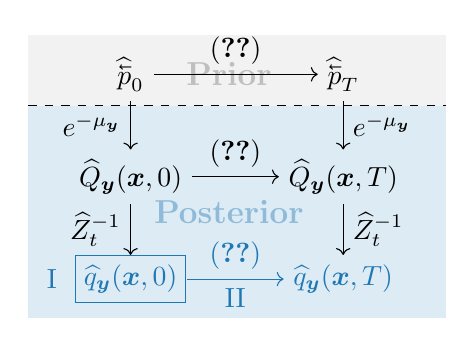
\begin{tikzpicture}
        % Define Seaborn colors
        \definecolor{seabornBlue}{RGB}{31,119,180}

        % Define node positions
        \node (p0) at (0.5,1.3) {$\widehat{\cev{p}}_0$};
        \node (pT) at (3.2,1.3) {$\widehat{\cev{p}}_T$};
        \node (Q0) at (0.5,0) {$\widehat{Q}_{\vy}(\vx, 0)$};
        \node (QT) at (3.2,0) {$\widehat{Q}_{\vy}(\vx, T)$};
        \node[seabornBlue] (q0) at (0.5,-1.3) {$\widehat{q}_{\vy}(\vx, 0)$};
        \node[seabornBlue] (qT) at (3.2,-1.3) {$\widehat{q}_{\vy}(\vx, T)$};

        % Use Seaborn colors for shading
        \begin{scope}[on background layer]
            \fill[gray!10] (-0.8,1.8) rectangle (4.5,0.9);
            \fill[seabornBlue!15] (-0.8,0.9) rectangle (4.5,-1.8);
        \end{scope}
        
        % Draw dashed axes
        \draw[dashed] (-0.8,0.9) -- (4.5,0.9);
        % \draw[dashed] (2.8,3.5) -- (2.8,-0.5);

        % Add labels for quadrants with Seaborn colors
        \node[gray!50] at (1.75,1.3) {\large \textbf{Prior}};
        \node[seabornBlue!50] at (1.75,-0.45) {\large \textbf{Posterior}};

        \draw[->] (p0) -- node[above] {\eqref{eqn: PDE of prior diffusion}} (pT);
        \draw[->] (p0) -- node[left] {$e^{-\mu_\vy}$} (Q0);
        \draw[->] (pT) -- node[right] {$e^{-\mu_\vy}$} (QT);
        \draw[->] (Q0) -- node[above] {\eqref{eqn: PDE of unnormalized posterior diffusion}} (QT);
        \draw[->] (Q0) -- node[left] {$\widehat Z_t^{-1}$} (q0);
        \draw[->] (QT) -- node[right] {$\widehat Z_t^{-1}$} (qT);
        \draw[->, seabornBlue] (q0) -- node[above] {\eqref{eqn: PDE of posterior diffusion}} node[below, seabornBlue] {II} (qT);
        \draw[seabornBlue] (q0) +(-0.7,-0.3) rectangle +(0.7,0.3);
        \node[seabornBlue, left of=q0] {I};
    \end{tikzpicture}
    \caption{A roadmap for our posterior sampling method. I, II refers to the two stages of the proposed algorithm.}
    \vspace{-2.5em}
    \label{fig:commutative diagram for algo derivation}
\end{wrapfigure}

%\vspace{-0.5em}
\subsection{Algorithm Outline}
\label{subsec: algo outline}
%\vspace{-0.5em}

Following the setting in Section~\ref{sec: preliminaries}, we assume the prior distribution $p(\vx)$ is represented by a DM under the EDM framework. Specifically, $p_0(\vx)$ is approximated by $\widehat{\cev{p}}_T(\vx)$, obtained by simulating~\eqref{eqn: EDM SDE} or~\eqref{eqn: EDM PF-ODE} from a Gaussian $\widehat{\cev{p}}_0$. We define the time-dependent posterior distribution as:
\begin{equation}
    \setlength{\abovedisplayskip}{3pt}
    \setlength{\belowdisplayskip}{3pt}
    \label{eqn: defn of time-dependent posterior}
    \widehat{q}_{\vy}(\vx,t) := \frac{\widehat{\cev{p}}_t(\vx)e^{-\mu_{\vy}(\vx)}}{\int_{\mathbb{R}^n}\widehat{\cev{p}}_t(\vx)e^{-\mu_{\vy}(\vx)}\dif\vx} := \frac{\widehat{Q}_{\vy}(\vx,t)}{\widehat{Z}_{\vy}(t)},
\end{equation} 
where $\widehat{Q}_{\vy}(\vx,t)= \widehat{\cev{p}}_t(\vx)e^{-\mu_{\vy}(\vx)}$ is the unnormalized posterior, and $\widehat{Z}_{\vy}(t) = \int_{\mathbb{R}^n}\widehat{Q}_{\vy}(\vx,t)\dif\vx$ is the normalizing constant. 

Our algorithm consists of the following two stages:

%\vspace{-0.5em}
\paragraph{Stage I: Sample from the initial distribution $\widehat{q}_{\vy}(\vx,0)$.}

We first sample from $\widehat{q}_{\vy}(\vx,0) \propto \widehat{\cev{p}}_0(\vx)e^{-\mu_{\vy}(\vx)}$, which is analogous to the likelihood step in~\cite{wu2024principled}. Given differentiable $\mu_{\vy}(\vx)$, we can employ well-known gradient-based samplers like Metropolis Adjusted Langevin Algorithm (MALA)~\cite{roberts2002langevin}, Annealed 
Importance Sampling (AIS)~\cite{neal2001annealed}, or more advanced methods~\cite{lu2019accelerating,tan2023accelerate,chen2024ensemble,lindsey2022ensemble}. For linear BIPs with Gaussian noise, where $\gA:= \mA \in \mathbb{R}^{m \times n}$ and $\vn \sim \gN(\boldsymbol{0},\mSigma)$, assuming $\widehat{\cev{p}}_0 = \gN(\vzero, \rho^2\mI_n)$, the initial distribution simplifies to:
\begin{equation*}
    \setlength{\abovedisplayskip}{3pt}
    \setlength{\belowdisplayskip}{3pt}
    \widehat{q}_{\vy}(\vx,0) \propto \exp\left(-(\vy - \mA\vx)^\intercal\mSigma^{-1}(\vy -\mA\vx)-\tfrac{1}{2\rho^2}\|\vx\|_2^2\right) = \gN(\vgamma, \mLambda^{-1}),   
\end{equation*}
where $\mLambda = \mA^\intercal\mSigma^{-1}\mA+\frac{1}{\rho^2}\mI_n$ and $\vgamma = \mLambda^{-1}\mA^\intercal\mSigma^{-1}\vy$. 
% We remark that our first step here is analogous to the likelihood step in~\cite{wu2024principled}.

%\vspace{-0.5em}
\paragraph{Stage II: Solve the PDE dynamics governing the posterior evolution.}

Below we first derive the PDE dynamics $(\widehat{Q}_{\vy}(\vx,t))_{t\in[0, T]}$ based on the diffusion process~\eqref{eqn: backward sde in standard dm} from $(\widehat{\cev{p}}_t)_{t\in[0, T]}$. Then normalizing these dynamics yields the PDE that evolves $(\widehat{q}_{\vy}(\vx,t))_{t\in[0, T]}$, as illustrated in Figure~\ref{fig:commutative diagram for algo derivation}. 

\begin{enumerate}[leftmargin=*, topsep=0pt, itemsep=2pt, wide]
    \item The Fokker-Planck equation evolving from $\widehat{\cev{p}}_0$ to $\widehat{\cev{p}}_T$ is:
    \begin{equation}
        \setlength{\abovedisplayskip}{3pt}
        \setlength{\belowdisplayskip}{3pt}
        \label{eqn: PDE of prior diffusion}
        \frac{\partial}{\partial t}\widehat{\cev{p}}_t = -\nabla_{\vx} \cdot \left(\left(-F(t)\vx + \tfrac{G(t)^2 + V(t)^2}{2} \vphi_\theta(\vx,t)\right)\widehat{\cev{p}}_t\right) + \tfrac{1}{2}V(t)^2\Delta_{\vx}\widehat{\cev{p}}_t.
    \end{equation}
    
    \item Substituting $\widehat{\cev{p}}_t(\vx) = \widehat{Q}_{\vy}(\vx,t)\exp(\mu_{\vy})$ into \eqref{eqn: PDE of prior diffusion} yields:
    \begin{equation}
        \setlength{\abovedisplayskip}{3pt}
        \setlength{\belowdisplayskip}{3pt}
        \label{eqn: PDE of unnormalized posterior diffusion}
        \begin{aligned}
        \frac{\partial}{\partial t}\widehat{Q}_{\vy} = &-\nabla_{\vx} \cdot \left(\left(\widehat{\mH}(\vx,t)-V(t)^2\nabla_{\vx}\mu_{\vy}\right)\widehat{Q}_{\vy}\right)
        +\tfrac{1}{2}V(t)^2\Delta_{x}\widehat{Q}_{\vy}\\
        &+\left(\tfrac{1}{2}V(t)^2\left(\|\nabla_{\vx}\mu_{\vy}\|_2^2-\Delta_{\vx}\mu_{\vy}\right) - \widehat{\mH}(\vx,t)^\intercal\nabla_{\vx}\mu_{\vy}\right)\widehat{Q}_{\vy},
        \end{aligned}    
    \end{equation}
    where $\widehat{\mH}(\vx,t) := -F(t)\vx + \frac{G(t)^2 + V(t)^2}{2} \vphi_\theta(\vx,t)$ is the original drift. A complete derivation of~\eqref{eqn: PDE of unnormalized posterior diffusion} is postponed to Lemma~\ref{lem: simplifying dynamics} in Appendix~\ref{sec: derivations for Sec 3}.
    
    \item Defining $U(\vx, t) := \frac{1}{2}V(t)^2\left(\|\nabla_{\vx}\mu_{\vy}\|_2^2-\Delta_{\vx}\mu_{\vy}\right)$, we have the following PDE for $\widehat{q}_{\vy}(\vx,t)$:
    \begin{tcolorbox}[colback=lightgray,boxrule=0pt,sharp corners]
        %\vspace{-0.3em}
        \underline{\bfseries PDE Dynamics for Posterior Evolution}
        \begin{equation}
            \setlength{\abovedisplayskip}{3pt}
            \setlength{\belowdisplayskip}{3pt}
            \label{eqn: PDE of posterior diffusion}
            \begin{aligned}
            \frac{\partial}{\partial t}&\widehat{q}_{\vy} = -\nabla_{\vx} \cdot \left(\left(\widehat{\mH}(\vx,t)-V(t)^2\nabla_{\vx}\mu_{\vy}\right)\widehat{q}_{\vy}\right)
            +\tfrac{1}{2}V(t)^2\Delta_{x}\widehat{q}_{\vy}\\
            &+\left(U(\vx,t) - \widehat{\mH}(\vx,t)^\intercal\nabla_{\vx}\mu_{\vy} - \int_{\mathbb{R}^n}\left(U(\vx,t) - \widehat{\mH}(\vx,t)^\intercal\nabla_{\vx}\mu_{\vy}\right)\widehat{q}_{\vy}\dif \vx\right)\widehat{q}_{\vy}.
            \end{aligned}
        \end{equation}
        % %\vspace{-1.0em}
    \end{tcolorbox}
    This derivation involves averaging the linear term in~\eqref{eqn: PDE of unnormalized posterior diffusion}, a technique used in recent works~\cite{skreta2025feynman,lee2025debiasing,holderrieth2025leaps}. For a complete proof one may refer to Lemma~\ref{lem: normalizing linear term in dynamics} in Appendix~\ref{sec: derivations for Sec 3}.
\end{enumerate}

%\begin{remark}
%\label{rmk: derivation of true dynamics}
%By replacing $\vphi_{\theta}(\vx,t)$ and $\widehat{\mH}(\vx,t)$ with $\nabla\log\cev{p}_{t}(\vx)$ and $H(\vx,t):=-F(t)\vx + \frac{G(t)^2+V(t)^2}{2}\nabla\log\cev{p}_{t}(\vx)$ respectively, we can perform the derivation of the PDE dynamics~\eqref{eqn: PDE of prior diffusion},~\eqref{eqn: PDE of unnormalized posterior diffusion} and~\eqref{eqn: PDE of posterior diffusion} in exactly the same way to obtain new PDE dynamics associated with the true score function. Though these dynamics can not lead to algorithms we used in practice, they will be useful for the theoretical analysis conducted in subsection~\ref{subsec: error bound btween posterior in terms of prior} later on. 
%\end{remark}

%\vspace{-0.5em}
\subsection{Posterior Sampling via Weighted Particles}
\label{subsection: algorithm details}
%\vspace{-0.5em}

We now present two ensemble-based posterior samplers within the SMC framework, which can also be interpreted as solving the PDE~\eqref{eqn: PDE of posterior diffusion} numerically via (stochastic) weighted particles.

\paragraph{(Stochastic) Weighted Particle / Sequential Monte Carlo Methods.}

As shown in Lemma~\ref{lem: derivation of single particle dynamics} of Appendix~\ref{sec: derivations for Sec 3}, the posterior evolution~\eqref{eqn: PDE of posterior diffusion} can be simulated via the following dynamics of a single weighted particle  $(\vx_t,\beta_t)$:
\begin{equation}
    \setlength{\abovedisplayskip}{3pt}
    \setlength{\belowdisplayskip}{3pt}
    \label{eqn: PDE soln via single particle} 
    \begin{cases}
    \dif \vx_t &= \left(\widehat{\mH}(\vx_t,t)-V(t)^2\nabla_{\vx}\mu_{\vy}(\vx_t)\right)\dif t + V(t)\dif \vw_t,\\
    \dif \beta_t &= \left(U(\vx_t,t) - \widehat{\mH}(\vx_t,t)^\intercal\nabla_{\vx}\mu_{\vy}(\vx_t)\right)\beta_t \dif t \\
    &- \left(\displaystyle\int_{\mathbb{R}^n}\left(U(\vx,t) - \widehat{\mH}(\vx,t)^\intercal\nabla_{\vx}\mu_{\vy}(\vx)\right)\left(P_{\beta}\gamma_t\right)(\vx)\dif \vx\right)\beta_t \dif t,    
    \end{cases}
\end{equation}
where $\gamma_t(\vx,\beta)$ denotes the joint probability distribution of $(\vx_t,\beta_t)$ and $P_{\beta}\gamma_t(\vx) := \int_{\mathbb{R}}\beta\gamma_t(\vx,\beta)\dif \beta$ denotes the weighted projection of $\gamma_t$ onto $\vx$. To effectively approximate the integral in $P_\beta \gamma_t$, we then use the empirical measure $\gamma_t(\vx,\beta) \approx \frac{1}{N}\sum_{i=1}^{N}\delta_{(\vx^{(i)}_t,\beta^{(i)}_t)}$ formed by $N$ weighted particles to approximate $\gamma_t(\vx,\beta)$. This leads to the following joint dynamics for $\{(\vx^{(i)}_t, \beta^{(i)}_t)\}_{i=1}^{N}$:
\begin{tcolorbox}[colback=lightgray,boxrule=0pt,sharp corners]
    %\vspace{-0.3em}
    \underline{\bfseries Weighted Particle Dynamics for Posterior Evolution}
    %\vspace{-0.5em}
    \begin{equation}
    \label{eqn: PDE soln via ensemble of particles} 
    \begin{cases}
    \dif \vx^{(i)}_t &= \left(\widehat{\mH}(\vx^{(i)}_t,t)-V(t)^2\nabla_{\vx}\mu_{\vy}(\vx^{(i)}_t)\right)\dif t + V(t)\dif \vw^{(i)}_t,\\
    \dif \beta^{(i)}_t &= \left(U(\vx^{(i)}_t,t) - \widehat{\mH}(\vx^{(i)}_t,t)^\intercal\nabla_{\vx}\mu_{\vy}(\vx^{(i)}_t)\right)\beta^{(i)}_t \dif t \\
    &- \left(\frac{1}{N}\sum_{j=1}^{N}\left(U(\vx^{(j)}_t,t) - \widehat{\mH}(\vx^{(j)}_t,t)^\intercal\nabla_{\vx}\mu_{\vy}(\vx^{(j)}_t)\right)\beta^{(j)}_t\right)\beta^{(i)}_t \dif t,  
    \end{cases}
    \end{equation}
    %\vspace{-1.0em}
\end{tcolorbox}
with initial conditions $\vx^{(i)}_0 \sim \widehat{q}_{\vy}(\cdot,0)$ and $\beta^{(i)}_0 = 1$, for $i \in [N]$. The weighted projection equals $\frac{1}{N}\beta^{(j)}_t$ when $\vx = \vx^{(j)}_t$ for some $j$, and zero otherwise.

\IncMargin{1.5em}
% \begin{wrapfigure}{r}{0.53\textwidth}
    %\vspace{-1.5em}
    \begin{algorithm}[t]
        \caption{Resampling Step}
        \label{alg:resampling}
        \Indm
        \KwIn{Threshold $c \in (0,1)$, weighted particles $\{(\vx^{(j)}, \beta^{(j)})\}_{j=1}^{N}$}
        \KwOut{Updated particles $\{(\widehat{\vx}^{(j)}, \widehat{\beta}^{(j)})\}_{j=1}^{N}$}
        \Indp
        \uIf{$\text{ESS} = \frac{\left(N^{-1}\sum_{j=1}^{N}\beta^{(j)}\right)^2}{N^{-1}\sum_{j=1}^{N}(\beta^{(j)})^2}< c$}{
        Sample $\{\widehat{\vx}^{(j)}\}_{j=1}^{N}$ with replacement from $\{\vx^{(j)}\}_{j=1}^{N}$ with probability \small$\left\{\frac{\beta^{(j)}}{\sum_{i=1}^{N}\beta^{(i)}}\right\}_{j=1}^N$\;
        $\widehat{\beta}^{(j)} \leftarrow 1$, for $j \in [N]$\;
        }
        \Else{
        $\{(\widehat{\vx}^{(j)}, \widehat{\beta}^{(j)})\}_{j=1}^{N} \leftarrow \{(\vx^{(j)}, \beta^{(j)})\}_{j=1}^{N}$\;
        }
    \end{algorithm}
    %\vspace{-2.0em}
% \end{wrapfigure}

While numerical discretization of~\eqref{eqn: PDE soln via ensemble of particles} yields a prototypical sampling algorithm, the particle weights $\beta^{(i)}_t$ may diverge during simulation, reducing the ensemble's Effective Sample Size (ESS). To address this, we employ a resampling strategy commonly used in the SMC methods~\cite{liu2001monte,chopin2002sequential,del2006sequential,doucet2009tutorial,del2013mean,moral2004feynman}, whose detailed description is provided in Algorithm~\ref{alg:resampling}. Such resampling sub-routine essentially performs global moves by eliminating low-weight particles and duplicating high-weight ones, similar to the birth-death process used in~\cite{moral2004feynman,lu2019accelerating,tan2023accelerate,chen2024ensemble,lindsey2022ensemble}. However, the resampling approach is computationally more efficient as the weight dynamics~\eqref{eqn: PDE soln via ensemble of particles} can be parallelized.


\paragraph{SDE Approach (AFDPS-SDE).}

We first consider the SDE implementation~\eqref{eqn: EDM SDE} of the diffusion model, where $V(t) = G(t) = s(t)\sqrt{2\dot{\sigma}(t)\sigma(t)}$. We directly discretize~\eqref{eqn: PDE soln via ensemble of particles} with an Euler-Maruyama scheme and add Algorithm~\ref{alg:resampling} as an adjustment step at the end of each iteration, which leads to Algorithm~\ref{alg:sde}. We have omitted the averaging term, \emph{i.e.}, the last line of~\eqref{eqn: PDE soln via ensemble of particles} in Algorithm~\ref{alg:sde}, in practical implementation since the update is the same for all particles and therefore cancels out when we normalize the weights. Such cancellation property also holds for the ODE approach presented below. For high-dimensional problems, we can further reduce the computational cost of both the SDE and the ODE approach via practical techniques like using a smaller ensemble, omitting the resampling step, and simply returning the particle with the highest weight as the best estimator, as discussed in Appendix~\ref{sec: implementation detail app}.  

%$V(t) = G(t) = s(t)\sqrt{2\dot{\sigma}(t)\sigma(t)}$ function our algorithms might also need to be modified accordingly. For SDE one can directly obtain %We note that Algorithm 1~\ref{alg:resampling} essentially  can also be implemented via the birth death process used in~\cite{lu2019accelerating,tan2023accelerate,chen2024ensemble,lindsey2022ensemble} in~\eqref{eqn: PDE soln via ensemble of particles},  For high-dimensional problems with high computational cost, we may also keep an ensemble of moderate we can also save for largest weight only,Note that, which helps us save computational cost. also can retur just one, implement in parallel ,

% \IncMargin{1.5em}
\setlength{\textfloatsep}{10pt} 
\begin{algorithm}[!t]
    \caption{Approximation-Free Diffusion Posterior Sampler via SDE (AFDPS-SDE)}
    \label{alg:sde}
    \Indm
    \KwIn{Noisy observation $\vy$, log-likelihood $\mu_{\vy}(\cdot)$, functions $s(t)$ and $\sigma(t)$, time grid $\{t_i\}_{i=0}^{K}$ with $t_0 = 0$ and $t_K = T$, thresholds $\{c_l\}_{l=1}^{K}$, score function $\vphi_\theta(\cdot,t)$, ensemble size $N$, initial weights $\beta^{(j)}_0 = 1$ for $j\in[N]$.}
    \KwOut{Posterior approximation $\sum_{j=1}^{N}\beta^{(j)}_T \delta_{\vx^{(j)}_T}/\sum_{j=1}^{N}\beta^{(j)}_T$.}
    \Indp
    Draw $\{\vx^{(i)}_{0}\}_{i=1}^{N}$ i.i.d. from $\widehat{q}_{\vy}(\cdot,0)$ via Stage I samplers in Section~\ref{subsec: algo outline}\;
    \For{$k = 0$ \KwTo $K-1$}{
    Draw $\{\xi^{(j)}_{k}\}_{j=1}^{N}$ i.i.d. from $\gN(\boldsymbol{0},\mI_n)$\;
        \For{$j = 1$ \KwTo $N$}{\small
        $\begin{aligned}
            \widehat{\vx}^{(j)}_{t_{k+1}} &\leftarrow \left(1-(t_{k+1}-t_k)\tfrac{\dot{s}(t_k)}{s(t_k)}\right)\vx^{(j)}_{t_{k}} + s(t_k)\sqrt{2\dot{\sigma}(t_k)\sigma(t_k)(t_{k+1}-t_k)}\xi^{(j)}_{k}\\ 
            &+ 2(t_{k+1}-t_k)s(t_k)^2\dot{\sigma}(t_k)\sigma(t_k)\left(\vphi_{\theta}(\vx^{(j)}_{t_k},t_k) -\nabla_{\vx}\mu_{\vy}(\vx^{(j)}_{t_k})\right);
        \end{aligned}$

        $\begin{aligned}
            \log\widehat{\beta}^{(j)}_{t_{k+1}} &\leftarrow \log\beta^{(j)}_{t_{k+1}} +(t_{k+1}-t_k)\tfrac{\dot{s}(t_k)}{s(t_k)}\nabla_{\vx}\mu_{\vy}(\vx^{(j)}_{t_k})^\intercal \vx^{(j)}_{t_k}\\
            &-2(t_{k+1}-t_k)s(t_k)^2\dot{\sigma}(t_k)\sigma(t_k)\nabla_{\vx}\mu_{\vy}(\vx^{(j)}_{t_k})^\intercal\vphi_{\theta}(\vx^{(j)}_{t_k},t_k)\\
            &+ (t_{k+1} - t_k)s(t_k)^2\dot{\sigma}(t_k)\sigma(t_k)\left(\|\nabla_{\vx}\mu_{\vy}(\vx^{(j)}_{t_k})\|_2^2-\Delta_{\vx}\mu_{\vy}(\vx^{(j)}_{t_k})\right);
        \end{aligned}$
        }
    {\small$\{(\vx^{(j)}_{t_{k+1}},\beta^{(j)}_{t_{k+1}})\}_{j=1}^{N} \leftarrow$ Algorithm~\ref{alg:resampling}$\left(c_{k+1},\{(\widehat{\vx}^{(j)}_{t_{k+1}},\widehat{\beta}^{(j)}_{t_{k+1}})\}_{j=1}^{N}\right)$\;}
    }
\end{algorithm}

\paragraph{ODE+Corrector Approach (AFDPS-ODE).}

% \begin{wrapfigure}{r}{0.5\textwidth}
    %\vspace{-1.5 em}
    \begin{algorithm}[t]
        \caption{Corrector Step}
        \label{alg:corrector}
        \Indm
        \KwIn{Initialization $\widehat{x}_0$, time $t$, iterations $L$, stepsize $h$, log-likelihood $\mu_{\vy}(\cdot)$, score function $\vphi_{\theta}(\cdot)$.}
        \KwOut{Sample $\widehat{x}_{L} \sim \widehat{q}_{\vy}(\vx,t) \propto \widehat{\cev{p}}_t(\vx)\exp(-\mu_{\vy}(\vx))$.}
        \Indp
        Draw $\left\{\xi_{l}\right\}_{l=1}^{L}$ i.i.d. from $\gN(\boldsymbol{0},\mI_n)$\;
        \For{$l = 0$ \KwTo $L-1$}{
            $\widehat{\vx}_{l+1} \leftarrow \widehat{\vx}_{l} + h\left(\vphi_{\theta}(\widehat{\vx}_l,t)-\nabla_{\vx}\mu_{\vy}(\widehat{\vx}_{l})\right) + \sqrt{2h}\xi_{l+1};$
        }
    \end{algorithm}
    %\vspace{-1.5em}
% \end{wrapfigure}

Next, we consider an alternative implementation based on the probability flow ODE~\eqref{eqn: EDM PF-ODE} by setting $V(t)=0$. While this leads to the ODE dynamics~\eqref{eqn: PDE soln via ensemble of particles}, relying solely on deterministic evolution may not sufficiently explore the target distribution. To enhance exploration, we incorporate a stochastic corrector step inspired by predictor-corrector schemes in diffusion models~\cite{song2020score,chen2024probability,bradley2024classifier}. The corrector uses the Unadjusted Langevin Algorithm (ULA, Algorithm~\ref{alg:corrector}) to draw samples from the intermediate posterior distribution $\widehat{q}_{\vy}(\vx,t) \propto \widehat{\cev{p}}_t(\vx)\exp(-\mu_{\vy}(\vx))$ at each timestep. The complete ODE+Corrector algorithm (Algorithm~\ref{alg:edm pf-ode + corrector}) is thus obtained by discretizing the probability flow ODE~\eqref{eqn: PDE soln via ensemble of particles}, and applying both resampling (Algorithm~\ref{alg:resampling}) and ULA correction (Algorithm~\ref{alg:corrector}) steps for adjustments.

%\vspace{-.45em}
\begin{remark}[Connection with Feynman-Kac corrector~\cite{skreta2025feynman} and Guidance~\cite{dhariwal2021diffusion,bradley2024classifier}]

    A recent work~\cite{skreta2025feynman} proposed a related ensemble-based sampler within the SMC framework. However, the dynamics derived in our setting differ from those in Proposition~D.5 of~\cite{skreta2025feynman}, which is essentially the ODE case without correctors in our method. The key difference is the presence of a gradient term, $\nabla_{\vx}\mu_{\vy}$, in the dynamics of $\vx_t$~\eqref{eqn: PDE soln via single particle}, which is absent in their formulation. Such component, previously used in SGS + DM methods~\cite{xu2024provably,wu2024principled} and in optimization-based denoising algorithms such as ADMM~\cite{gabay1976dual,wang2008new,boyd2011distributed,sun2016deep,chan2016plug,ryu2019plug} and FISTA~\cite{beck2009fast,zhang2018ista,xiang2021fista}, is incorporated into our DM-based framework in a systematic way. The derivation illustrated in Figure~\ref{fig:commutative diagram for algo derivation} is shown to be essential for the method's empirical performance (\emph{cf.}~Section~\ref{sec: results of numerics}). A detailed comparison is given in Remark~\ref{rmk: difference between our dynamics and FK corrector} of Appendix~\ref{sec: derivations for Sec 3}.

    In contrast to prior work on guided diffusion sampling~\cite{dhariwal2021diffusion,bradley2024classifier,wu2024theoretical,chidambaram2024does} and its extensions~\cite{ho2022classifier,bansal2023universal,song2023loss,he2023manifold,guo2024gradient,lu2024guidance,zheng2024ensemble,ye2024tfg}, which augment single-particle dynamics with a gradient term such as $\nabla_\vx\log p_{t}(\vy|\vx_t)$ or $\nabla_\vx\log p_{t}(\vx_t|\vy)$, our PDE-based derivation naturally yields the gradient term $\nabla_{\vx}\mu_{\vy}$ within a principled framework. Additionally, our formulation introduces a linear term that must be simulated via an ensemble of weighted particles, rather than from a single trajectory. Such ensemble-based structure allows us to integrate gradient-based guidance and diffusion sampling under the SMC framework in a unified way, resulting in improved empirical performance.
\end{remark}

\begin{algorithm}[!t]
    \caption{Approx.-Free Diffusion Posterior Sampler via ODE+Corrector (AFDPS-ODE)}
    \label{alg:edm pf-ode + corrector}
    \Indm
    \KwIn{Noisy observation $\vy$, log-likelihood $\mu_{\vy}(\cdot)$, functions $s(t)$ and $\sigma(t)$, time grid $\{t_i\}_{i=0}^{K}$ with $t_0 = 0$ and $t_K = T$, thresholds $\{c_l\}_{l=1}^{K}$, score function $\vphi_\theta(\cdot,t)$, corrector iterations $n_c$, stepsize $h_c$, ensemble size $N$, initial weights $\beta^{(j)}_0 = 1$ for $j\in[N]$.}
    \KwOut{Posterior approximation $\sum_{j=1}^{N}\beta^{(j)}_T\delta_{\vx^{(j)}_T}/\sum_{j=1}^{N}\beta^{(j)}_T$.}
    \Indp
    Draw $\{\vx^{(i)}_{0}\}_{i=1}^{N}$ i.i.d. from $\widehat{q}_{\vy}(\cdot,0)$ via Stage I samplers in Section~\ref{subsec: algo outline}\;
    \For{$k = 0$ \KwTo $K-1$}{
        \For{$j = 1$ \KwTo $N$}{
            \small$\widetilde{\vx}^{(j)}_{t_{k+1}} \leftarrow \left(1-(t_{k+1}-t_k)\frac{\dot{s}(t_k)}{s(t_k)}\right)\vx^{(j)}_{t_{k}} + (t_{k+1}-t_k)s(t_k)^2\dot{\sigma}(t_k)\sigma(t_k)\vphi_{\theta}(\vx^{(j)}_{t_k},t_k)$\;
            $\widehat{\vx}^{(j)}_{t_{k+1}} \leftarrow \text{Algorithm}~\ref{alg:corrector}\left(\widetilde{\vx}^{(j)}_{t_{k+1}},t_{k+1},n_c,h_c, \mu_{\vy}(\cdot),\vphi_\theta(\cdot,t)\right)$\;
            $\begin{aligned}
                \log\widehat{\beta}^{(j)}_{t_{k+1}} \leftarrow \log\beta^{(j)}_{t_{k+1}} &+(t_{k+1}-t_k)\tfrac{\dot{s}(t_k)}{s(t_k)}\nabla_{\vx}\mu_{\vy}\left(\vx^{(j)}_{t_k}\right)^\intercal \vx^{(j)}_{t_k}\\
                &-(t_{k+1}-t_k)s(t_k)^2\dot{\sigma}(t_k)\sigma(t_k)\nabla_{\vx}\mu_{\vy}\left(\vx^{(j)}_{t_k}\right)^\intercal\vphi_{\theta}\left(\vx^{(j)}_{t_k},t_k\right);
            \end{aligned}$
        }
        {\small$\{(\vx^{(j)}_{t_{k+1}},\beta^{(j)}_{t_{k+1}})\}_{j=1}^{N} \leftarrow$ Algorithm~\ref{alg:resampling}$\left(c_{k+1},\{(\widehat{\vx}^{(j)}_{t_{k+1}},\widehat{\beta}^{(j)}_{t_{k+1}})\}_{j=1}^{N}\right)$\;}
    }
\end{algorithm}



\section{Theoretical Analysis}
\label{sec: main result - theory}

In this section, we present our theoretical results of the ensemble-based posterior samplers introduced in Section~\ref{sec: main result - algorithms}. Our analysis is conducted in continuous time, based on the weighted particle dynamics~\eqref{eqn: PDE of posterior diffusion} and~\eqref{eqn: PDE soln via ensemble of particles}. The impact of numerical discretization, as implemented in Algorithm~\ref{alg:sde} and Algorithm~\ref{alg:edm pf-ode + corrector}, is not considered here and is left for future work. Without loss of generality, we focus on the backward SDE setting~\eqref{eqn: EDM SDE}, specifically using $s(t)=1$ and $\sigma(t)=t$. We begin by introducing several technical assumptions.

\begin{assumption}[Regularity of the log-likelihood]
\label{assump: regularity and boundedness of log-likelihood}
The log-likelihood function $\mu_{\vy}$ is twice differentiable and lower bounded by some constant $C^{(1)}_{\vy}$  depending only on the observation $\vy$.     
\end{assumption}


\begin{assumption}[Bounded second moment]
\label{assump: bounded second moment}
The prior distribution $p_0$ satisfies a second-moment bound: $\mathbb{E}{p_0}\left[\|\vx\|_{2}^2\right] \leq m_2^2$.
\end{assumption}


\begin{assumption}[Score matching error]
\label{assump: score matching training error}
The neural network estimator $\vphi_{\theta}(\vx,t)$ approximates the score function $\nabla_{\vx}\log \cev{p}_t(\vx)$ with uniformly bounded error across $t \in [0,T]$:
$$
    \int_{\mathbb{R}^n}\left\|\vphi_{\theta}(\vx,t)-\nabla_{\vx}\log \cev{p}_{t}(\vx)\right\|_{2}^2\cev{p}_t(\vx)\dif \vx  \leq \epsilon_{\vs}^2.
$$
\end{assumption}

Assumption~\ref{assump: regularity and boundedness of log-likelihood} ensures the absence of singularities in the log-likelihood $\mu_{\vy}$, which is a condition  adopted in existing work on BIPs~\cite{stuart2010inverse} and satisfied by common noise models such as Gaussian and Poisson (with $C^{(1)}_{\vy} = 0$). Assumptions~\ref{assump: bounded second moment} and~\ref{assump: score matching training error} are aligned with recent theoretical frameworks for diffusion models~\cite{wang2024evaluating,chen2022sampling,chen2023improved,benton2023linear,chen2024probability}. Particularly, Assumption~\ref{assump: score matching training error} quantifies the approximation error due to neural network training and reflects the quality of the pre-trained score function.

We now present our first main result, which quantifies the discrepancy between the true posterior $q_{\vy,0}$ and the distribution $\widehat{q}_{\vy,T}$ obtained by evolving our derived PDE dynamics~\eqref{eqn: PDE of posterior diffusion} for time $T$.

\begin{tcolorbox}[colback=lightgray,boxrule=0pt,sharp corners]
\begin{theorem}[Error Bound for Posterior Estimation]
\label{thm: bound on true and approx posterior}
Under Assumptions~\ref{assump: regularity and boundedness of log-likelihood}, \ref{assump: bounded second moment}, and \ref{assump: score matching training error}, the total variation (TV) distance between the approximate and true posterior satisfies:
$$
    \TV(\widehat{q}_{\vy,T},q_{\vy,0}) \leq C^{(2)}_{\vy}\sqrt{\frac{m_2^2}{T^2} + T^2\epsilon_{\vs}^2}
$$
where $q_{\vy,0}(\vx) \propto p_0(\vx)\exp(-\mu_{\vy}(\vx))$ is the exact posterior, and $\widehat{q}_{\vy,t}$ is the solution to the posterior evolution~\eqref{eqn: PDE of posterior diffusion}. The constant $C^{(2)}_{\vy}$ depends only on the observation $\vy$. Optimizing the right-hand side yields the asymptotic bound $\TV(\widehat{q}_{\vy,T},q_{\vy,0}) \lesssim \sqrt{\epsilon_\vs}$ when $T \asymp \sqrt{\epsilon_\vs^{-1}}$.
\end{theorem}
\end{tcolorbox}

A detailed proof of Theorem~\ref{thm: bound on true and approx posterior} can be found in Section~\ref{proof: posterior bound by prior error}. It essentially combines techniques from the theory of diffusion models~\cite{chen2023improved,wang2024evaluating} and the well-posedness theory of Bayesian inverse problems, which is closely related to~\cite[Theorem 4.1]{purohit2024posterior}. The result of Theorem~\ref{thm: bound on true and approx posterior} reveals a trade-off controlled by the time horizon $T$ between the prior mismatch and score approximation error.

Next, we study the particle approximation to the PDE solution~\eqref{eqn: PDE of posterior diffusion}. In particular, we examine the convergence of the dynamics of the weighted particle ensemble~\eqref{eqn: PDE soln via ensemble of particles} in the many-particle limit.

\begin{assumption}[Boundedness and Lipschitz continuity of $I$]
\label{assump: boundedness and Lipschitz of I}
Define the function
$$
    I(\vx,t):=\|\nabla_{\vx}\mu_{\vy}(\vx)\|_2^2 - \Delta_{\vx}\mu_{\vy}(\vx)-2\vphi_{\theta}(\vx,t)^\intercal\nabla_{\vx}\mu_{\vy}(\vx).
$$
We assume that $I(\vx,t)$ is uniformly bounded and Lipschitz continuous over $\mathbb{R}^n \times [0,T]$:
$\max\{\|I\|_{L^{\infty}(\mathbb{R}^n \times [0,T])},\mathrm{Lip}(I)\} \leq B_{\vy}$,
for some constant $B_{\vy}$ depending only on $\vy$.
\end{assumption}

Assumption~\ref{assump: boundedness and Lipschitz of I} ensures stability of the evolving particle weights, preventing degeneracy or explosion over time. In practice, this condition is enforced via the resampling step in Algorithm~\ref{alg:resampling}. While we adopt this assumption for analytical tractability, relaxing it and developing a rigorous theory of the resampling step remain important future directions, which might link to existing theoretical studies~\cite{lu2023birth,chen2023sampling,yan2024learning} on sampling algorithms that use birth-death dynamics or Fisher–Rao gradient flow.

\begin{tcolorbox}[colback=lightgray,boxrule=0pt,sharp corners]
\begin{theorem}[Convergence in the Many-Particle Limit]
\label{thm: many-particle limit}
Under Assumptions~\ref{assump: regularity and boundedness of log-likelihood}–\ref{assump: boundedness and Lipschitz of I}, the empirical distribution of the particle system converges to the solution of the posterior PDE. Specifically, for all $t \in [0,T]$,
$$\lim_{N \rightarrow \infty}\mathbb{E}[\gW^2_2(\gamma^{N}_{t}, \gamma_{t})] = 0,$$
where $\gamma_t$ is the law of a single weighted particle pair $(\vx_t, \beta_t)$ governed by~\eqref{eqn: PDE soln via single particle}, such that the marginal $\widehat{q}_{\vy}(\cdot,t)$ is recovered via $P_{\beta}\gamma_t(\cdot) = \int_{\mathbb{R}}\beta\gamma_t(\cdot,\beta)\dif\beta = \widehat{q}_{\vy}(\cdot,t)$, and $\gamma^{N}_{t}$ is the empirical measure of the $N$-particle system $\left\{\left(\vx^{(i)}_t, \beta^{(i)}_t\right)\right\}_{i=1}^N$ governed by~\eqref{eqn: PDE soln via ensemble of particles}.
% Here,
\end{theorem}
\end{tcolorbox}

Theorem~\ref{thm: many-particle limit} establishes the mean-field consistency of the weighted ensemble approximation in the 2-Wasserstein sense. Its proof, which is presented in Appendix~\ref{proof: mean-field limit}, is based on results from propagation of chaos~\cite{sznitman1991topics,lacker2018mean}. Together with Theorem~\ref{thm: bound on true and approx posterior}, our theoretical results provide both rigorous guarantee for the accuracy of the continuum posterior approximation and justification of the proposed ensemble-based implementation.


%\subsection{Error bound between posterior in terms of prior}
%\label{subsec: error bound btween posterior in terms of prior}
%\subsection{Mean Field Limit for SDE/ODE Implementations}
%\subsection{Asymptotic Convergence of Backward ODE and SDE Under the Many-Particle Limit}

%In this subsection, state the . convergence of wasserstein-2 distance; %Error Bound 2: mean field limit of ensemble of particles; just  to obtain convergence in Wasserstein-2 distance (positions and weights)

%\vspace{-.5em}
\section{Experiments}
\label{sec: results of numerics}
%\vspace{-.5em}

In this section, we evaluate the empirical performance of our method on several BIPs in imaging. Additional implementation details and experimental results can be found in Appendix~\ref{sec: implementation detail app} and~\ref{sec: experiment results detail app}, respectively. 

%\vspace{-.5em}
\paragraph{Problem Setting.}

We consider four canonical inverse problems: Gaussian Deblurring (GD), Motion Deblurring (MD), Super Resolution (SR), and Box Inpaint (BI). In all these tasks, we assume that the observational noise is isotropic Gaussian with variance $0.2$, \emph{i.e.}, $\vn \sim \gN(\vzero, 0.2 \mI_m)$ in~\eqref{eqn: BIP setup}, a more challenging setting compared to the commonly used low-noise scenario with variance $2.5 \times 10^{-3}~$\cite{dou2024diffusion,wu2024principled}. Experiments are conducted on FFHQ-256~\cite{karras2019style} and ImageNet-256~\cite{deng2009imagenet}, two widely used datasets in imaging and vision.

%\vspace{-.5em}
\paragraph{Baselines.}

We compare our proposed algorithms with several state-of-the-art diffusion model-based posterior sampling methods:
\begin{itemize}[leftmargin=1.5em, itemsep=0pt, topsep=0pt, parsep=0pt]
    \item \emph{DPS~\cite{chung2022diffusion}}: a sampler that guides the pretrained DM with approximations of manifold-constrained gradients derived from the measurement likelihood.
    \item \emph{DCDP~\cite{li2024decoupled}}: a framework alternating between optimization steps that ensure data consistency and pretrained DMs for posterior sampling.
    \item \emph{SGS-EDM~\cite{wu2024principled}}: a split Gibbs sampler coupled with a DM for efficient posterior inference.
    \item \emph{FK-Corrector~\cite{skreta2025feynman}}: an SMC-based sampler using Feynman-Kac formula to correct trajectories.
    \item \emph{PF-SMC-DM~\cite{dou2024diffusion}}: a particle filtering framework combining SMC with diffusion models.
\end{itemize}

\begin{wrapfigure}{r}{0.42\textwidth}
    \vspace{-1.2em}
    \centering
    % First row
    \begin{subfigure}[b]{0.11\textwidth}
        \includegraphics[width=\linewidth]{figures/ffhq_gblur_gt.png}
    \end{subfigure}%
    \begin{subfigure}[b]{0.11\textwidth}
        \includegraphics[width=\linewidth]{figures/ffhq_sr_gt.png}
    \end{subfigure}%
    \begin{subfigure}[b]{0.11\textwidth}
        \includegraphics[width=\linewidth]{figures/imagenet_gblur_gt.png}
    \end{subfigure}%
    \begin{subfigure}[b]{0.11\textwidth}
        \includegraphics[width=\linewidth]{figures/imagenet_sr_gt.png}
    \end{subfigure}
    
    %\vspace{-0.1\baselineskip}
    
    \begin{subfigure}[b]{0.11\textwidth}
        \includegraphics[width=\linewidth]{figures/ffhq_gblur_meas.png}
    \end{subfigure}%
    \begin{subfigure}[b]{0.11\textwidth}
        \includegraphics[width=\linewidth]{figures/ffhq_sr_meas.png}
    \end{subfigure}%
    \begin{subfigure}[b]{0.11\textwidth}
        \includegraphics[width=\linewidth]{figures/imagenet_gblur_meas.png}
    \end{subfigure}%
    \begin{subfigure}[b]{0.11\textwidth}
        \includegraphics[width=\linewidth]{figures/imagenet_sr_meas.png}
    \end{subfigure}
    
    %\vspace{-0.1\baselineskip}
    
    \begin{subfigure}[b]{0.11\textwidth}
        \includegraphics[width=\linewidth]{figures/ffhq_gblur_recon.png}
    \end{subfigure}%
    \begin{subfigure}[b]{0.11\textwidth}
        \includegraphics[width=\linewidth]{figures/ffhq_sr_recon.png}
    \end{subfigure}%
    \begin{subfigure}[b]{0.11\textwidth}
        \includegraphics[width=\linewidth]{figures/imagenet_gblur_recon.png}
    \end{subfigure}%
    \begin{subfigure}[b]{0.11\textwidth}
        \includegraphics[width=\linewidth]{figures/imagenet_sr_recon.png}
    \end{subfigure}
    \vspace{-.1em}
    \caption{Visualization of posterior samples by AFDPS. \textbf{Upper:} Original; \textbf{Middle:} Blurred; \textbf{Lower:} Reconstructed.}
    \label{fig:2x4compact}
    \vspace{-1.5em}
\end{wrapfigure}

%\vspace{-.5em}
\paragraph{Experimental Settings.}

To ensure a fair comparison, we use the same checkpoints for the two pre-trained score functions provided in~\cite{chung2022diffusion} and fix the number of function evaluations (NFE) to $2 \times 10^4$ across all methods. For ensemble-based approaches, the number of particles is set to $N = 10$. In the case of AFDPS-ODE (Algorithm~\ref{alg:edm pf-ode + corrector}), we reduce the number of particles to $N = 5$ to offset the additional computational cost from the corrector step, while maintaining the total NFE consistent with AFDPS-SDE (Algorithm~\ref{alg:sde}). We evaluate reconstruction quality using two metrics: PSNR (Peak Signal-to-Noise Ratio), which quantifies pixel-level accuracy, and LPIPS (Learned Perceptual Image Patch Similarity)~\cite{zhang2018unreasonable}, which measures perceptual similarity; both metrics are computed between the reconstructed sample mean and the ground truth image over a set of 100 randomly selected validation images.


{
\begin{table}[htbp]
\centering
\caption{Results on 4 inverse problems for 100 validation images from FFHQ-256.}
\resizebox{\textwidth}{!}{
\begin{tabular}{l|cc|cc|cc|cc}
\noalign{\hrule height 1.2pt} 
\multirow{2}{*}{\bfseries Method} 
& \multicolumn{2}{c|}{\bfseries Gaussian Deblurring}
& \multicolumn{2}{c|}{\bfseries Motion Deblurring}
& \multicolumn{2}{c|}{\bfseries Super Resolution} 
& \multicolumn{2}{c}{\bfseries Box Inpainting}\\
& PSNR ($\uparrow$)  & LPIPS ($\downarrow$) 
& PSNR ($\uparrow$)  & LPIPS ($\downarrow$) 
& PSNR ($\uparrow$)  & LPIPS ($\downarrow$) 
& PSNR ($\uparrow$)  & LPIPS ($\downarrow$)\\
\noalign{\hrule height 1pt}
\rowcolor{lightgray} DPS \cite{chung2022diffusion} & 22.57  & 0.2976  & 21.00 & 0.3280 & 19.09 & 0.5627 & 21.57  & 0.3245  \\
DCDP \cite{li2024decoupled} & 24.77 & 0.2868 & 21.57 & 0.3487 & 21.23 & 0.5139  & 22.05 & 0.4525 \\
\rowcolor{lightgray} SGS-EDM \cite{wu2024principled} & 24.78  & 0.2776  &  23.45 & 0.3009 & 22.41  & 0.3225  & 23.69 & 0.2301 \\
FK-Corrector \cite{skreta2025feynman} & 21.22  & 0.4023 &  20.51 & 0.4275 & 20.67 & 0.4133 & 16.97 & 0.5490 \\
\rowcolor{lightgray} PF-SMC-DM \cite{dou2024diffusion} & 23.00  & 0.3940 & \cellcolor{bestperformance}\bfseries 26.59 & 0.3435 & 18.92 & 0.5049 & 25.54 & 0.3391\\
\noalign{\hrule height 1pt} 
\bfseries AFDPS-SDE (Alg.~\ref{alg:sde}) & 24.83 & 0.2580 &  23.58  & \cellcolor{bestperformance}\bfseries 0.2869  & \cellcolor{bestperformance}\bfseries 22.96 & \cellcolor{bestperformance}\bfseries 0.3063 &  25.45 & 0.2084 \\
\rowcolor{lightgray} \bfseries AFDPS-ODE (Alg.~\ref{alg:edm pf-ode + corrector}) & \cellcolor{bestperformance}\bfseries 24.98 & \cellcolor{bestperformance}\bfseries 0.2560 & 23.52 & 0.2905  & 21.47 & 0.3345 & \cellcolor{bestperformance}\bfseries 25.73 & \cellcolor{bestperformance}\bfseries 0.1969\\
\noalign{\hrule height 1.2pt} 
\end{tabular}
}
\label{tab:ffhq result}
\end{table}

\begin{table}[htbp]
\centering
\caption{Results on 4 inverse problems for 100 validation images from ImageNet-256.}
\resizebox{\textwidth}{!}{
\begin{tabular}{l|cc|cc|cc|cc}
\noalign{\hrule height 1.2pt} 
\multirow{2}{*}{\bfseries Method} 
& \multicolumn{2}{c|}{\bfseries Gaussian Deblurring}
& \multicolumn{2}{c|}{\bfseries Motion Deblurring}
& \multicolumn{2}{c|}{\bfseries Super Resolution} 
& \multicolumn{2}{c}{\bfseries Box Inpainting}\\
& PSNR ($\uparrow$)  & LPIPS ($\downarrow$) 
& PSNR ($\uparrow$)  & LPIPS ($\downarrow$) 
& PSNR ($\uparrow$)  & LPIPS ($\downarrow$) 
& PSNR ($\uparrow$)  & LPIPS ($\downarrow$)\\
\noalign{\hrule height 1pt}
\rowcolor{lightgray} DPS \cite{chung2022diffusion} & 20.60  & 0.4351  & 20.46 & 0.5328 & 19.17 & 0.4940 & 22.70 & 0.3765 \\
DCDP \cite{li2024decoupled} & 22.34 & 0.4821 & 20.59 & 0.5338 & 20.26 & 0.5597 & 21.67 & 0.4344 \\
\rowcolor{lightgray} SGS-EDM \cite{wu2024principled} & 19.31 & 0.4807  & 20.54 & 0.4653 & 19.61 & 0.4986 & 21.42 & 0.4643 \\
FK-Corrector \cite{skreta2025feynman} & 18.39 & 0.5973 & 18.34  & 0.6022  & 18.57 & 0.5887 & 16.28 & 0.7132 \\
\rowcolor{lightgray} PF-SMC-DM \cite{dou2024diffusion} & 20.06  & 0.5927 & \cellcolor{bestperformance}\bfseries23.91  & \cellcolor{bestperformance} \bfseries 0.4195  & 18.42 & 0.6462 & 21.34 & 0.4195\\
\noalign{\hrule height 1pt}
\bfseries AFDPS-SDE (Alg.~\ref{alg:sde}) & 22.38 & \cellcolor{bestperformance}\bfseries 0.3925 &   19.46 & 0.4936  & \cellcolor{bestperformance}\bfseries 20.97 & \cellcolor{bestperformance}\bfseries 0.4643 & \cellcolor{bestperformance}\bfseries 23.15 & 0.3051 \\
\rowcolor{lightgray} \bfseries AFDPS-ODE (Alg.~\ref{alg:edm pf-ode + corrector}) & \cellcolor{bestperformance}\bfseries 22.42  & 0.4633  & 21.54   & 0.4944   & 19.60 & 0.5634 & 22.76 & \cellcolor{bestperformance}\bfseries 0.2716 \\
\noalign{\hrule height 1.2pt} 
\end{tabular}
}
\label{tab:imagenet result}
\end{table}
}


%\vspace{-0.5em}
\paragraph{Results.}

The quantitative performance of our proposed methods - AFDPS-SDE (Algorithm~\ref{alg:sde}) and AFDPS-ODE (Algorithm~\ref{alg:edm pf-ode + corrector}) - is presented in Table~\ref{tab:ffhq result} for the FFHQ-256 dataset and Table~\ref{tab:imagenet result} for the ImageNet-256 dataset. On FFHQ-256, both methods consistently demonstrate strong or highly competitive results across all evaluated inverse problems, frequently outperforming existing baselines in terms of both PSNR and LPIPS. The two variants show complementary strengths across different tasks, underscoring the benefit of incorporating both formulations. Similar trends are observed on the more diverse ImageNet-256 dataset, where both AFDPS methods continue to achieve robust and often superior performance. Qualitative examples are provided in Figure~\ref{fig:2x4compact} and more in Appendix~\ref{sec: experiment results detail app}, illustrating the visual quality of reconstructions across tasks with comparisons to baselines.


% %\vspace{-.5em}
\section{Discussion and Conclusion}
% %\vspace{-.5em}

In this paper, we introduced a new method for solving Bayesian inverse problems using diffusion models as the prior. Our method derives a novel PDE that exactly characterizes the exact posterior dynamics under an evolving diffusion prior, avoiding the heuristic approximations employed by previous methods and leading to better SMC-type algorithms in practice.
Theoretically, we provide the error bounds of the posterior sampling algorithm in terms of the score function error, and justify the convergence of the ensemble method in the many-particle limit. Empirically, our method outperforms state-of-the-art diffusion-based solvers across a range of computational imaging tasks.

This work opens several promising directions for future research. 
Our method applies to other inverse problems arising in various fields with twice-differentiable log-likelihoods, including optics, medical imaging, video analytics, geoscience, astronomy, fluid dynamics, chemistry and biology~\cite{sun2024provable,wu2024principled,zheng2025inversebench,jaganathan2016phase,fienup1982phase,candes2015wirtinger,candes2015phase,kantas2014sequential,daras2024warped,zhang2025step,jing2024alphafold,maddipatla2025inverse,sridharan2022deep,hu2024accurate}.
Methodologically, our framework could be extended to settings such as multi-marginal sampling~\cite{albergo2023multimarginal,lindsey2025mne}, conditional sampling~\cite{zhu2023conditional}, reward-guided sampling~\cite{uehara2025reward}, and other variants of DMs, such as latent diffusion models (LDMs)~\cite{rombach2022high,song2023solvinglatent}, discrete diffusion models~\cite{murata2024g2d2, luan2025ddps,chu2025split,
austin2021structured, hoogeboom2021autoregressive, hoogeboom2021argmax, meng2022concrete, sun2022score, richemond2022categorical, lou2023discrete, floto2023diffusion, santos2023blackout, chen2024convergence, ren2024discrete}, flow matching~\cite{zhang2024flow}, or to the general framework of denoising Markov model with variants like generator matching~\cite{benton2024denoising,holderrieth2024generator,ren2025unified}.
Theoretically, further work could explore numerical analysis of our method~\cite{chen2022sampling,chen2023improved,chen2024probability} or incorporate it with faster inference methods like parallel sampling \citep{shih2024parallel, tang2024accelerating, cao2024deep, selvam2024self, chen2024accelerating, gupta2024faster}, high-order solvers~\cite{karras2022elucidating,lu2022dpm++,liu2022pseudo,lu2022dpm, zheng2023dpm, li2024accelerating,wu2024stochastic,ren2025fast} and their variants.

\begin{ack}
Part of this research was conducted during Haoxuan Chen's internship at NEC Labs America. Haoxuan Chen, Yinuo Ren and Lexing Ying also acknowledge support of the National Science Foundation (NSF) under Award No. DMS-2208163. 
\end{ack}



\newpage
%%%%%%%%%%%%%%%%%%%%%%%%%%%%%%%%%%%%%%%%%%%%%%%%%%%%%%%%%%%%
\appendix

\section{Further Discussion on Related Work and Notations}

In this section, we provide additional discussion and context around our work through a comprehensive literature review and clarification of notations used throughout the paper.

\subsection{Related Work}
\label{app: related work review}
In this subsection, we provide a more comprehensive overview of related work. 
\paragraph{Solving Inverse Problems via Machine Learning Techniques}

A wide body of work has tried applying machine learning (ML) based techniques to tackle inverse problems. In particular, one class of such ML-based methods deploy the Maximum a posteriori (MAP) approach by directly modeling the inverse mapping via some neural network. In the context of physical sciences, examples of work include~\cite{yoon2018analytic, khoo2019switchnet, fan2019solving1, fan2019solving2, fan2020solving, fournier2020artificial, sun2020extrapolated, sun2021deep, li2021accurate, li2022wide, zhou2023neural, fan2023solving,molinaro2023neural,melia2025multi}. For a more detailed overview of methods belonging to such class, one may refer to~\cite{arridge2019solving, ying2022solving}. Similar methodologies~\cite{zhang2018ista,gilton2019neumann,xiang2021fista} have also been applied to inverse problems in computational imaging and computer vision. The second class of ML-based methods~\cite{hou2019solving, zhang2021multiscale, whang2021solving, park2024solving, tao2025map,dasgupta2025unifying}, however, employ a Bayesian approach by leveraging generative priors like normalizing flows and diffusion models. Such methods have been widely applied in various areas like medical imaging~\cite{song2021solving, chung2022score, tuscore2025}, cryo-electron microscopy~\cite{kreis2022latent, levy2024solving}, PDE-constrained inverse problems~\cite{jiang2025ode}, sampling marginal densities~\cite{lindsey2025mne}, inverse scattering~\cite{zhang2024back}, traveltime tomography~\cite{cao2024subspace}, nonlinear data assimilation~\cite{ding2024nonlinear}, inverse protein folding~\cite{hsu2022learning, zhu2024bridge}, as well as fluid dynamics~\cite{chen2024probabilistic, xu2025diffusion,molinaro2024generative}. For a complete review of applying diffusion models to solve inverse problems, one may refer to~\cite{daras2024survey}. Moreover, for the second class of methods that deploy a posterior sampling approach, recent work have also tried to combine diffusion models with existing sampling methods like SMC~\cite{wu2023practical,cardoso2023monte, dou2024diffusion,albergo2024nets,chen2024sequential,vargas2023transport}, SGS~\cite{xu2024provably,wu2024principled,wang2025ensemble}, parallel tempering~\cite{zhang2025generalised} and ensemble Kalman filtering~\cite{zheng2024ensemble}. For methods using gradients of the log-likelihood in their algorithm design, we note that they also relate to guidance-based methods~\cite{dhariwal2021diffusion,wu2024theoretical,chidambaram2024does,ho2022classifier,bansal2023universal,song2023loss,he2023manifold,guo2024gradient,ye2024tfg} proposed for conditional sampling. 



\paragraph{Gradient Flows for Sampling and Generative Modeling}
Gradient flow perspectives, particularly those based on the Wasserstein metric with foundational insights stemming from optimal transport and the JKO scheme~\cite{jordan1998variational}, have been extensively studied for both sampling and variational inference. Recent work in this direction includes~\cite{gao2019deep, ansari2020refining, fan2021variational,lambert2022variational, diao2023forward}, with ongoing developments such as~\cite{wild2023rigorous, shaul2023kinetic, zhang2023mean, cheng2024particle, yao2024minimizing, choi2024scalable, zhu2024neural}. Other recent work~\cite{vidal2023taming, cheng2024convergence, xu2024normalizing, xie2025flow, boffi2024flow, kassraie2024progressive} also discuss algorithms formulated via proximal operators and local-map learning strategies. Related developments in quantum Monte Carlo (QMC), particularly diffusion Monte Carlo (DMC)~\cite{caffarel1988development1, caffarel1988development2}, are reviewed in~\cite{gubernatis2016quantum, becca2017quantum} with further applications to quantum many-body problems discussed in~\cite{lu2020full}. 

\paragraph{(Stochastic) Weighted Particle Methods and Wasserstein-Fisher-Rao Dynamics}

Weighted particle methods, such as those based on the birth-death process and Wasserstein–Fisher–Rao (WFR) distances~\cite{kondratyev2016new,liero2018optimal,chizat2018interpolating}has motivated a series of studies on ensemble-based sampling dynamics~\cite{lindsey2022ensemble, lu2019accelerating, maurais2024sampling, gabrie2022adaptive, tan2023accelerate, chen2024ensemble, pathiraja2024connections} that have been applied to solving  high-dimensional Bayesian inverse problems~\cite{qu2024uncertainty,chen2024efficient} and PDEs~\cite{han2020solving,zhang2024sequential, neklyudov2024wasserstein,chen2024teng}. These techniques have also been applied to multi-objective optimization~\cite{ren2024multi}, density estimation via Gaussian mixtures~\cite{chen2023sampling, yan2024learning}, and reinforcement learning and MDPs~\cite{muller2024fisher}. Their connection to min-max optimization is explored in~\cite{domingo2020mean, ying2022lyapunov, lascu2024fisher}. 

%Moreover, classical SMC methods in filtering settings remain relevant~\cite{liu2001monte,chopin2002sequential,del2006sequential,doucet2009tutorial,del2013mean,moral2004feynman}, with current research also addressing the continuous-time and gradient-flow based formulation~\cite{lu2024guidance}, with connections to Feynman-Kac frameworks reviewed in~\cite{moral2004feynman}. 


\subsection{Notations}

We use $\nabla_{\vx}, \nabla_{\vx} \cdot$ and $\Delta_{\vx}$ to denote the gradient, divergence, and Laplacian operators with respect to any fixed variable $\vx$. The set of positive real numbers is denoted by $\mathbb{R}^{+}$. We further use $\delta$ for the Dirac delta function. For measuring distances between probability distributions, we use the Kullback-Leibler (KL) divergence $\KL$, Total Variation (TV) divergence $\TV$, and Wasserstein-$p$ distance $\gW_p$. The $l_2$ norm is denoted by $\|\cdot\|_2^2$.

\section{Supplementary Proofs and Justifications for Section~\ref{sec: main result - algorithms}}
\label{sec: derivations for Sec 3}
In this section, we provide detailed proofs and justifications for claims listed in Section~\ref{sec: main result - algorithms}. We will use the shorthand notation $f_{\vy}(\vx) = \exp(\mu_{\vy}(\vx))$ for the time-independent likelihood factor. 

\begin{lemma}
    \label{lem: simplifying dynamics}    
    The PDE dynamics governing the evolution of the unnormalized posterior distribution $\widehat{Q}_{\vy}(\vx,t):\mathbb{R}^n \times [0, T] \rightarrow \mathbb{R}^{+}$ is given by
    \begin{equation}
    \label{eqn: PDE of unnormalized posterior diffusion app}
        \begin{aligned}
        \frac{\partial}{\partial t}\widehat{Q}_{\vy} = &-\nabla_{\vx} \cdot \left(\left(\widehat{\mH}(\vx,t)-V(t)^2\nabla_{\vx}\mu_{\vy}\right)\widehat{Q}_{\vy}\right)
        +\frac{1}{2}V(t)^2\Delta_{x}\widehat{Q}_{\vy}\\
        &+\left(\frac{1}{2}V(t)^2\left(\|\nabla_{\vx}\mu_{\vy}\|_2^2-\Delta_{\vx}\mu_{\vy}\right) - \widehat{\mH}(\vx,t)^\intercal\nabla_{\vx}\mu_{\vy}\right)\widehat{Q}_{\vy},
        \end{aligned}    
    \end{equation}
    where 
    \begin{equation}
    \label{eqn: original drift with score}
    \widehat{\mH}(\vx,t) := -F(t)\vx + \frac{G(t)^2 + V(t)^2}{2} \vphi_\theta(\vx,t)    
    \end{equation}
    denotes the original drift in the prior diffusion.
\end{lemma}

\begin{proof}
    We begin by rewriting the PDE dynamics that need simplification:
    \begin{equation}
    \frac{\partial}{\partial t}\widehat{Q}_{\vy} = -\frac{1}{f_{\vy}}\nabla_{\vx} \cdot \left(\widehat{\mH}(\vx,t) \widehat{Q}_{\vy}f_{\vy}\right) + \frac{1}{2f_{\vy}}V(t)^2\Delta_{x}(\widehat{Q}_{\vy}f_{\vy}).    
    \end{equation}

    Let $I_1$ and $I_2$ denote the two terms on the right-hand side:
    \begin{equation}
    I_1 := -\frac{1}{f_{\vy}}\nabla_{\vx} \cdot \left(\widehat{\mH}(\vx,t) \widehat{Q}_{\vy}f_{\vy}\right), \
    I_2 := \frac{1}{2f_{\vy}}V(t)^2\Delta_{x}(\widehat{Q}_{\vy}f_{\vy}).
    \end{equation}

    Note that $\widehat{\mH}(\vx,t) :\mathbb{R}^{n+1} \rightarrow \mathbb{R}^n$ is vector-valued, while both $\widehat{Q}_{\vy}:\mathbb{R}^{n+1} \rightarrow \mathbb{R}$ and $f_{\vy}:\mathbb{R}^n \rightarrow \mathbb{R}$ are scalar-valued. A direct computation shows that the first term $I_1$ simplifies to:
    \begin{equation}
    \label{eqn: simplified I_1}
    \begin{aligned}
    I_1 &= -\frac{1}{f_{\vy}}\nabla_{\vx} \cdot \left(\widehat{\mH}(\vx,t) \widehat{Q}_{\vy}f_{\vy}\right)\\
    &=  -\frac{1}{f_{\vy}}\left(\nabla_{\vx}\cdot\left(\widehat{\mH}(\vx,t) \right)\widehat{Q}_{\vy}f_{\vy} + \widehat{\mH}(\vx,t) ^\intercal\nabla_{\vx}\left(\widehat{Q}_{\vy}f_{\vy}\right)\right)\\
    &=-\nabla_{\vx} \cdot \left(\widehat{\mH}(\vx,t)\right)\widehat{Q}_{\vy} -\frac{1}{f_{\vy}}\widehat{\mH}(\vx,t) ^\intercal\left(\nabla_{\vx}\widehat{Q}_{\vy}f_{\vy} + \widehat{Q}_{\vy}\nabla_{\vx}f_{\vy}\right)\\
    &= -\nabla_{\vx} \cdot \left(\widehat{\mH}(\vx,t)\right)\widehat{Q}_{\vy} - \widehat{\mH}(\vx,t) ^\intercal\nabla_{\vx}\widehat{Q}_{\vy}-\left(\widehat{\mH}(\vx,t) ^\intercal\nabla_{\vx}\mu_{\vy}\right)\widehat{Q}_{\vy},
    \end{aligned}    
    \end{equation}
    where the last equality above follows from the fact that $\frac{1}{f_{\vy}}\nabla_{\vx}f_{\vy} = \nabla_{\vx}\mu_{\vy}$ for $f_{\vy} = \exp(\mu_{\vy})$. 
    
    Similarly, expanding the Laplacian term $\Delta_{\vx}(\widehat{Q}_{\vy}f_{\vy})$ allows us to simplify the second term $I_2$
    \begin{equation}
    \label{eqn: simplified I_2}
    \begin{aligned}
    I_2 &= \frac{1}{2f_{\vy}}V(t)^2\left(
    \left(\Delta_{\vx}\widehat{Q}_{\vy}\right)f_{\vy} + 2\left(\nabla_{\vx}\widehat{Q}_{\vy}\right)^\intercal\nabla_{\vx}f_{\vy} + \widehat{Q}_{\vy}\left(\Delta_{\vx}f_{\vy}\right)\right)\\
    &= \frac{1}{2}V(t)^2\Delta_{\vx}\widehat{Q}_{\vy} + V(t)^2\left(\nabla_{\vx}\widehat{Q}_{\vy}\right)^\intercal\nabla_{\vx}\mu_{\vy} + \frac{1}{2}V(t)^2\left(\Delta_{\vx}\mu_{\vy} + \|\nabla_{\vx}\mu_{\vy}\|_2^2\right)\widehat{Q}_{\vy},
    \end{aligned}    
    \end{equation}
    where the last equality above follows from the fact that $\frac{1}{f_{\vy}}\Delta_{\vx} f_{\vy} = \Delta_{\vx}\mu_{\vy} + \|\nabla_{\vx}\mu_{\vy}\|_2^2$ for $f_{\vy} = \exp(\mu_{\vy})$. 
    
    Summing the two expressions in~\eqref{eqn: simplified I_1} and~\eqref{eqn: simplified I_2} then yields
    \begin{equation}
    \begin{aligned}
    \frac{\partial}{\partial t}\widehat{Q}_{\vy} &= I_1 + I_2 = -\nabla_{\vx} \cdot \left(\widehat{\mH}(\vx,t)\right)\widehat{Q}_{\vy} + \left(V(t)^2\nabla_{\vx}\mu_{\vy} - \widehat{\mH}(\vx,t) \right)^\intercal\nabla_{\vx}\widehat{Q}_{\vy}\\
    &+ \frac{1}{2}V(t)^2\Delta_{\vx}\widehat{Q}_{\vy} + \left(\frac{1}{2}V(t)^2\left(\Delta_{\vx}\mu_{\vy} + \|\nabla_{\vx}\mu_{\vy}\|_2^2\right) -\widehat{\mH}(\vx,t) ^\intercal\nabla_{\vx}\mu_{\vy}\right)\widehat{Q}_{\vy}\\
    &=-\nabla_{\vx} \cdot \left(\left(\widehat{\mH}(\vx,t)-V(t)^2\nabla_{\vx}\mu_{\vy}\right)\widehat{Q}_{\vy}\right) - V(t)^2\Delta_{\vx}\mu_{\vy}\widehat{Q}_{\vy}\\
    &+ \frac{1}{2}V(t)^2\Delta_{\vx}\widehat{Q}_{\vy} + \left(\frac{1}{2}V(t)^2\left(\|\nabla_{\vx}\mu_{\vy}\|_2^2 + \Delta_{\vx}\mu_{\vy}\right) - \widehat{\mH}(\vx,t)^\intercal\nabla_{\vx}\mu_{\vy}\right)\widehat{Q}_{\vy}
    \end{aligned}    
    \end{equation}
    which is exactly the dynamics given in~\eqref{eqn: PDE of unnormalized posterior diffusion app}, as desired. 
\end{proof}

\begin{lemma}
    \label{lem: normalizing linear term in dynamics}
    Consider the following PDE dynamics governing the evolution of some unnormalized density $\widehat{Q}(\vx,t):\mathbb{R}^n \times [0, T] \rightarrow \mathbb{R}^{+}$
    \begin{equation}
    \label{eqn: pde unnormalized in lemma}
    \frac{\partial}{\partial t}\widehat{Q}(\vx,t) = -\nabla_{\vx} \cdot \left(K(\vx,t)\widehat{Q}(\vx,t)\right) + \zeta(t)\Delta_{\vx}\widehat{Q}(\vx,t) + J(\vx,t)\widehat{Q}(\vx,t),
    \end{equation}
    where $\zeta:[0,T] \rightarrow \mathbb{R}^{+}$ and $K, J:\mathbb{R}^{d} \times [0,T] \rightarrow \mathbb{R}$. Then we consider the normalized density $\widehat{q}(\vx,t) : \mathbb{R}^n \times [0,T] \rightarrow [0,1]$ defined as below
    \begin{equation}
    \widehat{q}(\vx,t) := \frac{\widehat{Q}(\vx,t)}{\int_{\mathbb{R}^n}\widehat{Q}(\vx,t)\dif \vx}, \ t \in [0,T].    
    \end{equation}
    The PDE dynamics governing the evolution of the normalized density $\widehat{q}(\vx,t)$ is then given by
    \begin{equation}
    \label{eqn: pde normalized in lemma}
    \begin{aligned}
    \frac{\partial}{\partial t}\widehat{q}(\vx,t) &= -\nabla_{\vx} \cdot \left(K(\vx,t)\widehat{q}(\vx,t)\right) + \zeta(t)\Delta_{\vx}\widehat{q}(\vx,t) \\
    &+ \left(J(\vx,t) - \int_{\mathbb{R}^n}J(\vx,t)\widehat{q}(\vx,t)\dif \vx\right)\widehat{q}(\vx,t).
    \end{aligned}
    \end{equation}
\end{lemma}

\begin{proof}
    By using $Z(t) := \int_{\mathbb{R}^n}\widehat{Q}(\vx,t)\dif\vx$ to denote the normalizing constant for any $t \in [0,T]$, we can then compute the time derivative of $Z(t)$ by plugging in~\eqref{eqn: pde unnormalized in lemma} as follows
    \begin{equation}
    \label{eqn: time derivative of normalizing constant}
    \begin{aligned}
    \frac{\partial}{\partial t}Z(t) &= \frac{\partial}{\partial t}\left(\int_{\mathbb{R}^n}\widehat{Q}(\vx,t)\dif\vx\right) = \int_{\mathbb{R}^n}\left(\frac{\partial}{\partial t}\widehat{Q}(\vx,t)\right)\dif\vx\\
    &=\int_{\mathbb{R}^n}\left(-\nabla_{\vx} \cdot \left(K(\vx,t)\widehat{Q}(\vx,t)\right) + \zeta(t)\Delta_{\vx}\widehat{Q}(\vx,t) + J(\vx,t)\widehat{Q}(\vx,t)\right)\dif\vx\\
    &=\int_{\mathbb{R}^n}J(\vx,t)\widehat{Q}(\vx,t)\dif\vx + \int_{\mathbb{R}^n}\nabla_{\vx} \cdot \left(\zeta(t)\nabla_{\vx}\widehat{Q}(\vx,t) - K(\vx,t)\widehat{Q}(\vx,t)\right)\dif\vx\\
    &=\int_{\mathbb{R}^n}J(\vx,t)\widehat{Q}(\vx,t)\dif\vx.
    \end{aligned}    
    \end{equation}
    Furthermore, we may rewrite the normalized density as $\widehat{q}(\vx,t) = \frac{1}{Z(t)}\widehat{Q}(\vx,t)$ and differentiate the expression with respect to $t$, which yields
    \begin{equation*}
    \begin{aligned}
    \frac{\partial}{\partial t}\widehat{q}(\vx,t) &= \frac{1}{Z(t)^2}\left(\left(\frac{\partial}{\partial t}\widehat{Q}(\vx,t)\right)Z(t) - \left(\frac{\partial}{\partial t}Z(t)\right)\widehat{Q}(\vx,t)\right)\\   
    &= \frac{1}{Z(t)}\left(\frac{\partial}{\partial t}\widehat{Q}(\vx,t)\right) - \frac{1}{Z(t)}\left(\frac{\partial}{\partial t}Z(t)\right)\left(\frac{1}{Z(t)}\widehat{Q}(\vx,t)\right)\\
    &= \frac{1}{Z(t)}\left(-\nabla_{\vx} \cdot \left(K(\vx,t)\widehat{Q}(\vx,t)\right) + \zeta(t)\Delta_{\vx}\widehat{Q}(\vx,t) + J(\vx,t)\widehat{Q}(\vx,t)\right)\\
    &-\frac{1}{Z(t)}\left(\int_{\mathbb{R}^n}J(\vx,t)\widehat{Q}(\vx,t)\dif\vx\right)\widehat{q}(\vx,t)\\
    &= -\nabla_{\vx} \cdot \left(K(\vx,t)\widehat{q}(\vx,t)\right) + \zeta(t)\Delta_{\vx}\widehat{q}(\vx,t) + \left(J(\vx,t) - \int_{\mathbb{R}^n}J(\vx,t)\widehat{q}(\vx,t)\dif \vx\right)\widehat{q}(\vx,t).
    \end{aligned}
    \end{equation*}
    where the second last equality above follows from~\eqref{eqn: pde unnormalized in lemma} and~\eqref{eqn: time derivative of normalizing constant} the last equality is deduced from the definition of the normalized density $\widehat{q}(\vx,t)$. This concludes our proof.
\end{proof}

\begin{remark}
    % We remark that derivation used in the proof of Lemma~\ref{lem: normalizing linear term in dynamics} above has also been partially provided in a recent work~\cite[Appendix A]{skreta2025feynman}. 
    By setting 
    $$
    K(\vx,t) := \widehat{\mH}(\vx,t)-V(t)^2\nabla_{\vx}\mu_{\vy}(\vx), \quad \zeta(t):=\frac{1}{2}V(t)^2,
    $$ 
    and 
    $$J(\vx,t) := \frac{1}{2}V(t)^2\left(\|\nabla_{\vx}\mu_{\vy}(\vx)\|_2^2 - \Delta_{\vx}\mu_{\vy}(\vx)\right) - \widehat{\mH}(\vx,t)^\intercal\nabla_{\vx}\mu_{\vy}(\vx),$$ 
    one can use Lemma~\ref{lem: normalizing linear term in dynamics} to deduce~\eqref{eqn: PDE of posterior diffusion} from~\eqref{eqn: PDE of unnormalized posterior diffusion}.     
\end{remark}

\begin{lemma}
    \label{lem: derivation of single particle dynamics}    
    Consider a single particle $(\vx_t,\beta_t)$ governed by
    \begin{equation}
    \label{eqn: PDE soln via single particle app} 
    \begin{cases}
    \dif \vx_t &= \left(\widehat{\mH}(\vx_t,t)-V(t)^2\nabla_{\vx}\mu_{\vy}(\vx_t)\right)\dif t + V(t)\dif \vw_t,\\
    \dif \beta_t &= \left(U(\vx_t,t) - \widehat{\mH}(\vx_t,t)^\intercal\nabla_{\vx}\mu_{\vy}(\vx_t)\right)\beta_t \dif t \\
    &- \left(\displaystyle\int_{\mathbb{R}^n}\left(U(\vx,t) - \widehat{\mH}(\vx,t)^\intercal\nabla_{\vx}\mu_{\vy}(\vx)\right)\left(P_{\beta}\gamma_t\right)(\vx)\dif \vx\right)\beta_t \dif t,    
    \end{cases}
    \end{equation}
    with initial condition $\vx_0 = \vx^\ast$ and $\beta_0 = 1$, where $\vx^\ast$ is sampled from the initial posterior distribution $\widehat{q}_{\vy}(\vx,0)$, $(\vw_t)_{t\geq 0}$ is a standard Brownian motion in $\mathbb{R}^n$, $\gamma_t(\vx,\beta)$ denotes the joint probability distribution of $(\vx_t,\beta_t)$ on $\mathbb{R}^n \times \mathbb{R}$, 
    $$
        P_{\beta}\gamma_t(\vx) := \int_{\mathbb{R}}\beta\gamma_{t}(\vx,\beta)\dif\beta
    $$ 
    denotes the weighted projection of $\gamma_t$ onto $\vx$, and 
    $$
        U(\vx,t) := \frac{1}{2}V(t)^2\left(\|\nabla_{\vx}\mu_{\vy}(\vx)\|_2^2-\Delta_{\vx}\mu_{\vy}(\vx)\right).
    $$ 
    Then we have that $P_{\beta}\gamma_t(\vx) = \widehat{q}_{\vy}(\vx,t)$ for any $\vx \in \mathbb{R}^n$ and $t \in [0,T]$, \emph{i.e.} $P_{\beta}\gamma_t(\cdot)$ solves the following PDE:
    \begin{equation}
            \label{eqn: PDE of posterior diffusion app2}
            \begin{aligned}
            \frac{\partial}{\partial t}&\widehat{q}_{\vy} = -\nabla_{\vx} \cdot \left(\left(\widehat{\mH}(\vx,t)-V(t)^2\nabla_{\vx}\mu_{\vy}\right)\widehat{q}_{\vy}\right)
            +\frac{1}{2}V(t)^2\Delta_{x}\widehat{q}_{\vy}\\
            &+\left(U(\vx,t) - \widehat{\mH}(\vx,t)^\intercal\nabla_{\vx}\mu_{\vy} - \int_{\mathbb{R}^n}\left(U(\vx,t) - \widehat{\mH}(\vx,t)^\intercal\nabla_{\vx}\mu_{\vy}\right)\widehat{q}_{\vy}\dif \vx\right)\widehat{q}_{\vy}.
            \end{aligned}
        \end{equation}
\end{lemma}

The main idea is to derive the PDE governing the evolution of the joint distribution $\gamma_{t}(\vx,\beta)$, which then leads to a PDE for its weighted projection $P_{\beta}\gamma_{t}(\vx)$. Our derivation uses semigroup theory. 

\begin{definition}[Semigroup Operator]
    \label{def:semigroup}
    For a single particle $(\vx_t,\beta_t)$ with initial condition $(\vx^\ast,\beta^\ast)$, and any suitable test function $\phi:\mathbb{R}^n \times \mathbb{R} \rightarrow \mathbb{R}$, the semigroup operator $\gT^{(\vx,\beta)}_{t}$ is defined as:
    \begin{equation}
        \gT^{(\vx,\beta)}_{t}\phi(\vx^\ast,\beta^\ast) := \mathbb{E}\left[\phi(\vx_t,\beta_t) \ | \ (\vx_0,\beta_0) = (\vx^\ast, \beta^\ast)\right].
        \label{eqn: defn of semigroup}
    \end{equation}
\end{definition}

\begin{definition}[Infinitesimal Generator]
    \label{def:infinitesimal_generator}
    Let $\sI$ be the identity operator. The infinitesimal generator $\Ls^{(\vx,\beta)}$ associated with the semigroup $\gT^{(\vx,\beta)}_{t}$ is defined for any suitable test function $\phi$ as:
    \begin{equation}
        \Ls^{(\vx,\beta)}\phi\left(\vx^\ast,\beta^\ast\right) := \lim_{\Delta t \rightarrow 0^{+}}\frac{1}{\Delta t}\left(\gT^{(\vx,\beta)}_{\Delta t}\phi(\vx^\ast,\beta^\ast) - \phi(\vx^\ast,\beta^\ast)\right).
        \label{eqn: defn of infinitesimal generator}
    \end{equation}
\end{definition}

For any test function $\phi:\mathbb{R}^n \times \mathbb{R} \rightarrow \mathbb{R}$ and input $(\vx^\ast,\beta)$, the following communtativity holds:
\begin{equation}
    \label{eqn: commutativity of semigroups}
    \begin{aligned}
    \gT^{(\vx,\beta)}_{t_2}\circ \gT^{(\vx,\beta)}_{t_1}\phi(\vx^\ast,\beta^\ast) &= \gT^{(\vx,\beta)}_{t_1}\circ\gT^{(\vx,\beta)}_{t_2}\phi(\vx^\ast,\beta^\ast) \\
    &= \mathbb{E}\left[\phi(\vx_{t_1+t_2},\beta_{t_1+t_2}) \ | \ (\vx_0,\beta_0) = (\vx^\ast, \beta^\ast)\right],   
    \end{aligned}    
\end{equation}
demonstrating that $\gT^{(\vx,\beta)}_{t_1} \circ \gT^{(\vx,\beta)}_{t_2} = \gT^{(\vx,\beta)}_{t_2} \circ \gT^{(\vx,\beta)}_{t_1}$ for any times $t_1$ and $t_2$. 

Combining~\eqref{eqn: commutativity of semigroups} with the definition of the infinitesimal generator in~\eqref{eqn: defn of infinitesimal generator}, we can show that for any input $(\vx^\ast,\beta)$ and test function $\phi:\mathbb{R}^n \times \mathbb{R} \rightarrow \mathbb{R}$,
\begin{equation}
    \label{eqn: commutativity of semigroup and infinitesimal generator}
    \begin{aligned}
    &\gT^{(\vx,\beta)}_{t}\circ \Ls^{(\vx,\beta)}\phi \left(\vx^\ast,\beta^\ast\right) = \gT^{(\vx,\beta)}_{t}\lim_{\Delta t \rightarrow 0^{+}}\frac{1}{\Delta t}\left(\gT^{(\vx,\beta)}_{\Delta t}-\sI\right)\phi(\vx^\ast,\beta^\ast) \\
    =& \lim_{\Delta t \rightarrow 0^{+}}\frac{1}{\Delta t}\gT^{(\vx,\beta)}_{t}\left(\gT^{(\vx,\beta)}_{\Delta t}-\sI\right)\phi(\vx^\ast,\beta^\ast)\\
    % =&\frac{\partial}{\partial t}\left(\gT^{(\vx,\beta)}_{t}\phi\right)(\vx^\ast,\beta^\ast)\\
    =&\lim_{\Delta t \rightarrow 0^{+}}\frac{1}{\Delta t}\left(\gT^{(\vx,\beta)}_{\Delta t}-\sI\right)\gT^{(\vx,\beta)}_{t}\phi(\vx^\ast,\beta^\ast) \\
    =& \Ls^{(\vx,\beta)}\circ\gT^{(\vx,\beta)}_{t}\phi\left(\vx^\ast,\beta^\ast\right),
    \end{aligned}    
\end{equation}
\emph{i.e.}, the semigroup $\gT^{(\vx,\beta)}_{t}$ also commutes with the infinitesimal generator $\Ls^{(\vx,\beta)}$ for any time $t$. 


Moreover, for any $d \in \mathbb{Z}^{+}$ and two functions $\varphi^{(1)},\varphi^{(2)}:\mathbb{R}^{d} \rightarrow \mathbb{R}$, we use 
$$\left\langle\varphi^{(1)},\varphi^{(2)}\right\rangle_{L^2(\mathbb{R}^d)}:= \int_{\mathbb{R}^d}\varphi^{(1)}(\vx)\varphi^{(2)}(\vx)\dif\vx$$
to denote the inner product between $\varphi^{(1)}$ and $\varphi^{(2)}$. Should no confusion arise, we omit the subscript $L^2(\R^d)$ in the following.


\begin{proposition}
    For any test function $\varphi: \mathbb{R}^n \times \mathbb{R} \rightarrow \mathbb{R}$, the joint distribution $\gamma_t = \gamma_t(\vx, \beta)$ satisfies the following PDE:
    \begin{equation}
        \frac{\partial}{\partial t}\gamma_t = -\nabla_{\vx} \cdot \left(\mK_{t}\gamma_t\right) - \frac{\partial}{\partial \beta}\left(b_t \gamma_t\right)+\frac{1}{2}V(t)^2\Delta_{\vx}\gamma_t,
        \label{eqn: weak form of joint PDE}
    \end{equation}
    with the initial condition $\gamma_0(\vx,\beta) =\widehat{q}_{\vy}(\vx,0) \times \delta_{\beta = 1}$.
\end{proposition}

\begin{proof}
    
    For any fixed time $t$ and test function $\varphi$, integrating the function $\gT^{(\vx,\beta)}_{t}\varphi$ over the initial joint distribution $\gamma_{0}(\vx,\beta)$ yields
    \begin{equation}
    \label{eqn: change of time in measure}
    \begin{aligned}
    \left\langle \gT^{(\vx,\beta)}_{t}\varphi,\gamma_0\right\rangle &= \int_{\mathbb{R}^n \times \mathbb{R}}\gT^{(\vx,\beta)}_{t}\varphi(\vx^\ast,\beta^\ast)\gamma_{0}\left(\vx^\ast,\beta^\ast\right)\dif\vx^\ast\dif\beta^\ast\\
    &= \int_{\mathbb{R}^n \times \mathbb{R}} \mathbb{E}\left[\varphi(\vx_t,\beta_t) \ | \ (\vx_0,\beta_0) = (\vx^\ast, \beta^\ast)\right]\gamma_{0}\left(\vx^\ast,\beta^\ast\right)\dif\vx^\ast\dif\beta^\ast\\
    &= \int_{\mathbb{R}^n \times \mathbb{R}}\varphi(\vx^\ast,\beta^\ast)\gamma_{t}(\vx^\ast,\beta^\ast)\dif\vx^\ast\dif\beta^\ast = \left\langle\varphi, \gamma_t\right\rangle.
    \end{aligned}    
    \end{equation}

    We integrate on both sides of~\eqref{eqn: commutativity of semigroup and infinitesimal generator} over the initial joint distribution $\gamma_{0}(\vx,\beta)$ and plug in~\eqref{eqn: change of time in measure}, which gives us that for any test function $\varphi:\mathbb{R}^n \times \mathbb{R} \rightarrow \mathbb{R}$,
    \begin{equation}
    \label{eqn: intermediate derivaion of weak form for joint PDE}
    \begin{aligned}
    &\left\langle\varphi, \frac{\partial}{\partial t}\gamma_t\right\rangle = \frac{\dif}{\dif t}\left\langle\varphi,\gamma_t\right\rangle = \frac{\dif}{\dif t}\left\langle\gT^{(\vx,\beta)}_{t}\varphi, \gamma_0\right\rangle \\
    =& \left\langle\frac{\partial}{\partial t}gT^{(\vx,\beta)}_{t}\varphi, \gamma_0\right\rangle 
    = \left\langle\gT^{(\vx,\beta)}_{t}\circ\Ls^{(\vx,\beta)}\varphi, \gamma_0\right\rangle 
    = \left\langle\Ls^{(\vx,\beta)}\varphi, \gamma_t\right\rangle.  
    \end{aligned}    
    \end{equation}

    To further simplify the term on the RHS above, we need to compute the explicit form of the infinitesimal generator defined in~\eqref{eqn: defn of infinitesimal generator}. In fact, applying It\^{o}'s formula to the joint SDE~\eqref{eqn: PDE soln via single particle} yields the following identity for any test function $\varphi:\mathbb{R}^n \times \mathbb{R} \rightarrow \mathbb{R}$,
    \begin{equation}
    \label{eqn: Ito's formula applied to joint SDE}    
    \dif \varphi(\vx_t,\beta_t) = \left(\left(\nabla_{\vx}\varphi\right)^\intercal \mK_t + \frac{\partial \varphi}{\partial \beta}b_t + \frac{1}{2}V(t)^2\Tr\left(\nabla_{\vx}^2\varphi\right)\right)\dif t + V(t)\left(\left(\nabla_{\vx}\varphi\right)^\intercal\dif\vw_t\right),
    \end{equation}
    where $(\vw_t)_{t\geq 0}$ is a standard Brownian motion on $\mathbb{R}^n$ and the two functions $\mK_t:\mathbb{R}^d \rightarrow \mathbb{R}$ and $b_t:\mathbb{R}^d \times \mathbb{R} \rightarrow \mathbb{R}$ correspond to the drift terms in~\eqref{eqn: PDE soln via single particle}, \emph{i.e.},
    \begin{equation}
    \label{eqn: notation for the sde drifts}
    \begin{aligned}
    \mK_t(\vx) &= \widehat{\mH}(\vx,t)-V(t)^2\nabla_{\vx}\mu_{\vy}(\vx),\\
    b_t(\vx,\beta) &= \left(U(\vx,t) - \widehat{\mH}(\vx,t)^\intercal\nabla_{\vx}\mu_{\vy}(\vx)\right)\beta\\
    &- \left(\int_{\mathbb{R}^n}\left(U(\vx^\ast,t) - \widehat{\mH}(\vx^\ast,t)^\intercal\nabla_{\vx}\mu_{\vy}(\vx^\ast)\right)\left(P_{\beta}\gamma_t\right)(\vx^\ast)\dif \vx^\ast\right)\beta.
    \end{aligned}
    \end{equation}

    Taking expectation on both sides of~\eqref{eqn: Ito's formula applied to joint SDE} then yields the explicit expression of the infinitesimal generator for any test function $\varphi:\mathbb{R}^n \times \mathbb{R} \rightarrow \mathbb{R}$ as below:
    \begin{equation}
    \label{eqn: explicit expression of infinitesimal generator}
    \Ls^{(\vx,\beta)}\varphi = \left(\nabla_{\vx}\varphi\right)^\intercal\mK_t + \frac{\partial \varphi}{\partial \beta}b_t + \frac{1}{2}V(t)^2\Delta_{\vx}\varphi.
    \end{equation}

    Below we use $x_i$ and $\mK_{t,i}$ to denote the $i$-th component of $\vx$ and $\mK_t$ for any $i \in [n]$. By substituting~\eqref{eqn: explicit expression of infinitesimal generator} into the RHS of~\eqref{eqn: intermediate derivaion of weak form for joint PDE}, we obtain that for any test function $\varphi:\mathbb{R}^n \times \mathbb{R} \rightarrow \mathbb{R}$,
    \begin{equation}
    \label{eqn: derivation of weak form for joint density}
    \begin{aligned}
    &\left\langle\Ls^{(\vx,\beta)}\varphi, \gamma_t\right\rangle = \left\langle\left(\nabla_{\vx}\varphi\right)^\intercal\mK_t + \frac{\partial \varphi}{\partial \beta}b_t + \frac{1}{2}V(t)^2\Delta_{\vx}\varphi, \gamma_t\right\rangle\\
    =& \sum_{i=1}^{n}\left\langle\frac{\partial \varphi}{\partial x_i},\mK_{t,i} \gamma_{t} \right\rangle + \left\langle\frac{\partial \varphi}{\partial \beta},b_t\gamma_{t} \right\rangle + \frac{1}{2}V(t)^2\sum_{i=1}^{n}\left\langle\frac{\partial^2 \varphi}{\partial x_i^2}, \gamma_{t} \right\rangle\\
    =& -\left\langle\varphi, \sum_{i=1}^{n}\frac{\partial}{\partial x_i}\left(\mK_{t,i} \gamma_{t}\right) + \frac{\partial}{\partial \beta}\left(b_t \gamma_{t}\right) + \frac{1}{2}V(t)^2\Delta_{\vx}\gamma_{t} \right\rangle\\
    =& \left\langle\varphi, -\nabla_{\vx} \cdot \left(\mK_{t}\gamma_t\right) - \frac{\partial}{\partial \beta}\left(b_t \gamma_t\right)+\frac{1}{2}V(t)^2\Delta_{\vx}\gamma_t\right\rangle,
    \end{aligned}    
    \end{equation}
    where the second last equality above follows from integration by parts. 
    
    Substituting the last expression in~\eqref{eqn: derivation of weak form for joint density} above into~\eqref{eqn: intermediate derivaion of weak form for joint PDE} then gives us the weak form of the PDE associated with the joint distribution $\gamma_t$ in~\eqref{eqn: weak form of joint PDE}.
\end{proof}


\begin{proof}[Proof of Lemma~\ref{lem: derivation of single particle dynamics}]
    
    
    By defining 
    $$\gamma^{\mP}_t(\vx) := P_{\beta}\gamma_t(\vx) = \int_{\mathbb{R}}\beta\gamma_{t}(\vx,\beta)\dif\beta$$
    to be the weighted projection of $\gamma_t$, we then have that $\gamma^{\mP}_0(\vx) = \widehat{q}_{\vy}(\vx,0)$. 
    Below we proceed to derive the PDE govering the evolution of $\gamma^{\mP}_t$ based on~\eqref{eqn: weak form of joint PDE}. 
    
    For any test function $\psi:\mathbb{R}^n \rightarrow \mathbb{R}$, taking $\varphi(\vx,\beta) = \beta\psi(\vx):\mathbb{R}^{n} \times \mathbb{R} \rightarrow \mathbb{R}$ in the weak form derived in~\eqref{eqn: intermediate derivaion of weak form for joint PDE} and~\eqref{eqn: derivation of weak form for joint density} yields
    \begin{equation}
    \label{eqn: intermediate weak form for PDE of projected measure}
    \begin{aligned}
    &\left\langle\psi, \frac{\partial}{\partial t}\gamma^{\mP}_t\right\rangle = \frac{\dif}{\dif t}\left\langle\psi,\gamma^{\mP}_t\right\rangle= \frac{\dif}{\dif t}\left(\int_{\mathbb{R}^n}\psi(\vx)\left(\int_{\mathbb{R}}\beta\gamma_{t}(\vx,\beta)\dif\beta\right)\dif\vx\right) \\
    =& \frac{\dif}{\dif t}\left\langle\varphi,\gamma_t\right\rangle = \left\langle\varphi, \frac{\partial}{\partial t}\gamma_t\right\rangle
    = \left\langle\varphi, -\nabla_{\vx} \cdot \left(\mK_{t}\gamma_t\right) - \frac{\partial}{\partial \beta}\left(b_t \gamma_t\right)+\frac{1}{2}V(t)^2\Delta_{\vx}\gamma_t\right\rangle\\
    =& -\left\langle \varphi, \nabla_{\vx} \cdot \left(\mK_{t}\gamma_t\right) \right\rangle -\left\langle \varphi, \frac{\partial}{\partial \beta}\left(b_t \gamma_t\right) \right\rangle + \frac{1}{2}V(t)^2\left\langle \varphi, \Delta_{\vx}\gamma_t \right\rangle.
    \end{aligned}    
    \end{equation}

    For the first and third terms in the last expression of~\eqref{eqn: intermediate weak form for PDE of projected measure}, we can further simplify them as follows
    \begin{equation}
    \label{eqn: derivation of first term}
    \begin{aligned}
    \left\langle \varphi, \nabla_{\vx} \cdot \left(\mK_{t}\gamma_t\right) \right\rangle &= \int_{\mathbb{R}}\beta\left(\int_{\mathbb{R}^n}\psi(\vx)\left(\nabla_{\vx} \cdot\left(\mK_t(\vx) \gamma_t(\vx,\beta)\right)\right)\dif\vx\right)\dif\beta\\
    &= \int_{\mathbb{R}^n}\psi(\vx)\left(\nabla_{\vx} \cdot\left(\mK_t(\vx) \left(\int_{\mathbb{R}}\beta\gamma_t(\vx,\beta)\dif\beta\right)\right)\right)\dif\vx\\
    &= \int_{\mathbb{R}^n}\psi(\vx)\left(\nabla_{\vx} \cdot\left(\mK_t(\vx)\gamma^{\mP}_t(\vx)\right)\right)\dif\vx \\
    &=\left\langle\psi,\nabla_{\vx}\cdot(\mK_{t}\gamma^{\mP}_t)\right\rangle
    \end{aligned}    
    \end{equation}
    and 
    \begin{equation}
        \label{eqn: derivation of third term}
        \begin{aligned}
            \left\langle \varphi, \Delta_{\vx}\gamma_t \right\rangle &= \int_{\mathbb{R}}\beta\left(\int_{\mathbb{R}^n}\psi(\vx)\left(\Delta_{\vx}\gamma_t(\vx,\beta)\right)\dif\vx\right)\dif\beta\\
            &= \int_{\mathbb{R}^n}\psi(\vx)\left(\Delta_{\vx}\left(\int_{\mathbb{R}}\beta\gamma_t(\vx,\beta)\dif\beta\right)\right)\dif\vx\\
            &= \int_{\mathbb{R}^n}\psi(\vx)\left(\Delta_{\vx}\gamma^{\mP}_t\right)(\vx)\dif\vx = \left\langle\psi,\Delta_{\vx}\gamma^{\mP}_t\right\rangle,
        \end{aligned}
    \end{equation}
    respectively.

    Moreover, for the second term in the last expression of~\eqref{eqn: intermediate weak form for PDE of projected measure}, we use 
    \begin{equation}
    \label{eqn: defn of J_t}
    \mJ_t(\vx) := U(\vx,t) - \widehat{\mH}(\vx,t)^\intercal\nabla_{\vx}\mu_{\vy}(\vx)
    \end{equation} 
    to denote the integrand in the definition of $b_t$, which helps us rewrite $b_t$ as follows
    $$b_t(\vx,\beta) = \left(\mJ_t(\vx)-\int_{\mathbb{R}^n}\mJ_t(\vx^\ast)\gamma^{\mP}_t(\vx^\ast)\dif\vx^\ast\right)\beta.$$

    Then we apply integration by parts again to deduce that
    \begin{equation}
    \label{eqn: derivation of reweighting term}
    \begin{aligned}
    &\left\langle \varphi, \frac{\partial}{\partial \beta}\left(b_t \gamma_t\right) \right\rangle = -\left\langle \frac{\partial}{\partial \beta}\varphi, b_t \gamma_t \right\rangle = -\left\langle \psi(\vx), b_t \gamma_t \right\rangle\\
    = &-\int_{\mathbb{R}}\psi(\vx)\gamma_t(\vx,\beta)\left(\mJ_t(\vx)-\int_{\mathbb{R}^n}\mJ_t(\vx^\ast)\gamma^{\mP}_t(\vx^\ast)\dif\vx^\ast\right)\beta\dif\vx\dif\beta\\
    = &-\int_{\mathbb{R}}\psi(\vx)\gamma^{\mP}_t(\vx)\left(\mJ_t(\vx)-\int_{\mathbb{R}^n}\mJ_t(\vx^\ast)\gamma^{\mP}_t(\vx^\ast)\dif\vx^\ast\right)\dif\vx\\
    = &-\left\langle\psi(\vx), \gamma^{\mP}_t(\vx)\left(\mJ_t(\vx)-\int_{\mathbb{R}^n}\mJ_t(\vx^\ast)\gamma^{\mP}_t(\vx^\ast)\dif\vx^\ast\right)\right\rangle.
    \end{aligned}    
    \end{equation}

    Substituting~\eqref{eqn: derivation of first term},~\eqref{eqn: derivation of third term}, and~\eqref{eqn: derivation of reweighting term} into~\eqref{eqn: intermediate weak form for PDE of projected measure} then gives us the weak form of the PDE governing the evolution of the projected measure $\gamma^{\mP}_t = P_{\beta}\gamma_t$. 
    
    Hence, we finally have that $\gamma^{\mP}_t(\vx) = P_{\beta}\gamma_t(\vx)$ satisfies the following PDE
    \begin{equation}
    \label{eqn: PDE of projected measure}
    \frac{\partial}{\partial t}\gamma^{\mP}_t = -\nabla_{\vx} \cdot \left(\mK_{t}\gamma^{\mP}_t\right) +\frac{1}{2}V(t)^2\Delta_{\vx}\gamma^{\mP}_t + \left(\mJ_t-\int_{\mathbb{R}^n}\mJ_t(\vx^\ast)\gamma^{\mP}_t(\vx^\ast)\dif\vx^\ast\right)\gamma^{\mP}_t,
    \end{equation}
    with initial condition $\gamma^{\mP}_0(\vx) =\widehat{q}_{\vy}(\vx,0)$. 
    
    Plugging in the expressions of $\mK_t$ and $\mJ_t$ given in~\eqref{eqn: notation for the sde drifts} and~\eqref{eqn: defn of J_t} indicates that equation~\eqref{eqn: PDE of projected measure} is exactly the PDE provided in~\eqref{eqn: PDE of posterior diffusion app2}. This concludes our proof.
\end{proof}

\begin{remark}[Comparison with Concurrent Work~\cite{skreta2025feynman}]
    We note that an alternative approach to derive the dynamics~\eqref{eqn: PDE soln via single particle} for a weighted particle from the PDE~\eqref{eqn: PDE of posterior diffusion} is to use the Feynman-Kac formula under the formulation of path integrals, as presented in the concurrent work~\cite[Appendix A]{skreta2025feynman}. Here we adopt the approach used for proving ~\cite[Lemma 1 and 10]{domingo2020mean}, which is mainly based on the idea of lifting the projected measure to the joint measure and the weak form of PDE solutions. 

    \label{rmk: difference between our dynamics and FK corrector}    
    % This remark further elaborates on the distinctions between the particle dynamics of our proposed AFDPS method and those of the Feynman-Kac (FK) Corrector introduced by Skreta et al.~\cite{skreta2025feynman}. The FK Corrector is selected for this detailed comparison because, similar to our proposed AFDPS method, it is an SMC-type algorithm that can be generalized to address a wide range of nonlinear inverse problems.

    We adapt the FK Corrector dynamics from~\cite[Proposition D.5]{skreta2025feynman} to provide a direct comparison with our dynamics of a weighted particle (derived from the PDE~\eqref{eqn: PDE of posterior diffusion} and presented as~\eqref{eqn: PDE soln via single particle}) for the setting of posterior sampling. This is achieved by setting the parameters in their notations as $\beta_t=1$, the noise intensity $\sigma_t = V(t)^2$, and the reward function $r = -\mu_{\vy}$. The resulting drift and reweighting terms for both methods are juxtaposed in Table~\ref{tab:drift-reweighting-combined}.
    \begin{table}[htbp]
        \centering
        \caption{Drift and Reweighting Terms of AFDPS and FK Corrector}
        \begin{tabular}{c|c|c}
            \noalign{\hrule height 1.2pt}
            \textbf{Term} & \textbf{AFDPS (Ours)} & \textbf{FK Corrector} \\
            \noalign{\hrule height 1pt}
            Drift & 
            \makecell[l]{\\[-4pt]$-F(t)\vx + V(t)^2 \vphi_\theta(\vx,t)$\\[2pt]$ - V(t)^2\nabla_{\vx}\mu_{\vy}$\\[5pt]} & 
            $-F(t)\vx + V(t)^2 \vphi_\theta(\vx,t)$ \\
            \hline
            Reweighting 
            & 
            \makecell[l]{\\[-4pt]
            $\frac{1}{2}V(t)^2\left(\|\nabla_{\vx}\mu_{\vy}\|_2^2 - \Delta_{\vx}\mu_{\vy}\right)$\\[2pt]
            $+ \left(F(t)\vx - V(t)^2 \vphi_\theta(\vx,t)\right)^\intercal\nabla_{\vx}\mu_{\vy}$\\[6pt]}
            & 
            \makecell[l]{\\[-4pt]
            $-\frac{1}{2}V(t)^2\left(\|\nabla_{\vx}\mu_{\vy}\|_2^2 - \Delta_{\vx}\mu_{\vy}\right)$\\[2pt]
            $+ F(t)\vx^\intercal\nabla_{\vx}\mu_{\vy}$\\[6pt]} \\
            \noalign{\hrule height 1.2pt}
        \end{tabular}
        \label{tab:drift-reweighting-combined}
    \end{table}

    It is noteworthy that if $V(t)=0$ (\emph{i.e.}, in the absence of the diffusion-based corrector $\vphi_\theta$ and the gradient guidance $\nabla_{\vx}\mu_{\vy}$), both the AFDPS and the FK Corrector dynamics would simplify to the ODE dynamics, with their drift terms reducing to $-F(t)\vx$. However, in the more general SDE case where $V(t) \neq 0$, the $-V(t)^2\nabla_{\vx}\mu_{\vy}$ term in our AFDPS drift marks a critical difference. Our empirical results, detailed in Section~\ref{sec: results of numerics}, demonstrate that this specific term plays a vital role in effectively guiding the sampler towards regions of high likelihood, thereby enhancing performance.  
    
    In fact, by using $Q_{\vy}(\vx) := \cev{p}_t(\vx)e^{-\mu_{\vy}(\vx)}$ to denote the unnormalized posterior associated with the ground-truth backward SDE~\eqref{eqn: backward sde in standard dm} with $G(t) = V(t)$, we can directly differentiate $Q_{\vy}$ with respect to $\vx$ to obtain that:
    \begin{equation}
    \label{eqn: derivation of grad of Qy}
    \begin{aligned}
    \nabla_{\vx}Q_{\vy} &= \nabla_{\vx}\left(\cev{p}_t e^{-\mu_{\vy}}\right) = \left(\nabla_{\vx}\cev{p}_t\right)e^{-\mu_{\vy}} - \cev{p}_t e^{-\mu_{\vy}}\left(\nabla_{\vx}\mu_{\vy}\right)\\
    &= \cev{p}_t e^{-\mu_{\vy}}\left(\nabla_{\vx}\log \cev{p}_t - \nabla_{\vx}\mu_{\vy}\right) = Q_{\vy}\left(\nabla_{\vx}\log \cev{p}_t - \nabla_{\vx}\mu_{\vy}\right)
    \end{aligned}
    \end{equation}
Moreover, a derivation similar to the proof of Lemma~\ref{lem: simplifying dynamics} yields that the PDE dynamics governing the evolution of $Q_{\vy}$ is given by 
    \begin{equation}
    \begin{aligned}
        \frac{\partial}{\partial t}Q_{\vy} = &-\nabla_{\vx} \cdot \left(\left(\mH(\vx,t)-V(t)^2\nabla_{\vx}\mu_{\vy}\right)Q_{\vy}\right)
        +\frac{1}{2}V(t)^2\Delta_{x}Q_{\vy}\\
        &+\left(\frac{1}{2}V(t)^2\left(\|\nabla_{\vx}\mu_{\vy}\|_2^2-\Delta_{\vx}\mu_{\vy}\right) - \mH(\vx,t)^\intercal\nabla_{\vx}\mu_{\vy}\right)Q_{\vy}
    \end{aligned}    
    \end{equation}
where $\mH(\vx,t) = -F(t)\vx + V(t)^2\nabla_{\vx}\log \cev{p}_{t}(\vx)$ is essentially obtained by replacing the neural network-based approximation $\vphi_{\theta}(\vx,t)$ in the expression of $\widehat{\mH}(\vx,t)$ defined above with the true score function $\nabla_{\vx}\log \cev{p}_{t}(\vx)$. For any fixed scalar $\eta \in \mathbb{R}$, we may further decompose the term $\nabla_{\vx}\mu_{\vy}$ above as the sum of $\eta \nabla_{\vx}\mu_{\vy}$ and $(1-\eta)\nabla_{\vx}\mu_{\vy}$ and directly simplify the RHS above as follows:
    \begin{equation}
    \label{eqn: true unnormalized intermediate dynamics}
        \begin{aligned}
            \frac{\partial}{\partial t}Q_{\vy} 
            = &-\nabla_{\vx} \cdot \left(\left(\mH(\vx,t)-\eta V(t)^2\nabla_{\vx}\mu_{\vy}\right)Q_{\vy}\right)
            + (1-\eta)V(t)^2\nabla_{\vx} \cdot \left(Q_{\vy}\nabla_{\vx}\mu_{\vy}\right)\\
            &+\frac{1}{2}V(t)^2\Delta_{\vx}Q_{\vy} +\left(\frac{1}{2}V(t)^2\left(\|\nabla_{\vx}\mu_{\vy}\|_2^2-\Delta_{\vx}\mu_{\vy}\right) - \mH(\vx,t)^\intercal\nabla_{\vx}\mu_{\vy}\right)Q_{\vy}\\
            = &-\nabla_{\vx} \cdot \left(\left(\mH(\vx,t)-\eta V(t)^2\nabla_{\vx}\mu_{\vy}\right)Q_{\vy}\right)
            + (1-\eta)V(t)^2 \nabla_{\vx}\mu_{\vy}^\intercal \nabla_{\vx}Q_{\vy}\\
            &+ (1-\eta)V(t)^2Q_{\vy}\Delta_{\vx}\mu_{\vy} +\frac{1}{2}V(t)^2\Delta_{\vx}Q_{\vy} \\
            &+\left(\frac{1}{2}V(t)^2\left(\|\nabla_{\vx}\mu_{\vy}\|_2^2-\Delta_{\vx}\mu_{\vy}\right) - \mH(\vx,t)^\intercal\nabla_{\vx}\mu_{\vy}\right)Q_{\vy}\\
            = &-\nabla_{\vx} \cdot \left(\left(\mH(\vx,t)-\eta V(t)^2\nabla_{\vx}\mu_{\vy}\right)Q_{\vy}\right)\\
            &+ (1-\eta)V(t)^2 \nabla_{\vx}\mu_{\vy}^\intercal \left(\nabla_{\vx}\log \cev{p}_t - \nabla_{\vx}\mu_{\vy}\right)Q_{\vy} + \frac{1}{2}V(t)^2\Delta_{\vx}Q_{\vy} \\
            &+\left(\frac{1}{2}V(t)^2\|\nabla_{\vx}\mu_{\vy}\|_2^2+\left(\frac{1}{2}-\eta\right)V(t)^2\Delta_{\vx}\mu_{\vy} - \mH(\vx,t)^\intercal\nabla_{\vx}\mu_{\vy}\right)Q_{\vy}\\
            = &-\nabla_{\vx} \cdot \left(\left(\mH(\vx,t)-\eta V(t)^2\nabla_{\vx}\mu_{\vy}\right)Q_{\vy}\right)+ \frac{1}{2}V(t)^2\Delta_{\vx}Q_{\vy} \\
            &+\left(\eta -\frac{1}{2}\right)V(t)^2\left(\|\nabla_{\vx}\mu_{\vy}\|_2^2-\Delta_{\vx}\mu_{\vy}\right)Q_{\vy}\\
            &+\left(F(t)\vx -\eta V(t)^2 \nabla_{\vx}\log \cev{p}_t\left(\vx\right)\right)^\intercal\nabla_{\vx}\mu_{\vy}  Q_{\vy}
        \end{aligned}    
    \end{equation}
    where the second last equality above follows from plugging in~\eqref{eqn: derivation of grad of Qy}. 
    
    By replacing the true score function $\nabla_{\vx}\log \cev{p}_t(\vx)$ in the RHS above with the neural network-based estimator $\vphi_{\theta}(\vx,t)$, one then obtains the dynamics that can be used in practice. Specifically, for any fixed $\eta \in \mathbb{R}$, the drift term used in practice is given by
    \begin{equation}
    \label{eqn: general drift in practice}    
    -F(t)\vx + V(t)^2\vphi_{\theta}(\vx,t) - \eta V(t)^2\nabla_{\vx}\mu_{\vy},
    \end{equation}
    while the reweighting term used in practice is given by 
    \begin{equation}
    \label{eqn: reweighting in practice}
    \left(\eta - \frac{1}{2}\right)V(t)^2\left(\left\|\nabla_{\vx}\mu_{\vy}\right\|_2^2 - \Delta_{\vx}\mu_{\vy}\right) + \left(F(t)\vx -\eta V(t)^2 \vphi_{\theta}\left(\vx,t\right)\right)^\intercal\nabla_{\vx}\mu_{\vy} 
    \end{equation}
    By comparing the two terms above with Table~\ref{tab:drift-reweighting-combined}, we note that $\eta = 0$ yields the FK Corrector dynamics while $\eta = 1$ yields the AFDPS dynamics. Therefore, for more difficult nonlinear inverse problems, we may control the magnitude of the term $V(t)^2\nabla_{\vx}\mu_{\vy}$ by tuning the parameter $\eta$ in practice. This also conforms to strategies used in existing practical work on guidance like~\cite{dhariwal2021diffusion,ho2022classifier,bansal2023universal,song2023loss,he2023manifold,guo2024gradient,ye2024tfg}. Finally, it would be of independent question to mathematically analyze how the discrepancy between the true dynamics~\eqref{eqn: true unnormalized intermediate dynamics} and the practical dynamics given by~\eqref{eqn: general drift in practice} and~\eqref{eqn: reweighting in practice} depends on the parameter $\eta$ in future work.
\end{remark}


\section{Supplementary Proofs and Justifications for Section~\ref{sec: main result - theory}}
\label{sec: derivations for Sec 4}
In this section, we provide detailed proofs and justifications for claims listed in Section~\ref{sec: main result - theory}. 

\subsection{Proof of Theorem~\ref{thm: bound on true and approx posterior}}
\label{proof: posterior bound by prior error}

We begin by listing two commonly used results as two lemmas below. Specifically, the first lemma below provides a quantitative bound on the discrepancy between two diffusion processes with different drift functions, while the second lemma describes the convergence of the forward process towards the target distribution when Gaussian noise is added. 
\begin{lemma}
    \label{lem: discrepancy between two diffusion processes}
    For any pair of diffusion processes $(\vx_t)_{t \in [0,T]}$ and $(\widetilde{\vx}_t)_{t \in [0,T]}$ on $\mathbb{R}^n$ defined as follows
    \begin{equation}
    \label{eqn: pair of diffusion processes in lemma}
    \begin{aligned}
    \dif \vx_t &= \vb(\vx_t,t)\dif t + c(t)\dif\vw_t\\
    \text{and}\quad \dif \widetilde{\vx}_t &= \widetilde{\vb}(\widetilde{\vx}_t,t)\dif t + c(t)\dif\vw_t
    \end{aligned}    
    \end{equation}
    where $\vb,\widetilde{\vb}:\mathbb{R}^n \times [0,T] \rightarrow \mathbb{R}^n$ are the two drift functions, $c:[0,T] \rightarrow \mathbb{R}^+$ and $(\vw_t)_{t \in [0,T]}$ is a standard Brownian motion. Let $\rho_t$ and $\widetilde{\rho}_t$ denote the distribution of $\vx_t$ and $\widetilde{\vx}_t$ respectively for any $t \in [0,T]$, then we have
    \begin{equation}
    \label{eqn: final bound on KL divergence}
    \KL(\rho_T \| \widetilde{\rho}_T) \leq \KL(\rho_0 \| \widetilde{\rho}_0) + \int_{0}^{T}\int_{\mathbb{R}^n}\frac{1}{2c(t)^2}\left\|\vb(\vx,t)-\widetilde{\vb}(\vx,t)\right\|_2^2\rho_t(\vx)\dif\vx\dif t.
    \end{equation}
\end{lemma}

\begin{proof}
    We remark that the proof of this lemma is essentially the same as the derivations in many previous works on the theoretical analysis of DMs and variants. Examples include, but are not limited to, ~\cite[Lemma C.1]{chen2023improved}, ~\cite[Lemma 2.22]{albergo2023stochastic}, and ~\cite[Lemma A.4]{wu2024principled}. For the sake of completeness, we include a detailed derivation here. 

    The main idea is to use the Fokker-Planck equations associated with the diffusion processes in~\eqref{eqn: pair of diffusion processes in lemma} and differentiate the KL divergence between the two evolving densities with respect to time. Specifically, we have that $\rho_t$ and $\widetilde{\rho}_t$ satisfy the following Fokker-Planck equations:
    \begin{equation}
    \label{eqn: pair of FKP equations in lemma}
    \begin{aligned}
    \frac{\partial}{\partial t}\rho_t &= -\nabla_{\vx} \cdot \left(\vb(\vx,t)\rho_t\right) + \frac{1}{2}c(t)^2\Delta_{\vx}\rho_t,\\
    \text{and}\quad \frac{\partial}{\partial t}\widetilde{\rho}_t &= -\nabla_{\vx} \cdot \left(\widetilde{\vb}(\vx,t)\widetilde{\rho}_t\right) + \frac{1}{2}c(t)^2\Delta_{\vx}\widetilde{\rho}_t.
    \end{aligned}    
    \end{equation}

    From the definition of the KL divergence 
    $$
        \KL(\rho_t \| \widetilde{\rho}_t) = \int_{\mathbb{R}^n}\log\frac{\rho_t(\vx)}{\widetilde{\rho}_t(\vx)}\rho_t(\vx)\dif\vx,
    $$ 
    we can differentiate it with respect to the time variable $t$, which yields 
    \begin{equation}
    \label{eqn: time derivative of KL in lemma}
    \begin{aligned}
    \frac{\dif}{\dif t}\KL(\rho_t \| \widetilde{\rho}_t) = &\int_{\mathbb{R}^n}\log\frac{\rho_t}{\widetilde{\rho}_t}\frac{\partial \rho_t}{\partial t}\dif\vx + \int_{\mathbb{R}^n}\left(\frac{\partial}{\partial t}\log\rho_t - \frac{\partial}{\partial t}\log\widetilde{\rho}_t\right)\rho_t\dif\vx\\
    = &\int_{\mathbb{R}^n}\log\frac{\rho_t}{\widetilde{\rho}_t}\frac{\partial \rho_t}{\partial t}\dif\vx + \int_{\mathbb{R}^n}\left(\frac{1}{\rho_t}\frac{\partial \rho_t}{\partial t} - \frac{1}{\widetilde{\rho}_t}\frac{\partial \widetilde{\rho}_t}{\partial t}\right)\rho_t\dif\vx\\
    = &\int_{\mathbb{R}^n}\log\frac{\rho_t}{\widetilde{\rho}_t}\frac{\partial \rho_t}{\partial t}\dif\vx - \int_{\mathbb{R}^n}\frac{\rho_t}{\widetilde{\rho}_t}\frac{\partial \widetilde\rho_t}{\partial t}\dif\vx
    \end{aligned}    
    \end{equation}

    For the first term in~\eqref{eqn: time derivative of KL in lemma} above, we plug in~\eqref{eqn: pair of FKP equations in lemma} and use integration by parts, which yields
    \begin{equation}
    \label{eqn: expression of first term in lemma}
    \begin{aligned}
    &\int_{\mathbb{R}^n}\log\frac{\rho_t}{\widetilde{\rho}_t}\frac{\partial \rho_t}{\partial t}\dif\vx\\
    = &-\int_{\mathbb{R}^n}\left(\log\rho_t - \log\widetilde{\rho}_t\right)\nabla_{\vx}\cdot\left(\left(\vb - \frac{c(t)^2}{2}\nabla_{\vx}\log\rho_t\right)\rho_t\right)\dif\vx\\
    = &\int_{\mathbb{R}^n}\left(\nabla_{\vx}\log\rho_t - \nabla_{\vx}\log\widetilde{\rho}_t\right)^\intercal\left(\vb - \frac{c(t)^2}{2}\nabla_{\vx}\log\rho_t\right)\rho_t\dif\vx.
    \end{aligned}    
    \end{equation}

    To simplify the second term in~\eqref{eqn: time derivative of KL in lemma}, we plug in~\eqref{eqn: pair of FKP equations in lemma} apply integration by parts again to obtain that 
    \begin{equation}
        \label{eqn: expression of second term in lemma}
        \begin{aligned}
        &-\int_{\mathbb{R}^n}\frac{\rho_t}{\widetilde{\rho}_t}\frac{\partial \widetilde\rho_t}{\partial t}\dif\vx = \int_{\mathbb{R}^n}\frac{\rho_t}{\widetilde{\rho}_t}\nabla_{\vx}\cdot\left(\left(\widetilde{\vb} - \frac{c(t)^2}{2}\nabla_{\vx}\log\widetilde{\rho}_t\right)\widetilde{\rho}_t\right)\dif\vx\\
        = &\int_{\mathbb{R}^n}\left[\nabla_{\vx}\cdot\left(\widetilde{\vb} - \frac{c(t)^2}{2}\nabla_{\vx}\log\widetilde{\rho}_t\right)\rho_t + \left(\widetilde{\vb} - \frac{c(t)^2}{2}\nabla_{\vx}\log\widetilde{\rho}_t\right)^\intercal\frac{\nabla_{\vx}\widetilde{\rho}_t}{\widetilde{\rho}_t}\rho_t\right]\dif\vx\\
        = &\int_{\mathbb{R}^n}\left(\widetilde{\vb} - \frac{c(t)^2}{2}\nabla_{\vx}\log\widetilde{\rho}_t\right)^\intercal\left(\nabla_{\vx}\log\widetilde{\rho}_{t} - \nabla_{\vx}\log\rho_{t}\right)\rho_t\dif\vx
        \end{aligned}    
    \end{equation}

    Furthermore, substituting and into then yields
    \begin{equation}
    \label{eqn: time derivative of KL final expression in lemma}
    \begin{aligned}
    \frac{\dif}{\dif t}\KL(\rho_t \| \widetilde{\rho}_t) = &\int_{\mathbb{R}^n}\left(\nabla_{\vx}\log\rho_t - \nabla_{\vx}\log\widetilde{\rho}_t\right)^\intercal\left(\vb - \frac{c(t)^2}{2}\nabla_{\vx}\log\rho_t\right)\rho_t\dif\vx\\
    +&\int_{\mathbb{R}^n}\left(\nabla_{\vx}\log\widetilde{\rho}_t - \nabla_{\vx}\log\rho_t\right)^\intercal\left(\widetilde{\vb} - \frac{c(t)^2}{2}\nabla_{\vx}\log\widetilde{\rho}_t\right)\rho_t\dif\vx\\
    = &-\frac{c(t)^2}{2}\int_{\mathbb{R}^n}\left\|\nabla_{\vx}\log\widetilde{\rho}_t - \nabla_{\vx}\log\rho_t\right\|_2^2\rho_t\dif\vx\\
    + &\int_{\mathbb{R}^n}\left(\vb-\widetilde{\vb}\right)^\intercal\left(\nabla_{\vx}\log\rho_t-\nabla_{\vx}\log\widetilde{\rho}_t\right)\rho_t\dif\vx\\
    \leq &\frac{1}{2c(t)^2}\int_{\mathbb{R}^n}\left\|\vb-\widetilde{\vb}\right\|_2^2\rho_t\dif\vx = \frac{1}{2c(t)^2}\int_{\mathbb{R}^n}\left\|\vb(\vx,t)-\widetilde{\vb}(\vx,t)\right\|_2^2\rho_t(\vx)\dif\vx
    \end{aligned}    
    \end{equation}
    where the last inequality follows from the AM-GM inequality, \emph{i.e.} $\vx^\intercal\vy \leq \frac{1}{2c(t)^2}\|\vx\|_2^2 + \frac{c(t)^2}{2}\|\vy\|_2^2$ for any vectors $\vx,\vy \in\mathbb{R}^n$ and $t \in [0,T]$. 

    Integrating~\eqref{eqn: time derivative of KL final expression in lemma} from $t=0$ to $t=T$ then yields~\eqref{eqn: final bound on KL divergence}, which concludes our proof. 
\end{proof}
\begin{lemma}
\label{lem: convergence of the forward process}
For any distribution $p$ on $\mathbb{R}^n$ with bounded second moment $m_2^2$, \emph{i.e.}, $\mathbb{E}_{\vx \sim p}[\|\vx\|_{2}^2] \leq m_2^2$, we have $\KL\left(p \ast \gN(\boldsymbol{0},\sigma^2\mI_n) \| \gN(\boldsymbol{0},\sigma^2\mI_n)\right) \leq \frac{m_2^2}{2\sigma^2}$, where $(p \ast q)(\vx) := \int_{\mathbb{R}^n}p(\vy)q(\vx-\vy)\dif\vy$ denotes the convolution of the two probability distributions $p,q$. 
\end{lemma}
\begin{proof}
We remark that this is the same as~\cite[Lemma 10]{wang2024evaluating}, where a complete proof is already provided. 
\end{proof}
With Lemma~\ref{lem: discrepancy between two diffusion processes} and Lemma~\ref{lem: convergence of the forward process} listed above, we then prove Theorem~\ref{thm: bound on true and approx posterior}. 

\begin{proof}[Proof of Theorem~\ref{thm: bound on true and approx posterior}]
Consider the backward process associated with the true score function under the EDM framework, which can be formally written as
\begin{equation}
\label{eqn: true EDM SDE}
\dif \cev{\vx}_t = \left[-\frac{\dot{s}(t)}{s(t)}\cev{\vx}_t + 2s(t)^2\dot{\sigma}(t)\sigma(t)\nabla \log \cev{p}_t(\cev{\vx}_t)\right]\dif t + s(t)\sqrt{2\dot{\sigma}(t)\sigma(t)}\dif \vw_t.    
\end{equation}
with initial condition 
$$
    \cev{\vx}_0 \sim \cev{p}_0 = p_{T} = p_0 \ast \gN(\boldsymbol{0}, T^2\mI_n),
$$ 
where the last identity follows from results derived in Appendix B.1 in the paper~\cite{karras2022elucidating} that proposes the EDM framework as well as our particular choices of the scaling functions $s(t)=1$ and $\sigma(t)=t$. 

Then we consider applying Lemma~\ref{lem: discrepancy between two diffusion processes} to compare the two diffusion processes $(\cev{x}_t)_{t \in [0,T]}$ and $(\widehat{\cev{\vx}}_t)_{t \in [0,T]}$ defined in~\eqref{eqn: true EDM SDE} and~\eqref{eqn: EDM SDE} respectively. 

By setting $c(t) = s(t)\sqrt{2\dot{\sigma}(t)\sigma(t)} = \sqrt{2t},$ 
$$\vb(\vx,t) = -\frac{\dot{s}(t)}{s(t)}\vx + 2s(t)^2\dot{\sigma}(t)\sigma(t)\nabla \log \cev{p}_t(\vx) = 2t\nabla \log \cev{p}_t(\vx)$$ and $$\widetilde{\vb}(\vx,t) = -\frac{\dot{s}(t)}{s(t)}\vx + 2s(t)^2\dot{\sigma}(t)\sigma(t)\vphi_\theta(\vx,t) = 2t\vphi_\theta(\vx,t),$$ 
we have
\begin{equation}
\begin{aligned}
\KL(p_0 \| \widehat{\cev{p}}_T) &= \KL(\cev{p}_T \| \widehat{\cev{p}}_T)\\
&\leq \KL(\cev{p}_0 \| \widehat{\cev{p}}_0) + \int_{0}^{T}\int_{\mathbb{R}^n}\frac{1}{4t}\left\|2t\left(\vphi_{\theta}(\vx,t)-\nabla_{\vx}\log \cev{p}_{t}(\vx)\right)\right\|_2^2\cev{p}_t(\vx)\dif\vx\dif t\\
&= \KL\left(p_0 \ast \gN(\boldsymbol{0},T^2\mI_n) \| \gN(\boldsymbol{0},T^2\mI_n)\right) \\
&+ \int_{0}^{T}\int_{\mathbb{R}^n}t\left\|\vphi_{\theta}(\vx,t)-\nabla_{\vx}\log \cev{p}_{t}(\vx)\right\|_2^2\cev{p}_t(\vx)\dif\vx\dif t \leq \frac{m_2^2}{2T^2} + \frac{1}{2}T^2\epsilon_{\vs}^2,
\end{aligned}    
\end{equation}
where the second lest inequality above follows from Lemma~\ref{lem: discrepancy between two diffusion processes} and the last inequality follows from Assumption~\ref{assump: bounded second moment}, Assumption~\ref{assump: score matching training error} and Lemma~\ref{lem: convergence of the forward process}. 

Applying Pinsker's inequality helps us further bound the TV divergence between $p_0$ and $\cev{\widehat{p}}_T$ as follows
\begin{equation}
\label{eqn: bound on TV between prior dist}
\TV\left(\widehat{\cev{p}}_T,p_0\right)=\TV\left(p_0,\widehat{\cev{p}}_T\right) \leq \sqrt{\frac{1}{2}\KL(p_0 \| \widehat{\cev{p}}_T)} \leq \frac{1}{2}\sqrt{\frac{m_2^2}{T^2} + T^2\epsilon_{\vs}^2}.
\end{equation}

Based on the bounds on the distance between the two prior distributions above, we proceed to bound the distance between the two associated posterior distributions. 

Since $$\widehat{q}_{\vy,T}(\vx) \propto \widehat{\cev{p}}_T(\vx)e^{-\mu_{\vy}(\vx)} \quad \text{ and } \quad q_{\vy,0}(\vx) \propto p_0(x)e^{-\mu_{\vy}(\vx)},$$ 
we use $$\widehat{Z}(\vy) := \int_{\mathbb{R}^n}\widehat{\cev{p}}_T(\vx)e^{-\mu_{\vy}(\vx)}\dif \vx \quad \text{ and } \quad Z(\vy) := \int_{\mathbb{R}^n}p_0(x)e^{-\mu_{\vy}(\vx)}\dif\vx$$ to denote the two corresponding normalizing constants. Then we have
\begin{equation}
\label{eqn: bound on difference of normalizing constants}
\left|\widehat{Z}(\vy) -Z(\vy)\right| = \left|\int_{\mathbb{R}^n}e^{-\mu_{\vy}(\vx)}\left(\widehat{\cev{p}}_T(\vx) - p_0(\vx)\right)\dif\vx\right| \leq 2e^{-C^{(1)}_{\vy}}\TV\left(\widehat{\cev{p}}_T,p_0\right)    
\end{equation}
where the inequality above follows from Assumption~\ref{assump: regularity and boundedness of log-likelihood}. Then we can use the bound on the difference between the normalizing constants above to deduce that further
\begin{equation*}
\begin{aligned}
\TV(\widehat{q}_{\vy,T},q_{\vy,0}) &= \frac{1}{2}\int_{\mathbb{R}^n}\left|\frac{1}{\widehat{Z}(\vy)}\widehat{\cev{p}}_T(\vx)e^{-\mu_{\vy}(\vx)} - \frac{1}{Z(\vy)}p_0(\vx)e^{-\mu_{\vy}(\vx)}\right|\dif\vx \\
&\leq \frac{1}{2}\int_{\mathbb{R}^n}\left|\frac{1}{\widehat{Z}(\vy)}\widehat{\cev{p}}_T(\vx)e^{-\mu_{\vy}(\vx)} - \frac{1}{Z(\vy)}\widehat{\cev{p}}_T(\vx)e^{-\mu_{\vy}(\vx)}\right|\dif\vx \\
&+ \frac{1}{2}\int_{\mathbb{R}^n}\left|\frac{1}{Z(\vy)}\widehat{\cev{p}}_T(\vx)e^{-\mu_{\vy}(\vx)} - \frac{1}{Z(\vy)}p_0(\vx)e^{-\mu_{\vy}(\vx)}\right|\dif\vx \\
&= \frac{|Z(\vy)-\widehat{Z}(\vy)|}{2Z(\vy)\widehat{Z}(\vy)}\left(\int_{\mathbb{R}^n}\widehat{\cev{p}}_T(\vx)e^{-\mu_{\vy}(\vx)}\dif\vx\right) \\
&+ \frac{1}{2Z(\vy)}\left|\int_{\mathbb{R}^n}e^{-\mu_{\vy}(\vx)}\left(\widehat{\cev{p}}_T(\vx) - p_0(\vx)\right)\dif\vx\right|\\
&\leq \frac{1}{2Z(\vy)}\left(\left|\widehat{Z}(\vy) - Z(\vy)\right| + 2e^{-C^{(1)}_{\vy}}\TV\left(\widehat{\cev{p}}_T,p_0\right)\right)\\
&\leq \frac{2e^{-C^{(1)}_{\vy}}}{Z(\vy)}\TV\left(\widehat{\cev{p}}_T,p_0\right) \leq  \frac{e^{-C^{(1)}_{\vy}}}{Z(\vy)}\sqrt{\frac{m_2^2}{T^2} + T^2\epsilon_{\vs}^2},
\end{aligned}
\end{equation*}
where the first inequality above follows from triangle inequality, the second inequality above follows from Assumption~\ref{assump: regularity and boundedness of log-likelihood}, the third inequality above follows from~\eqref{eqn: bound on difference of normalizing constants} and the last inequality above follows from~\eqref{eqn: bound on TV between prior dist}. 

By setting 
$$
    C^{(2)}_{\vy}:= \frac{e^{-C^{(1)}_{\vy}}}{Z(\vy)}
$$ 
in the last expression above, which is some constant that only depends on $\vy$, we conclude our proof of Theorem~\ref{thm: bound on true and approx posterior}. 

Moreover, balancing the two terms in the last expression above also yields $\frac{m_2^2}{T^2} = T^2\epsilon_{\vs}^2$, \emph{i.e.}, $T = \sqrt{\frac{m_2}{\epsilon_s}}$ gives us the optimal upper bound 
$$
    \TV(\widehat{q}_{\vy,T},q_{\vy,0}) \leq C^{(2)}_{\vy}\sqrt{m_2\epsilon_{\vs}},
$$ 
which is proportional to the square root of the score matching error defined in Assumption~\ref{assump: score matching training error}. 
\end{proof}
\subsection{Proof of Theorem~\ref{thm: many-particle limit}}
\label{proof: mean-field limit}

Our proof of Theorem~\ref{thm: many-particle limit} is mainly based on arguments from propagation of chaos~\cite{sznitman1991topics,lacker2018mean}. 

Recall that 
$$
    \gamma^{N}_\tau(\vx,\beta) = \frac{1}{N}\sum_{i=1}^{N}\delta_{(\vx^{(i)}_\tau,\beta^{(i)}_\tau)}
$$ 
denotes the joint measured formed by the $N$ weighted particles $\left\{\left(\vx^{(i)}_\tau, \beta^{(i)}_\tau\right)\right\}_{i=1}^{N}$ given by~\eqref{eqn: PDE soln via ensemble of particles} and $\gamma_{\tau}$ is the joint probability distribution of the single weighted particle $(\vx_\tau,\beta_\tau)$ satisfying~\eqref{eqn: PDE soln via single particle}. 


Now we consider an auxiliary system of $N$ weighted particles $\{(\widetilde{\vx}^{(i)}_t,\widetilde{\beta}^{(i)}_t)\}_{i=1}^{N}$ sampled identically and independently from the single particle dynamics~\eqref{eqn: PDE soln via single particle}, \emph{i.e.}, 
\begin{equation}
\label{eqn: copies of N single particles} 
\begin{cases}
\dif \widetilde{\vx}^{(i)}_t &= \left(\widehat{\mH}(\widetilde{\vx}^{(i)}_t,t)-V(t)^2\nabla_{\vx}\mu_{\vy}(\widetilde{\vx}^{(i)}_t)\right)\dif t + V(t)\dif \vw^{(i)}_t,\\
\dif \widetilde{\beta}^{(i)}_t &= \left(U(\widetilde{\vx}^{(i)}_t,t) - \widehat{\mH}(\widetilde{\vx}^{(i)}_t,t)^\intercal\nabla_{\vx}\mu_{\vy}(\widetilde{\vx}^{(i)}_t)\right)\widetilde{\beta}^{(i)}_t \dif t \\
&- \left(\displaystyle\int_{\mathbb{R}^n}\left(U(\vx,t) - \widehat{\mH}(\vx,t)^\intercal\nabla_{\vx}\mu_{\vy}(\vx)\right)\left(P_{\beta}\gamma_t\right)(\vx)\dif \vx\right)\widetilde{\beta}^{(i)}_t \dif t.    
\end{cases}
\end{equation}
We note that the initial conditions of~\eqref{eqn: copies of N single particles} are given by $\widetilde{\vx}^{(i)}_0 = \vx^{(i)}_0 \sim \widehat{q}_{\vy}(\cdot,0)$ and $\widetilde{\beta}^{(i)}_0 = 1$ for $i \in [N]$. Moreover, we have that the $\left(\vw^{(i)}_t\right)_{t \in [0,T]}$ is the same standard Brownian motion used in~\eqref{eqn: PDE soln via ensemble of particles} for any $i \in [N]$, which implies $\vx^{(i)}_t \equiv \widetilde{\vx}^{(i)}_t$ for any $i \in [N]$ and $t \in [0,T]$. Then we consider the joint empirical measure 
\begin{equation}
\label{eqn: defn of wasserstein 2 distance}
\widetilde{\gamma}^{N}_t(\vx,\beta) = \frac{1}{N}\sum_{i=1}^{N}\delta_{(\widetilde{\vx}^{(i)}_t,\widetilde{\beta}^{(i)}_t)}    
\end{equation}
formed by the $N$ weighted particles $\left\{\left(\widetilde{\vx}^{(i)}_t, \widetilde{\beta}^{(i)}_t\right)\right\}_{i=1}^{N}$ given by~\eqref{eqn: copies of N single particles}. 

Before we proceed, we establish the following upper bound:
\begin{lemma}
    The following upper bound on the absolute values of the weights holds for any $t \in [0,T]$
    \begin{equation}
    \label{eqn: upper bound on abs values of weights}
    \max_{i \in [N]}\left\{\left|\beta_t\right|,\left|\beta^{(i)}_t\right|,\left|\widetilde{\beta}^{(i)}_t\right|\right\} \leq \exp\left(B_{\vy}t^2\right).
    \end{equation}
\end{lemma}
\begin{proof}
    Below we will only prove the upper bound in~\eqref{eqn: upper bound on abs values of weights} above for the weight $\widetilde{\beta}^{(i)}_t$ governed by~\eqref{eqn: copies of N single particles}, as the same upper bound for $\beta^{(i)}_t$ governed by~\eqref{eqn: PDE soln via ensemble of particles} and $\beta_t$ governed by~\eqref{eqn: PDE soln via single particle} can be proved via the same procedure. 
    
    By integrating from $0$ to $t$ on both sides of~\eqref{eqn: copies of N single particles} and applying the bound on $I$ provided in the statement of Theorem~\ref{thm: many-particle limit}, we have that
    \begin{equation}
    \label{eqn: integral bound on weight}
    \begin{aligned}
    \left|\widetilde{\beta}^{(i)}_t\right| &\leq \left|\int_{0}^{t}\left(U\left(\widetilde{\vx}^{(i)}_{\tau},\tau\right) - \widehat{\mH}\left(\widetilde{\vx}^{(i)}_{\tau},\tau\right)^\intercal\nabla_{\vx}\mu_{\vy}\left(\widetilde{\vx}^{(i)}_{\tau}\right)\right)\widetilde{\beta}^{(i)}_{\tau}\dif\tau\right| + \widetilde{\beta}^{(i)}_0\\
    &+\left|\int_{0}^{t}\left(\int_{\mathbb{R}^n}\left(U(\vx,\tau) - \widehat{\mH}(\vx,\tau)^\intercal\nabla_{\vx}\mu_{\vy}(\vx)\right)\left(P_{\beta}\gamma_\tau\right)(\vx)\dif \vx\right)\widetilde{\beta}^{(i)}_{\tau}\dif\tau\right|\\
    &\leq \int_{0}^{t}\left|\tau I\left(\widetilde{\vx}^{(i)}_{\tau},\tau\right)\widetilde{\beta}^{(i)}_{\tau}\right|\dif\tau + \int_{0}^{t}\left|\tau\left(\int_{\mathbb{R}^n}I\left(\vx,\tau\right)\left(P_{\beta}\gamma_\tau\right)(\vx)\dif \vx\right)\widetilde{\beta}^{(i)}_{\tau}\right|\dif\tau + 1\\
    &\leq 2\int_{0}^{t}B_{\vy}\tau\left|\widetilde{\beta}^{(i)}_{\tau}\right|\dif\tau  + 1,
    \end{aligned}    
    \end{equation}
    where the last inequality above follows from the assumed upper bound on $I$ and Lemma~\ref{lem: derivation of single particle dynamics}, which shows that the weighted projection $P_{\beta}\gamma_{t}$ is a probability measure on $\mathbb{R}^n$ for any $t \in [0,T]$. Applying Gronwall's inequality to~\eqref{eqn: integral bound on weight} then yields the upper bound in~\eqref{eqn: upper bound on abs values of weights}, as desired.
\end{proof}

\begin{proof}[Proof of Theorem~\ref{thm: many-particle limit}]

    By recalling the definition of the Wasserstein-2 distance as follows
    \begin{equation}
    \label{eqn: defn of wasserstein-2 distance}
    \gW_{2}^2(\mu,\nu) := \inf_{\Gamma \in \Pi(\mu,\nu)}\left(\int_{\mathbb{R}^d \times \mathbb{R}^d}\|\vx-\vy\|_2^2\Gamma(\vx,\vy)\dif\vx\dif\vy\right),
    \end{equation}
    where $\Pi(\mu,\nu)$ denotes the set of couplings between any two distributions $\mu,\nu$ on $\mathbb{R}^d$ for fixed $d$, we can apply triangle inequality 
    $$
        \|a+b\|_2^2 \leq 2\left(\|a\|_2^2 + \|b\|_2^2\right), 
    $$ 
    and take expectation on both sides to deduce that for any fixed $t \in [0,T]$ and $\tau \in [0,t]$, the following inequality
    \begin{equation}
    \label{eqn: wasserstein triangle inequality}
    \E\left[\gW^2_2(\gamma^{N}_\tau, \gamma_\tau)\right] \leq 2\E\left[\gW^2_2(\gamma^{N}_\tau, \widetilde{\gamma}^{N}_\tau)\right] + 2\E\left[\gW^2_2(\widetilde{\gamma}^{N}_\tau, \gamma_\tau)\right]
    \end{equation}
    holds for any $N$. 
    
    Taking supremum with respect to $\tau \in [0,t]$ on both sides above then yields 
    \begin{equation}
    \label{eqn: wasserstein triangle inequality sup version}
    \sup_{\tau \in [0,t]}\E\left[\gW^2_2(\gamma^{N}_\tau, \gamma_\tau)\right] \leq 2\sup_{\tau \in [0,t]}\E\left[\gW^2_2(\gamma^{N}_\tau, \widetilde{\gamma}^{N}_\tau)\right] + 2\sup_{\tau \in [0,t]}\E\left[\gW^2_2(\widetilde{\gamma}^{N}_\tau, \gamma_\tau)\right].
    \end{equation}

    We then need to bound the two terms on the RHS of~\eqref{eqn: wasserstein triangle inequality}. 
    
    For the first term in~\eqref{eqn: wasserstein triangle inequality}, we note that the empirical measure 
    $$
        \frac{1}{N}\sum_{i=1}^{N}\delta_{(\vx^{(i)}_\tau,\beta^{(i)}_\tau),(\widetilde{\vx}^{(i)}_\tau,\widetilde{\beta}^{(i)}_\tau)}
    $$ 
    defined on $\mathbb{R}^{n+1} \times \mathbb{R}^{n+1}$ is a coupling between $\gamma^N_\tau$ and $\widetilde{\gamma}^N_\tau$ for any time $\tau \in [0,t]$. Setting $\Gamma$ in~\eqref{eqn: defn of wasserstein 2 distance} to be such a coupling then gives us the following upper bound on the expected Wasserstein-2 distance:
    \begin{equation}
        \label{eqn: coupling bound}
        \begin{aligned}
        \sup_{\tau \in [0,t]}\E\left[\gW^2_2(\gamma^{N}_\tau, \widetilde{\gamma}^{N}_\tau)\right] &\leq \sup_{\tau \in [0,t]}\left(\frac{1}{N}\sum_{i=1}^{N}\E\left[\left\|\vx^{(i)}_t - \widetilde{\vx}^{(i)}_t\right\|_2^2 + \left|\beta^{(i)}_t - \widetilde{\beta}^{(i)}_t\right|^2\right]\right)\\
        &= \frac{1}{N}\sum_{i=1}^{N}\sup_{\tau \in [0,t]}\E\left[\left|\beta^{(i)}_t - \widetilde{\beta}^{(i)}_t\right|^2\right].     
        \end{aligned}  
    \end{equation}
    where the equality above follows from the observation $\vx^{(i)}_t \equiv \widetilde{\vx}^{(i)}_t$ for any $i \in [N]$ and $t \in [0,T]$. 
    
    Below, we use 
    $$
        L(\vx,t):=U(\vx,t) - \widehat{\mH}(\vx,t)^\intercal\nabla_{\vx}\mu_{\vy}(\vx)
    $$ 
    to denote the drift function appearing in the dynamics~\eqref{eqn: PDE soln via ensemble of particles} and~\eqref{eqn: copies of N single particles}. By plugging in the choices $s(t) = 1, \sigma(t) = t$ stated in Theorem~\ref{thm: many-particle limit}, we then have 
    \begin{equation}
    \label{eqn: computation of drift function under particular choices}
    L =U - \widehat{\mH}^\intercal\nabla_{\vx}\mu_{\vy} = t\left(\left\|\nabla_{\vx}\mu_{\vy}\right\|_2^2 - \Delta_{\vx}\mu_{\vy}\right) - 2t\vphi_{\theta}^\intercal\left(\nabla_{\vx}\mu_{\vy}\right) = tI,
    \end{equation}
    where $I = I(\vx,t)$ is defined in the statement of Theorem~\ref{thm: many-particle limit}. 


    Now we return to bound the RHS of~\eqref{eqn: coupling bound}. By taking the difference between the two dynamics~\eqref{eqn: PDE soln via ensemble of particles} and~\eqref{eqn: copies of N single particles} and applying triangle inequality, we then plug in $\widetilde{\vx}^{(i)}_t \equiv \vx^{(i)}_t$ to obtain the following decomposed upper bound for any $\tau' \in [0,\tau]$ with fixed $\tau \in [0,t]$ and $i \in [N]$:
    %By recalling the notation $\nu^{N}_{\vy,t} = \frac{1}{N}\sum_{i=1}^{N}\beta^{(i)}_t \delta_{\vx^{(i)}_t} = P_{\beta}\gamma^{N}_t \ (t \in [0,T])$ used for denoting the projected empirical measure formed via weighted particles governed by~\eqref{eqn: PDE soln via ensemble of particles}, we define $\widetilde{\nu}^{N}_{\vy,t} = \frac{1}{N}\sum_{i=1}^{N}\widetilde{\beta}^{(i)}_t \delta_{\widetilde{\vx}^{(i)}_t} = P_{\beta}\widetilde{\gamma}^{N}_t$ to be the projected empirical measure formed via weighted particles governed by~\eqref{eqn: copies of N single particles}. $P_{\beta}\gamma_t(\cdot) = \widehat{q}_{\vy}(\cdot,t)$ proved in Lemma~\ref{lem: derivation of single particle dynamics} and 
    \begin{equation}
    \label{eqn: bound on difference between derivatives}
    \begin{aligned}
    \left|\frac{\dif}{\dif \tau'}\beta^{(i)}_{\tau'} - \frac{\dif}{\dif \tau'}\widetilde{\beta}^{(i)}_{\tau'}\right| &\leq \left|L\left(\vx^{(i)}_{\tau'},\tau'\right)\left(\beta^{(i)}_{\tau'} - \widetilde{\beta}^{(i)}_{\tau'}\right)\right|\\
    &+\left|\left(\int_{\mathbb{R}^n}L\left(\vx,\tau'\right)\left(P_{\beta}\gamma_{\tau'}\right)(\vx)\dif \vx\right)\left(\beta^{(i)}_{\tau'} - \widetilde{\beta}^{(i)}_{\tau'}\right)\right|\\
    &+\left|\int_{\mathbb{R}^{n+1}}\beta L\left(\vx,\tau'\right)\left(\gamma^N_{\tau'}(\vx,\beta) - \gamma_{\tau'}(\vx,\beta)\right)\dif\vx\dif\beta\right|\left|\beta^{(i)}_{\tau'}\right|\\
    &\leq  2B_{\vy}\tau'\left|\beta^{(i)}_{\tau'} - \widetilde{\beta}^{(i)}_{\tau'}\right|\\ &+\left|\int_{\mathbb{R}^{n+1}}\beta I\left(\vx,\tau'\right)\left(\gamma^N_{\tau'}(\vx,\beta) - \gamma_{\tau'}(\vx,\beta)\right)\dif\vx\dif\beta\right|\tau'\exp\left(B_{\vy}\tau'^2\right),
    \end{aligned}    
    \end{equation}
    where the last inequality above follows from~\eqref{eqn: upper bound on abs values of weights} and assumed upper bound on the function $I=\frac{1}{t}L$. 
    
    Furthermore, we recall the following property of the Wasserstein distances $\gW_1$ and $\gW_2$:
    \begin{equation}
    \label{eqn: bound on Wasserstein-1 distance}
    \gW_{1}(\mu,\nu) := \sup_{g:\mathbb{R}^n \rightarrow \mathbb{R}, \ \mathrm{Lip}(g) \leq 1}\int_{\mathbb{R}^n}g(\vx)\left(\mu(\vx)-\nu(\vx)\right)\dif\vx \leq \gW_{2}(\mu,\nu).
    \end{equation}

    From the assumed upper bound on $\mathrm{Lip}\left(I\right)$ given in Theorem~\ref{thm: many-particle limit}, we have $\mathrm{Lip}\left(\frac{1}{B_{\vy}}I\right) \leq 1$. Setting $$g(\vx,\beta):=\frac{\beta I(\vx,\tau')}{e^{B_{\vy}\tau'^2}B_{\vy}},$$ $\mu:=\gamma^N_{\tau'}$, and $\nu:=\gamma_{\tau'}$ in~\eqref{eqn: bound on Wasserstein-1 distance} above for any $\tau' \in [0,\tau]$ then implies
    \begin{equation}
    \label{eqn: bound on second part via wasserstein 1-2}
    \begin{aligned}
    \left|\int_{\mathbb{R}^{n}}\beta I\left(\vx,\tau'\right)\left(\gamma^N_{\tau'}(\vx,\beta) - \gamma_{\tau'}(\vx,\beta)\right)\dif\vx\dif\beta\right| &\leq B_{\vy}e^{B_{\vy}\tau'^2}\gW_1\left(\gamma^N_{\tau'},\gamma_{\tau'}\right) \\
    &\leq B_{\vy}e^{B_{\vy}\tau'^2}\gW_2\left(\gamma^N_{\tau'},\gamma_{\tau'}\right).
    \end{aligned}    
    \end{equation}
    Substituting~\eqref{eqn: bound on second part via wasserstein 1-2} into~\eqref{eqn: bound on difference between derivatives}, squaring on both sides and applying AM-GM inequality indicate that for any $\tau' \in [0,\tau]$ and $i \in [N]$:
    \begin{equation}
    \begin{aligned}
    \left|\frac{\dif}{\dif \tau'}\beta^{(i)}_{\tau'} - \frac{\dif}{\dif \tau'}\widetilde{\beta}^{(i)}_{\tau'}\right|^2 &\leq  \left(2B_{\vy}\tau'\left|\beta^{(i)}_{\tau'} - \widetilde{\beta}^{(i)}_{\tau'}\right| + B_{\vy}\tau'\exp\left(2B_{\vy}\tau'^2\right)\gW_2\left(\gamma^N_{\tau'},\gamma_{\tau'}\right)\right)^2 \\
    &\leq 8B_{\vy}^2\tau'^2\left|\beta^{(i)}_{\tau'} - \widetilde{\beta}^{(i)}_{\tau'}\right|^2 + 2B_{\vy}^2\tau'^2\exp\left(4B_{\vy}\tau'^2\right)\gW^2_2\left(\gamma^N_{\tau'},\gamma_{\tau'}\right).
    \end{aligned}    
    \end{equation}

    Integrating from $\tau'=0$ to $\tau'=\tau$ on both sides above and applying Cauchy-Schwarz inequality imply that for any $\tau \in [0,t]$ and $i \in [N]$:
    \begin{equation}
    \label{eqn: intermediate upper bound on difference between weights}
    \begin{aligned}
    \left|\beta^{(i)}_{\tau} - \widetilde{\beta}^{(i)}_{\tau}\right|^2 &= \left|\int_{0}^{\tau}\left(\frac{\dif}{\dif \tau'}\beta^{(i)}_{\tau'} - \frac{\dif}{\dif \tau'}\widetilde{\beta}^{(i)}_{\tau'}\right)\dif\tau'\right|^2 \leq \tau\left(\int_{0}^{\tau}\left|\frac{\dif}{\dif \tau'}\beta^{(i)}_{\tau'} - \frac{\dif}{\dif \tau'}\widetilde{\beta}^{(i)}_{\tau'}\right|^2\dif\tau'\right)\\
    &\leq 8B_{\vy}^2\tau\int_{0}^{\tau}\tau'^2\left|\beta^{(i)}_{\tau'} - \widetilde{\beta}^{(i)}_{\tau'}\right|^2\dif\tau' \\
    &+ 2\tau\int_{0}^{\tau}B_{\vy}^2\tau'^2\exp\left(4B_{\vy}\tau'^2\right)\gW^2_2\left(\gamma^N_{\tau'},\gamma_{\tau'}\right)\dif\tau'.\\
    \end{aligned}    
    \end{equation}

    Applying Gronwall's inequality to the function $\frac{1}{\tau'}\left|\beta^{(i)}_{\tau'} - \widetilde{\beta}^{(i)}_{\tau'}\right|^2$ in~\eqref{eqn: intermediate upper bound on difference between weights} above then yields 
    \begin{equation}
    \label{eqn: Gronwall for divided function}
    \begin{aligned}
    \frac{1}{\tau}\left|\beta^{(i)}_{\tau} - \widetilde{\beta}^{(i)}_{\tau}\right|^2 &\leq 2\left(\int_{0}^{\tau}B_{\vy}^2\tau'^2\exp\left(4B_{\vy}\tau'^2\right)\gW^2_2\left(\gamma^N_{\tau'},\gamma_{\tau'}\right)\dif\tau'\right)e^{\int_{0}^{\tau}8B_{\vy}^2\tau'^3\dif\tau'}.
    \end{aligned}    
    \end{equation}

    Then we multiply $\tau$ and take the expectation on both sides of~\eqref{eqn: Gronwall for divided function}. A direct application of Fubini's Theorem then indicates that for any $i \in [N]$ and $\tau \in [0,t]$:
    \begin{equation}
    \label{eqn: bound on expectation via integral}
    \begin{aligned}
    \E\left[\left|\beta^{(i)}_{\tau} - \widetilde{\beta}^{(i)}_{\tau}\right|^2\right] 
    &\leq 2\tau e^{2B_{\vy}^2\tau^4}\int_{0}^{\tau}B_{\vy}^2\tau'^2\exp\left(4B_{\vy}\tau'^2\right)\E\left[\gW^2_2\left(\gamma^N_{\tau'},\gamma_{\tau'}\right)\right]\dif\tau'\\
    &\leq 2B_{\vy}^2\tau^3e^{2B_{\vy}^2\tau^4 + 4B_{\vy}\tau^2}\int_{0}^{\tau}\sup_{\tau''\in[0,\tau']}\E\left[\gW^2_2\left(\gamma^N_{\tau''},\gamma_{\tau''}\right)\right]\dif\tau'.
    \end{aligned}    
    \end{equation}

    Taking supremum with respect to $\tau \in [0,t]$ on both sides of~\eqref{eqn: bound on expectation via integral} further implies 
    \begin{equation}
    \label{eqn: bound on sup expectation via integral}
    \begin{aligned}
    \sup_{\tau \in [0,t]}\E\left[\left|\beta^{(i)}_{\tau} - \widetilde{\beta}^{(i)}_{\tau}\right|^2\right] \leq 2B_{\vy}^2t^3e^{2B_{\vy}^2t^4 + 4B_{\vy}t^2}\int_{0}^{t}\sup_{\tau' \in[0,\tau]}\E\left[\gW^2_2\left(\gamma^N_{\tau'},\gamma_{\tau'}\right)\right]\dif\tau,    
    \end{aligned}    
    \end{equation}
    for any $i \in [N]$ and $t \in [0,T]$. 
    
    Substituting~\eqref{eqn: bound on sup expectation via integral} above into~\eqref{eqn: coupling bound} and then~\eqref{eqn: wasserstein triangle inequality sup version} indicates
    \begin{equation}
    \label{eqn: pre gronwall for the final bound}
    \begin{aligned}
    \sup_{\tau \in [0,t]}\E\left[\gW^2_2(\gamma^{N}_\tau, \gamma_\tau)\right] \leq &4B_{\vy}^2t^3e^{2B_{\vy}^2t^4 + 4B_{\vy}t^2}\int_{0}^{t}\sup_{\tau' \in[0,\tau]}\E\left[\gW^2_2\left(\gamma^N_{\tau'},\gamma_{\tau'}\right)\right]\dif\tau \\
    + &2\sup_{\tau \in [0,t]}\E\left[\gW^2_2(\widetilde{\gamma}^{N}_\tau, \gamma_\tau)\right]\\
    \leq &\int_{0}^{t}4B_{\vy}^2T^3e^{2B_{\vy}^2T^4 + 4B_{\vy}T^2}\sup_{\tau' \in[0,\tau]}\E\left[\gW^2_2\left(\gamma^N_{\tau'},\gamma_{\tau'}\right)\right]\dif\tau \\
    + &2\sup_{\tau \in [0,t]}\E\left[\gW^2_2(\widetilde{\gamma}^{N}_\tau, \gamma_\tau)\right],
    \end{aligned}
    \end{equation}
    for any $t \in [0,T]$. 
    
    Applying Gronwall's inequality again to the function $\sup_{\tau \in [0,t]}\E\left[\gW^2_2(\gamma^{N}_\tau, \gamma_\tau)\right]$ further implies that
    \begin{equation}
    \label{eqn: final upper bound}
    \sup_{\tau \in [0,t]}\E\left[\gW^2_2(\gamma^{N}_\tau, \gamma_\tau)\right] \leq 2\exp\left(4B_{\vy}^2T^4e^{2B_{\vy}^2T^4 + 4B_{\vy}T^2}\right)\sup_{\tau \in [0,t]}\E\left[\gW^2_2(\widetilde{\gamma}^{N}_\tau, \gamma_\tau)\right]
    \end{equation}
    for any $t \in [0,T]$. 
    
    By setting $t=T$ in~\eqref{eqn: final upper bound} above and taking the limit $N \rightarrow \infty$, we then have 
    $$\lim_{N \rightarrow \infty}\E\left[\gW^2_2(\gamma^{N}_\tau, \gamma_\tau)\right] = \lim_{N \rightarrow \infty}\E\left[\gW^2_2(\widetilde{\gamma}^{N}_\tau, \gamma_\tau)\right] =0,$$
    for any $\tau \in [0,T]$ with $T$ fixed, where the last equality above follows from Lemma~\ref{lem: derivation of single particle dynamics} and the law of large numbers (See, for instance, \cite[Corollary 2.14]{lacker2018mean}). This concludes our proof. 
\end{proof}

\begin{remark}
We note that one may also adopt similar arguments used in~\cite{domingo2020mean} to prove existence and uniqueness of solutions to the SDE systems~\eqref{eqn: PDE soln via ensemble of particles} and~\eqref{eqn: PDE soln via single particle}. In fact, such type of mean field analysis based on arguments from propogation of chaos have been widely adopted for studying different types of PDEs arising from subfields of not only physical sciences but also data sciences, such as fluid dynamics~\cite{goodman1990convergence}, kinetic theory~\cite{carrillo2021wasserstein,borghi2025wasserstein}, theory of two layer neural networks~\cite{mei2019mean,hu2021mean}, ensemble-based sampling and variational inference~\cite{lu2019scaling, kelly2014well,schillings2017analysis,schillings2018convergence,ding2021ensemble1,ding2021ensemble2}. For some good reference on related mathematical models, one may refer to~\cite{muntean2016macroscopic}. Therefore, it would be of independent interest to investigate whether we can develop more refined mathematical theory for the two sampling algorithms proposed in this paper by combining perspectives from gradient flows or numerical analysis. Moreover, it would also be interesting to investigate how existing mathematical theory~\cite{eberle2006convergence,schweizer2012non,eberle2013quantitative,beskos2014error,beskos2014stability,beskos2016convergence,giraud2017nonasymptotic} developed for SMC can be applied to analyze Algorithm~\ref{alg:sde} and Algorithm~\ref{alg:edm pf-ode + corrector} that we proposed here. 
\end{remark}


\section{Additional Implementation Details}
\label{sec: implementation detail app}
\subsection{Datasets, model checkpoints and inverse problem setups}
\paragraph{Data usage} We mainly test our methods and the baseline methods on the FFHQ-256~\cite{karras2019style} dataset and the ImageNet-256~\cite{deng2009imagenet} dataset. All images used for the tests in this paper are in RGB. For FFHQ-256, the 100 testing images were selected to be the first 100 images in the dataset, whoses indexes range from $00000$ to $00099$. For ImageNet-256, the 100 testing images were selected to be the first 100 images in the ImageNet-1k validation set. However, when we further test only the two algorithms AFDPS-SDE and AFDPS-ODE proposed in this paper and exhibit their performance in Appendix~\ref{sec: experiment results detail app}, we have enlarged the testing dataset to be the whole FFHQ-dataset and ImageNet 1k-validation dataset. 

\paragraph{Model checkpoints}
The two pretrained score functions for the FFHQ-256 and the ImageNet-256 datasets used in this paper were directly taken from the ones used in~\cite{chung2022diffusion}, which are available in the following Google Drive \footnote{\href{https://drive.google.com/drive/folders/1jElnRoFv7b31fG0v6pTSQkelbSX3xGZh}{Pretrained score functions used in~\cite{chung2022diffusion}}}. However, since these checkpoints were all trained based on the DDPM formulation~\cite{ho2020denoising}, we adpoted the same transformation used in~\cite{wu2024principled} to convert the pretrained score function from the DDPM formulation to the EDM formulation~\cite{karras2022elucidating}. One may refer to the ``Preconditioning'' subsection in Appendix C.2 of~\cite{wu2024principled} for an explicit formula of the transformation deployed here. 

\paragraph{Inverse problem setups} Below we provide a discussion on the mathematical formulations of the four inverse problems we tested on here. 

\subparagraph{Super-resolution} The forward model in~\eqref{eqn: BIP setup} associated with the super-resolution problem we test on here can be written as 
$$\vy = P_{f}\vx + \vn$$
where $P_{f} \in \mathbb{R}^{\frac{n}{f} \times n}$ implements a block averaging filter that downscales each image by a factor of $f$ and $\vn \sim \gN(\vzero, 0.2 \mI_{\frac{n}{f}})$. Using similar setups as many previous work~\cite{chung2022diffusion,kawar2022denoising,wu2024principled} on solving inverse problems via diffusion models, here we pick $f =4$. 

\subparagraph{Gaussian and motion deblurring} The forward model associated with any deblurring problem can be summarized as 
$$\vy = B_{k}\vx + \vn$$
where $\vn \sim \gN(\vzero, 0.2 \mI_{n})$ and $B_{k} \in \mathbb{R}^{n \times n}$ is a circulant matrix that realizes a convolution with the kernel $k$ under circular boundary condition. Again, we adopt the same settings used in most previous work~\cite{chung2022diffusion,kawar2022denoising,wu2024principled}. 

Specifically, for the Gaussian deblurring problem, the convolutional kernel $k$ is fixed to be a Gaussian kernel of standard deviation $3.0$ and size $61 \times 61$. For the motion deblurring problem, the kernel $k$ is randomly generated via code used in previous work~\cite{kawar2022denoising,wu2024principled}, where the size is chosen to be $61 \times 61$ and the intensity is set to be $0.5$. In order to ensure a fair comparison, we use the same motion kernel $k$ for each image across different methods. 

\subparagraph{Box inpainting} The forward model for the box inpainting problem is given by 
$$\vy = D \vx +\vn$$
where $\vn \sim \gN(\vzero, 0.2 \mI_{n})$ and $D$ is a diagonal matrix with either $0$ or $1$ on its diagonal. In particular, here we choose $D$ such that a centered square patch of size $64 \times 64$ (i.e., the side length is a quarter of the original image's side length) is masked out. 


\subsection{Implementation details of AFDPS and all baseline methods}
Regarding computing resources, all experiments included in this paper were conducted on NVIDIA RTX A100 and A6000 GPUs. A major part of the code implementing Algorithm~\ref{alg:sde} and~\ref{alg:edm pf-ode + corrector} in this paper were adapted from the following Github repository\footnote{\href{https://github.com/zihuiwu/PnP-DM-public}{Source code for~\cite{wu2024principled}}}. Specifically, we used the same numerical discretization as that of the EDM framework~\cite{karras2019style}, which is also deployed in~\cite{wu2024principled}. One major difference is that we had tuned the terminal time to be $T=8$ for both AFDPS-SDE (Alg.~\ref{alg:sde}) and AFDPS-ODE (Alg.~\ref{alg:edm pf-ode + corrector}), while $T$ is set to be $80$ for both the SGS-EDM method~\cite{wu2024principled} and the original EDM framework~\cite{karras2022elucidating}. Moreover, we increased the number of discretized timesteps as our methods avoids running multiple backward diffusion processes for different iterations. Specifically, for AFDPS-SDE the number particles and discretized timesteps were set to be $10$ and $2000$, respectively. For the AFDPS-ODE method, in order to control the total number of evaluations (NFEs), we set the number of particles, discretized timesteps and number of corrector steps at each time to be $5$, $1000$ and $4$, respectively. Moreover, for both AFDPS-SDE (Algorithm~\ref{alg:sde}) and AFDPS-ODE (Algorithm~\ref{alg:edm pf-ode + corrector}), we save computational cost by skipping the resampling step specified in Algorithm~\ref{alg:resampling} in our implementation, which allows us to implement the dynamics of the particles' positions and weights in a parallel way. Finally, we return the particle associated with the largest weight as our best estimator of the recovered image. Given that we already take the logarithm of the weights in both AFDPS-SDE and AFDPS-ODE, they are guaranteed to remain numerically stable as time increases. 

Here we further elaborate on the implementation details associated with the baseline methods. One thing to note is that two extra baselines are included in the extended numerical results presented in Tables~\ref{tab:ffhq result} and~\ref{tab:imagenet result} above. The following list provides an extended summary of these baselines and how we choose the parameters:
\begin{itemize}

    \item \emph{DPS~\cite{chung2022diffusion}}: a method that performs posterior sampling by guiding the reverse diffusion process with manifold-constrained gradients derived from the measurement likelihood, enabling efficient inference in general noisy (non)linear inverse problems. We adopt most parameters usedin the default setting. The only difference is that we increase the number of discretized timesteps from $1000$ to $1500$, which helps make the method more tolerant of problems with higher observational noises
    
    \item \emph{DCDP~\cite{li2024decoupled}}: a framework that alternates between data-consistent reconstruction and diffusion-based purification, which decouples data fidelity and prior sampling to improve flexibility and performance in image restoration tasks. In order to make the DCDP method adaptive to problems with higher observational noise, we change their settings by picking the number of iterations involved in both the data-reconstruction step and the diffusion-based purification step to be $100$. Regarding the learning rates used for the data-reconstruction step, we have tuned them to yield the best possible performance. Specifically, the learning rates for the Gaussian deblurring, box inpainting, motion deblurring and super-resolution problems were set to be $10,7,10$ and $3$, respectively. 
    
    \item \emph{SGS-EDM~\cite{wu2024principled}}: a method that couples a split Gibbs sampler with a diffusion model, interpreting posterior inference as alternating between likelihood-based updates and Gaussian denoising via a learned generative prior. For the SGS-EDM method, we adopt the default setting used in~\cite{wu2024principled}.
    
    \item \emph{FK-Corrector~\cite{skreta2025feynman}}: a method that uses the Feynman-Kac formula to design corrector steps within a sequential Monte Carlo framework, improving the accuracy of samples from forward diffusion trajectories. We use the same set of parameters deployed in the AFDPS-SDE method by setting the number of particles and discretized timesteps to be $10$ and $2000$ as well, which ensures a fair comparison. 
    
    \item \emph{PF-SMC-DM~\cite{dou2024diffusion}}: a framework that formulates posterior sampling as a particle filtering problem, combining sequential Monte Carlo with diffusion models for efficient inference in high-dimensional spaces. Again, to ensure a fair comparison, we increase the number of particles and discretized timesteps to be $10$ and $2000$ for PF-SMC-DM as well. 
    
\end{itemize}

\section{Additional Experimental Results and Discussions}
\label{sec: experiment results detail app}


In this section, we provide additional experimental results and detailed qualitative comparisons between our proposed methods and existing baselines.



\paragraph{Summary.}

Across the diverse inverse problems evaluated on FFHQ-256 and ImageNet-256 (detailed in Table~\ref{tab:ffhq result} and Table~\ref{tab:imagenet result}), the AFDPS framework consistently delivers strong results. The AFDPS-SDE variant, in particular, frequently distinguishes itself by producing visually compelling outcomes, excelling in the generation of sharp details and fine textures that contribute to high perceptual quality. This is evident in Figures~\ref{fig:gaussian-deblurring-grid}-\ref{fig:box-inpainting-grid}, where AFDPS-SDE's reconstructions often appear more intricate and realistic. The AFDPS-ODE variant also provides coherent results, which are typically characterized by a notable smoothness. For tasks where capturing the utmost detail and textural accuracy is paramount, AFDPS-SDE often provides a particularly effective solution, frequently leading in or strongly competing for the best perceptual metrics (LPIPS).

\paragraph{Gaussian Deblurring.}
In Gaussian deblurring, AFDPS-SDE showcases its ability to produce perceptually rich outputs, achieving the best LPIPS on ImageNet-256 (0.3925) and a competitive LPIPS on FFHQ-256 (0.2580). Figure~\ref{fig:gaussian-deblurring-grid} highlights SDE's strength in rendering sharp, defined textures like the dog's fur (ImageNet, row 2). Concurrently, AFDPS-ODE achieves high PSNR on both datasets and the best LPIPS on FFHQ-256 (24.98 PSNR, 0.2560 LPIPS), delivering notably clean and smooth outputs, for example, on the baby's facial skin (FFHQ, row 2).

\paragraph{Motion Deblurring.}
For motion deblurring, AFDPS-SDE demonstrates strong perceptual quality, securing the best LPIPS score (0.2869) on FFHQ-256, while PF-SMC-DM leads in PSNR. Figure~\ref{fig:motion-deblurring-grid} emphasizes SDE's proficiency in transforming blurred images into sharp, detailed reconstructions, meticulously recovering fine details like individual hair strands in FFHQ portraits (e.g., row 5). AFDPS-ODE also effectively removes blur, yielding coherent results, typically with a characteristically smoother finish.

\paragraph{Super-Resolution.}
AFDPS-SDE stands out in super-resolution, achieving the best PSNR and LPIPS scores on both FFHQ-256 (22.96 PSNR, 0.3063 LPIPS) and ImageNet-256 (20.97 PSNR, 0.4643 LPIPS). Figure~\ref{fig:super-resolution-grid} compellingly shows SDE generating sharp, highly detailed images from severely degraded inputs, adeptly reconstructing fine facial features (FFHQ, row 2 and 5) and intricate object textures like butterfly patterns (ImageNet, row 2). AFDPS-ODE also provides coherent upscaled outputs, especially for FFHQ dataset, reaffirming the metrics in the tables.

\paragraph{Box Inpainting.}
In box inpainting combined with denoising, AFDPS-SDE shows robust performance, securing the highest PSNR on ImageNet-256 (23.15). Figure~\ref{fig:box-inpainting-grid} highlights SDE's ability to generate detailed and realistically textured inpainted regions, such as the intricate dog fur (ImageNet, row 1) or sharp keyboard key structures (ImageNet, row 4). AFDPS-ODE also performs strongly, achieving best LPIPS on both datasets (FFHQ: 0.1969, ImageNet: 0.2716) and best PSNR on FFHQ (25.73), producing notably smooth and coherent fills, like seamless facial features (FFHQ, row 1).

%\haoxuan{Comparison II: remark about position of the left eye, the neck as well as the (potential) hairband above Comparison III: remark about the hair, the mustache and eyes extra visualization results ablation studies on the number of particles, computing time, plot of convergnce,  future work: discretized stepsizes}

\clearpage
\begin{figure}[!ht]
    \centering
    
    % First 5 rows (Left panel)
    \begin{minipage}[t]{0.49\textwidth}
    \makebox[0.24\textwidth]{\small Measurement}
    \makebox[0.24\textwidth]{\small Ours (SDE)}
    \makebox[0.24\textwidth]{\small Ours (ODE)}
    \makebox[0.24\textwidth]{\small Ground Truth}
        
    \includegraphics[width=0.24\textwidth]{figures_appendix/gaussian_deblur_ffhq/fig0_meas.png}
    \includegraphics[width=0.24\textwidth]{figures_appendix/gaussian_deblur_ffhq/fig0_sde.png}
    \includegraphics[width=0.24\textwidth]{figures_appendix/gaussian_deblur_ffhq/fig0_ode.png}
    \includegraphics[width=0.24\textwidth]{figures_appendix/gaussian_deblur_ffhq/fig0_true.png}

    \includegraphics[width=0.24\textwidth]{figures_appendix/gaussian_deblur_ffhq/fig3_meas.png}
    \includegraphics[width=0.24\textwidth]{figures_appendix/gaussian_deblur_ffhq/fig3_sde.png}
    \includegraphics[width=0.24\textwidth]{figures_appendix/gaussian_deblur_ffhq/fig3_ode.png}
    \includegraphics[width=0.24\textwidth]{figures_appendix/gaussian_deblur_ffhq/fig3_true.png}

    \includegraphics[width=0.24\textwidth]{figures_appendix/gaussian_deblur_ffhq/fig8_meas.png}
    \includegraphics[width=0.24\textwidth]{figures_appendix/gaussian_deblur_ffhq/fig8_sde.png}
    \includegraphics[width=0.24\textwidth]{figures_appendix/gaussian_deblur_ffhq/fig8_ode.png}
    \includegraphics[width=0.24\textwidth]{figures_appendix/gaussian_deblur_ffhq/fig8_true.png}

    \includegraphics[width=0.24\textwidth]{figures_appendix/gaussian_deblur_ffhq/fig12_meas.png}
    \includegraphics[width=0.24\textwidth]{figures_appendix/gaussian_deblur_ffhq/fig12_sde.png}
    \includegraphics[width=0.24\textwidth]{figures_appendix/gaussian_deblur_ffhq/fig12_ode.png}
    \includegraphics[width=0.24\textwidth]{figures_appendix/gaussian_deblur_ffhq/fig12_true.png}

    \includegraphics[width=0.24\textwidth]{figures_appendix/gaussian_deblur_ffhq/fig17_meas.png}
    \includegraphics[width=0.24\textwidth]{figures_appendix/gaussian_deblur_ffhq/fig17_sde.png}
    \includegraphics[width=0.24\textwidth]{figures_appendix/gaussian_deblur_ffhq/fig17_ode.png}
    \includegraphics[width=0.24\textwidth]{figures_appendix/gaussian_deblur_ffhq/fig17_true.png}
    \end{minipage}
    \hfill
    % Second 5 rows (right panel)
    \begin{minipage}[t]{0.49\textwidth}
    \makebox[0.24\textwidth]{\small Measurement}
    \makebox[0.24\textwidth]{\small Ours (SDE)}
    \makebox[0.24\textwidth]{\small Ours (ODE)}
    \makebox[0.24\textwidth]{\small Ground Truth}

    \includegraphics[width=0.24\textwidth]{figures_appendix/gaussian_deblur_imagenet/fig7_meas.png}
    \includegraphics[width=0.24\textwidth]{figures_appendix/gaussian_deblur_imagenet/fig7_sde.png}
    \includegraphics[width=0.24\textwidth]{figures_appendix/gaussian_deblur_imagenet/fig7_ode.png}
    \includegraphics[width=0.24\textwidth]{figures_appendix/gaussian_deblur_imagenet/fig7_true.png}

    \includegraphics[width=0.24\textwidth]{figures_appendix/gaussian_deblur_imagenet/fig9_meas.png}
    \includegraphics[width=0.24\textwidth]{figures_appendix/gaussian_deblur_imagenet/fig9_sde.png}
    \includegraphics[width=0.24\textwidth]{figures_appendix/gaussian_deblur_imagenet/fig9_ode.png}
    \includegraphics[width=0.24\textwidth]{figures_appendix/gaussian_deblur_imagenet/fig9_true.png}

    \includegraphics[width=0.24\textwidth]{figures_appendix/gaussian_deblur_imagenet/fig17_meas.png}
    \includegraphics[width=0.24\textwidth]{figures_appendix/gaussian_deblur_imagenet/fig17_sde.png}
    \includegraphics[width=0.24\textwidth]{figures_appendix/gaussian_deblur_imagenet/fig17_ode.png}
    \includegraphics[width=0.24\textwidth]{figures_appendix/gaussian_deblur_imagenet/fig17_true.png}

    \includegraphics[width=0.24\textwidth]{figures_appendix/gaussian_deblur_imagenet/fig18_meas.png}
    \includegraphics[width=0.24\textwidth]{figures_appendix/gaussian_deblur_imagenet/fig18_sde.png}
    \includegraphics[width=0.24\textwidth]{figures_appendix/gaussian_deblur_imagenet/fig18_ode.png}
    \includegraphics[width=0.24\textwidth]{figures_appendix/gaussian_deblur_imagenet/fig18_true.png}

    \includegraphics[width=0.24\textwidth]{figures_appendix/gaussian_deblur_imagenet/fig22_meas.png}
    \includegraphics[width=0.24\textwidth]{figures_appendix/gaussian_deblur_imagenet/fig22_sde.png}
    \includegraphics[width=0.24\textwidth]{figures_appendix/gaussian_deblur_imagenet/fig22_ode.png}
    \includegraphics[width=0.24\textwidth]{figures_appendix/gaussian_deblur_imagenet/fig22_true.png}

    \end{minipage}
    \caption{Additional visual examples for the Gaussian deblurring problem on FFHQ and ImageNet.}
    \label{fig:gaussian-deblurring-grid}
\end{figure}



\begin{figure}[!ht]
    \centering
    
    % First 5 rows (Left panel)
    \begin{minipage}[t]{0.49\textwidth}
    \makebox[0.24\textwidth]{\small Measurement}
    \makebox[0.24\textwidth]{\small Ours (SDE)}
    \makebox[0.24\textwidth]{\small Ours (ODE)}
    \makebox[0.24\textwidth]{\small Ground Truth}
        
    \includegraphics[width=0.24\textwidth]{figures_appendix/motion_deblur_ffhq/fig76_meas.png}
    \includegraphics[width=0.24\textwidth]{figures_appendix/motion_deblur_ffhq/fig76_sde.png}
    \includegraphics[width=0.24\textwidth]{figures_appendix/motion_deblur_ffhq/fig76_ode.png}
    \includegraphics[width=0.24\textwidth]{figures_appendix/motion_deblur_ffhq/fig76_true.png}

    \includegraphics[width=0.24\textwidth]{figures_appendix/motion_deblur_ffhq/fig82_meas.png}
    \includegraphics[width=0.24\textwidth]{figures_appendix/motion_deblur_ffhq/fig82_sde.png}
    \includegraphics[width=0.24\textwidth]{figures_appendix/motion_deblur_ffhq/fig82_ode.png}
    \includegraphics[width=0.24\textwidth]{figures_appendix/motion_deblur_ffhq/fig82_true.png}

    \includegraphics[width=0.24\textwidth]{figures_appendix/motion_deblur_ffhq/fig86_meas.png}
    \includegraphics[width=0.24\textwidth]{figures_appendix/motion_deblur_ffhq/fig86_sde.png}
    \includegraphics[width=0.24\textwidth]{figures_appendix/motion_deblur_ffhq/fig86_ode.png}
    \includegraphics[width=0.24\textwidth]{figures_appendix/motion_deblur_ffhq/fig86_true.png}

    \includegraphics[width=0.24\textwidth]{figures_appendix/motion_deblur_ffhq/fig89_meas.png}
    \includegraphics[width=0.24\textwidth]{figures_appendix/motion_deblur_ffhq/fig89_sde.png}
    \includegraphics[width=0.24\textwidth]{figures_appendix/motion_deblur_ffhq/fig89_ode.png}
    \includegraphics[width=0.24\textwidth]{figures_appendix/motion_deblur_ffhq/fig89_true.png}

    \includegraphics[width=0.24\textwidth]{figures_appendix/motion_deblur_ffhq/fig96_meas.png}
    \includegraphics[width=0.24\textwidth]{figures_appendix/motion_deblur_ffhq/fig96_sde.png}
    \includegraphics[width=0.24\textwidth]{figures_appendix/motion_deblur_ffhq/fig96_ode.png}
    \includegraphics[width=0.24\textwidth]{figures_appendix/motion_deblur_ffhq/fig96_true.png}
    \end{minipage}
    \hfill
    % Second 5 rows (right panel)
    \begin{minipage}[t]{0.49\textwidth}
    \makebox[0.24\textwidth]{\small Measurement}
    \makebox[0.24\textwidth]{\small Ours (SDE)}
    \makebox[0.24\textwidth]{\small Ours (ODE)}
    \makebox[0.24\textwidth]{\small Ground Truth}

    \includegraphics[width=0.24\textwidth]{figures_appendix/motion_deblur_imagenet/fig55_meas.png}
    \includegraphics[width=0.24\textwidth]{figures_appendix/motion_deblur_imagenet/fig55_sde.png}
    \includegraphics[width=0.24\textwidth]{figures_appendix/motion_deblur_imagenet/fig55_ode.png}
    \includegraphics[width=0.24\textwidth]{figures_appendix/motion_deblur_imagenet/fig55_true.png}

    \includegraphics[width=0.24\textwidth]{figures_appendix/motion_deblur_imagenet/fig59_meas.png}
    \includegraphics[width=0.24\textwidth]{figures_appendix/motion_deblur_imagenet/fig59_sde.png}
    \includegraphics[width=0.24\textwidth]{figures_appendix/motion_deblur_imagenet/fig59_ode.png}
    \includegraphics[width=0.24\textwidth]{figures_appendix/motion_deblur_imagenet/fig59_true.png}

    \includegraphics[width=0.24\textwidth]{figures_appendix/motion_deblur_imagenet/fig61_meas.png}
    \includegraphics[width=0.24\textwidth]{figures_appendix/motion_deblur_imagenet/fig61_sde.png}
    \includegraphics[width=0.24\textwidth]{figures_appendix/motion_deblur_imagenet/fig61_ode.png}
    \includegraphics[width=0.24\textwidth]{figures_appendix/motion_deblur_imagenet/fig61_true.png}

     \includegraphics[width=0.24\textwidth]{figures_appendix/motion_deblur_imagenet/fig69_meas.png}
    \includegraphics[width=0.24\textwidth]{figures_appendix/motion_deblur_imagenet/fig69_sde.png}
    \includegraphics[width=0.24\textwidth]{figures_appendix/motion_deblur_imagenet/fig69_ode.png}
    \includegraphics[width=0.24\textwidth]{figures_appendix/motion_deblur_imagenet/fig69_true.png}

     \includegraphics[width=0.24\textwidth]{figures_appendix/motion_deblur_imagenet/fig71_meas.png}
    \includegraphics[width=0.24\textwidth]{figures_appendix/motion_deblur_imagenet/fig71_sde.png}
    \includegraphics[width=0.24\textwidth]{figures_appendix/motion_deblur_imagenet/fig71_ode.png}
    \includegraphics[width=0.24\textwidth]{figures_appendix/motion_deblur_imagenet/fig71_true.png}
    \end{minipage}
    \caption{Additional visual examples for the motion deblurring problem on FFHQ and ImageNet.}
    \label{fig:motion-deblurring-grid}
\end{figure}


\begin{figure}[!ht]
    \centering
    
    % First 5 rows (Left panel)
    \begin{minipage}[t]{0.49\textwidth}
    \makebox[0.24\textwidth]{\small Measurement}
    \makebox[0.24\textwidth]{\small Ours (SDE)}
    \makebox[0.24\textwidth]{\small Ours (ODE)}
    \makebox[0.24\textwidth]{\small Ground Truth}
        
    \includegraphics[width=0.24\textwidth]{figures_appendix/super_resolution_ffhq/fig54_meas.png}
    \includegraphics[width=0.24\textwidth]{figures_appendix/super_resolution_ffhq/fig54_sde.png}
    \includegraphics[width=0.24\textwidth]{figures_appendix/super_resolution_ffhq/fig54_ode.png}
    \includegraphics[width=0.24\textwidth]{figures_appendix/super_resolution_ffhq/fig54_true.png}

    \includegraphics[width=0.24\textwidth]{figures_appendix/super_resolution_ffhq/fig62_meas.png}
    \includegraphics[width=0.24\textwidth]{figures_appendix/super_resolution_ffhq/fig62_sde.png}
    \includegraphics[width=0.24\textwidth]{figures_appendix/super_resolution_ffhq/fig62_ode.png}
    \includegraphics[width=0.24\textwidth]{figures_appendix/super_resolution_ffhq/fig62_true.png}

    \includegraphics[width=0.24\textwidth]{figures_appendix/super_resolution_ffhq/fig64_meas.png}
    \includegraphics[width=0.24\textwidth]{figures_appendix/super_resolution_ffhq/fig64_sde.png}
    \includegraphics[width=0.24\textwidth]{figures_appendix/super_resolution_ffhq/fig64_ode.png}
    \includegraphics[width=0.24\textwidth]{figures_appendix/super_resolution_ffhq/fig64_true.png}

    \includegraphics[width=0.24\textwidth]{figures_appendix/super_resolution_ffhq/fig66_meas.png}
    \includegraphics[width=0.24\textwidth]{figures_appendix/super_resolution_ffhq/fig66_sde.png}
    \includegraphics[width=0.24\textwidth]{figures_appendix/super_resolution_ffhq/fig66_ode.png}
    \includegraphics[width=0.24\textwidth]{figures_appendix/super_resolution_ffhq/fig66_true.png}

    \includegraphics[width=0.24\textwidth]{figures_appendix/super_resolution_ffhq/fig72_meas.png}
    \includegraphics[width=0.24\textwidth]{figures_appendix/super_resolution_ffhq/fig72_sde.png}
    \includegraphics[width=0.24\textwidth]{figures_appendix/super_resolution_ffhq/fig72_ode.png}
    \includegraphics[width=0.24\textwidth]{figures_appendix/super_resolution_ffhq/fig72_true.png}
    \end{minipage}
    \hfill
    % Second 5 rows (right panel)
    \begin{minipage}[t]{0.49\textwidth}
    \makebox[0.24\textwidth]{\small Measurement}
    \makebox[0.24\textwidth]{\small Ours (SDE)}
    \makebox[0.24\textwidth]{\small Ours (ODE)}
    \makebox[0.24\textwidth]{\small Ground Truth}
    
    \includegraphics[width=0.24\textwidth]{figures_appendix/super_resolution_imagenet/fig27_meas.png}
    \includegraphics[width=0.24\textwidth]{figures_appendix/super_resolution_imagenet/fig27_sde.png}
    \includegraphics[width=0.24\textwidth]{figures_appendix/super_resolution_imagenet/fig27_ode.png}
    \includegraphics[width=0.24\textwidth]{figures_appendix/super_resolution_imagenet/fig27_true.png}

     \includegraphics[width=0.24\textwidth]{figures_appendix/super_resolution_imagenet/fig30_meas.png}
    \includegraphics[width=0.24\textwidth]{figures_appendix/super_resolution_imagenet/fig30_sde.png}
    \includegraphics[width=0.24\textwidth]{figures_appendix/super_resolution_imagenet/fig30_ode.png}
    \includegraphics[width=0.24\textwidth]{figures_appendix/super_resolution_imagenet/fig30_true.png}

    \includegraphics[width=0.24\textwidth]{figures_appendix/super_resolution_imagenet/fig45_meas.png}
    \includegraphics[width=0.24\textwidth]{figures_appendix/super_resolution_imagenet/fig45_sde.png}
    \includegraphics[width=0.24\textwidth]{figures_appendix/super_resolution_imagenet/fig45_ode.png}
    \includegraphics[width=0.24\textwidth]{figures_appendix/super_resolution_imagenet/fig45_true.png}

    \includegraphics[width=0.24\textwidth]{figures_appendix/super_resolution_imagenet/fig46_meas.png}
    \includegraphics[width=0.24\textwidth]{figures_appendix/super_resolution_imagenet/fig46_sde.png}
    \includegraphics[width=0.24\textwidth]{figures_appendix/super_resolution_imagenet/fig46_ode.png}
    \includegraphics[width=0.24\textwidth]{figures_appendix/super_resolution_imagenet/fig46_true.png}

    \includegraphics[width=0.24\textwidth]{figures_appendix/super_resolution_imagenet/fig48_meas.png}
    \includegraphics[width=0.24\textwidth]{figures_appendix/super_resolution_imagenet/fig48_sde.png}
    \includegraphics[width=0.24\textwidth]{figures_appendix/super_resolution_imagenet/fig48_ode.png}
    \includegraphics[width=0.24\textwidth]{figures_appendix/super_resolution_imagenet/fig48_true.png}
    \end{minipage}
    \caption{Additional visual examples for the super-resolution problem on FFHQ and ImageNet.}
    \label{fig:super-resolution-grid}
\end{figure}





\begin{figure}[!ht]
    \centering
    
    % First 5 rows (Left panel)
    \begin{minipage}[t]{0.49\textwidth}
    \makebox[0.24\textwidth]{\small Measurement}
    \makebox[0.24\textwidth]{\small Ours (SDE)}
    \makebox[0.24\textwidth]{\small Ours (ODE)}
    \makebox[0.24\textwidth]{\small Ground Truth}

    \includegraphics[width=0.24\textwidth]{figures_appendix/box_inpaint_ffhq/fig30_meas.png}
    \includegraphics[width=0.24\textwidth]{figures_appendix/box_inpaint_ffhq/fig30_sde.png}
    \includegraphics[width=0.24\textwidth]{figures_appendix/box_inpaint_ffhq/fig30_ode.png}
    \includegraphics[width=0.24\textwidth]{figures_appendix/box_inpaint_ffhq/fig30_true.png}
        
    \includegraphics[width=0.24\textwidth]{figures_appendix/box_inpaint_ffhq/fig31_meas.png}
    \includegraphics[width=0.24\textwidth]{figures_appendix/box_inpaint_ffhq/fig31_sde.png}
    \includegraphics[width=0.24\textwidth]{figures_appendix/box_inpaint_ffhq/fig31_ode.png}
    \includegraphics[width=0.24\textwidth]{figures_appendix/box_inpaint_ffhq/fig31_true.png}

    \includegraphics[width=0.24\textwidth]{figures_appendix/box_inpaint_ffhq/fig39_meas.png}
    \includegraphics[width=0.24\textwidth]{figures_appendix/box_inpaint_ffhq/fig39_sde.png}
    \includegraphics[width=0.24\textwidth]{figures_appendix/box_inpaint_ffhq/fig39_ode.png}
    \includegraphics[width=0.24\textwidth]{figures_appendix/box_inpaint_ffhq/fig39_true.png}

    \includegraphics[width=0.24\textwidth]{figures_appendix/box_inpaint_ffhq/fig41_meas.png}
    \includegraphics[width=0.24\textwidth]{figures_appendix/box_inpaint_ffhq/fig41_sde.png}
    \includegraphics[width=0.24\textwidth]{figures_appendix/box_inpaint_ffhq/fig41_ode.png}
    \includegraphics[width=0.24\textwidth]{figures_appendix/box_inpaint_ffhq/fig41_true.png}

    \includegraphics[width=0.24\textwidth]{figures_appendix/box_inpaint_ffhq/fig43_meas.png}
    \includegraphics[width=0.24\textwidth]{figures_appendix/box_inpaint_ffhq/fig43_sde.png}
    \includegraphics[width=0.24\textwidth]{figures_appendix/box_inpaint_ffhq/fig43_ode.png}
    \includegraphics[width=0.24\textwidth]{figures_appendix/box_inpaint_ffhq/fig43_true.png}
    \end{minipage}
    \hfill
    % Second 5 rows (right panel)
    \begin{minipage}[t]{0.49\textwidth}
    \makebox[0.24\textwidth]{\small Measurement}
    \makebox[0.24\textwidth]{\small Ours (SDE)}
    \makebox[0.24\textwidth]{\small Ours (ODE)}
    \makebox[0.24\textwidth]{\small Ground Truth}
    
    \includegraphics[width=0.24\textwidth]{figures_appendix/box_inpaint_imagenet/fig81_meas.png}
    \includegraphics[width=0.24\textwidth]{figures_appendix/box_inpaint_imagenet/fig81_sde.png}
    \includegraphics[width=0.24\textwidth]{figures_appendix/box_inpaint_imagenet/fig81_ode.png}
    \includegraphics[width=0.24\textwidth]{figures_appendix/box_inpaint_imagenet/fig81_true.png}

    \includegraphics[width=0.24\textwidth]{figures_appendix/box_inpaint_imagenet/fig149_meas.png}
    \includegraphics[width=0.24\textwidth]{figures_appendix/box_inpaint_imagenet/fig149_sde.png}
    \includegraphics[width=0.24\textwidth]{figures_appendix/box_inpaint_imagenet/fig149_ode.png}
    \includegraphics[width=0.24\textwidth]{figures_appendix/box_inpaint_imagenet/fig149_true.png}

    \includegraphics[width=0.24\textwidth]{figures_appendix/box_inpaint_imagenet/fig932_meas.png}
    \includegraphics[width=0.24\textwidth]{figures_appendix/box_inpaint_imagenet/fig932_sde.png}
    \includegraphics[width=0.24\textwidth]{figures_appendix/box_inpaint_imagenet/fig932_ode.png}
    \includegraphics[width=0.24\textwidth]{figures_appendix/box_inpaint_imagenet/fig932_true.png}

    \includegraphics[width=0.24\textwidth]{figures_appendix/box_inpaint_imagenet/fig320_meas.png}
    \includegraphics[width=0.24\textwidth]{figures_appendix/box_inpaint_imagenet/fig320_sde.png}
    \includegraphics[width=0.24\textwidth]{figures_appendix/box_inpaint_imagenet/fig320_ode.png}
    \includegraphics[width=0.24\textwidth]{figures_appendix/box_inpaint_imagenet/fig320_true.png}

    \includegraphics[width=0.24\textwidth]{figures_appendix/box_inpaint_imagenet/fig343_meas.png}
    \includegraphics[width=0.24\textwidth]{figures_appendix/box_inpaint_imagenet/fig343_sde.png}
    \includegraphics[width=0.24\textwidth]{figures_appendix/box_inpaint_imagenet/fig343_ode.png}
    \includegraphics[width=0.24\textwidth]{figures_appendix/box_inpaint_imagenet/fig343_true.png}
    \end{minipage}
    \caption{Additional visual examples for the box inpainting problem on FFHQ and ImageNet.}
    \label{fig:box-inpainting-grid}
\end{figure}



\clearpage
\bibliographystyle{unsrtnat}
\bibliography{reference}



%Then we proceed to upper bound the integral on the RHS of~\eqref{eqn: bound on expectation via integral}. Using integration by parts via the substitution $t' = \sqrt{2B_{\vy}}\tau' \in [0,\sqrt{2B_{\vy}}\tau]$, we can further upper bound the integral above as follows:

%%%%%%%%%%%%%%%%%%%%%%%%%%%%%%%%%%%%%%%%%%%%%%%%%%%%%%%%%%%%

\end{document}
